\documentclass[preprint,12pt]{elsarticle}
\usepackage{amsmath}
\usepackage{booktabs}
\usepackage{array}
\usepackage{graphicx}
\usepackage{placeins}
\usepackage{amsfonts}
\usepackage{amssymb}
\usepackage{subcaption}
\usepackage{mwe}
\usepackage{caption}
\usepackage{booktabs}
\usepackage{adjustbox}
\usepackage{multirow}
\usepackage{hyperref}
\usepackage[noabbrev,nameinlink]{cleveref}
\usepackage[title]{appendix}
\usepackage[utf8]{inputenc}
\usepackage{stanli}
\usepackage{tikz}
\usepackage{siunitx}
\usepackage{xspace}
\usepackage{lmodern}
\usepackage{nomencl}
\makenomenclature
\usepackage{longtable}
\usepackage{lineno}
\usetikzlibrary{arrows.meta} % Load the arrows.meta library
\usetikzlibrary{shapes,positioning}
\newcolumntype{L}[1]{>{\raggedright\let\newline\\\arraybackslash\hspace{0pt}}m{#1}}
\newcolumntype{C}[1]{>{\centering\let\newline\\\arraybackslash\hspace{0pt}}m{#1}}
\newcolumntype{R}[1]{>{\raggedleft\let\newline\\\arraybackslash\hspace{0pt}}m{#1}}

\AtBeginEnvironment{appendices}{\crefalias{section}{appendix}}

% Derivatives should be upright d (JSV requires it)
% I don't have the docs for the derivate package with me, so I'll just do this bad hack for now.
% Could update all the ODEs to use the derivative package
% Update: hack didn't work due to \d already defined somewhere - leaving this for now
%\DeclareMathOperator{\d}{\textnormal{d}}

\newcommand{\kph}{~\unit{\kilo\metre\per\hour}\xspace}
\newcommand{\um}{~\unit{\metre}\xspace}
\newcommand{\ukg}{~\unit{\kilogram}\xspace}
\newcommand{\urho}{~\unit{\kilogram\per\meter}\xspace}
\newcommand{\uI}{~\unit{\kilogram\square\metre}\xspace}
\newcommand{\urd}{~\unit{\newton\square\metre}\xspace}
\newcommand{\ustif}{~\unit{\newton\per\metre}\xspace}
\newcommand{\udamp}{~\unit{\newton\second\per\metre}\xspace}
\newcommand{\DAF}{\textnormal{DAF}}
% Hacky - is there a better upright i?
%\newcommand{\ii}{\textnormal{i}}
\newcommand{\id}{\mathrm{d}\mkern1mu}
\newcommand{\ii}{\mathrm{i}\mkern1mu}
\newcommand{\nukg}{\unit{\kilogram}\xspace}
\newcommand{\nustif}{\unit{\newton\per\metre}\xspace}
\newcommand{\nudamp}{\unit{\newton\second\per\metre}\xspace}
\newcommand{\nugpa}{\si{\giga\pascal}\xspace}
\begin{document}

% I made some comments about x/L being xi - it's not used much so you can ignore these.
% There are some cases where I added text in [square brackets] and not necessarily in a latex comment
% Check the bib file - two references had no journal - I added these as XXXX
% Section 4 does too much - could you consider splitting this section up a bit? 
% I did add some more subsubsections to try structure section 4 a bit better, but I'm not sure it's optimal yet.
\begin{frontmatter}
\title{The dynamic stiffness matrix based on the extended separation-of-variables type solution for the free vibration of orthotropic rectangular thin plates}
\author[1]{Shiyi Mei}\ead{shiyi.mei1@monash.edu}
\author[1]{Colin Caprani\corref{cor1}}\ead{colin.caprani@monash.edu}
\author[2]{Daniel Cantero}\ead{daniel.cantero@ntnu.no}
\cortext[cor1]{Corresponding author}
\affiliation[1]{organization={Department of Civil Engineering, Monash University},city={Melbourne},state={Victoria},country={Australia}}
\affiliation[2]{organization={Department of Structural Engineering, Norwegian University of Science \& Technology NTNU},city={Trondheim}, country={Norway}}
\begin{abstract}
The dynamic stiffness matrix (DSM) based on the extended separation-of-variables (SOV) type mode solution is developed for the free vibration analysis of an orthotropic rectangular thin plate with general homogeneous boundary conditions.  
The method combines the advantages of the DSM method and the SOV method.
The SOV type solution satisfies the governing differential equation derived from Rayleigh’s principle and is used to formulate the dynamic stiffness matrices.
Owing to the characteristics of the SOV type solution, the fully clamped boundary condition problem associated with the Wittrick–Williams algorithm is resolved. 
The enhanced algorithm is further proposed to solve dynamic stiffness matrices, rather than solving eigenvalue equations.
A numerical technique for mode shape computation is also introduced.
The accuracy of the proposed method is validated through numerical experiments.
  
\end{abstract}
\end{frontmatter}
\linenumbers
\section{Introduction}
Rectangular plates play an important role in various engineering fields, including civil, mechanical, and aerospace engineering \citep{biancolini2005approximate}. 
The free vibration of plates has been a fundamental research problem for over two centuries. 
The earliest exact solutions for this problem are the Navier \citep{navier1823extrait} and Levy \citep{levy1899equilibre} solutions, which require at least one pair of opposite edges to be simply supported or guided.
To solve problems with other boundary conditions, approximate solutions such as the Rayleigh–Ritz method \cite{leissa1973free} and the Galerkin method \cite{laura1967study} have been widely applied. 
For these approximation methods, beam functions, polynomials, trigonometric functions, and their combinations \cite{li2004vibration} are commonly used as the assumed approximate functions.
The accuracy of these solutions depends on how well the assumed approximate functions represent the displacement of the plate.

Besides the approximation methods, several analytical methods have been developed over the past decades, including the Kantorovich-Krylov method \cite{kantorovich1958approximate,kerr1968extension}, the symplectic eigenfunction expansion method \cite{zhong1995new,xing2009new2}, the separation-of-variable (SOV) method \cite{xing2009new}, the dynamic stiffness matrix (DSM) method \cite{banerjee1997dynamic}, and series expansion-based methods \cite{xing2022review}.
The series expansion-based methods include the superposition method \cite{timoshenko1940theory,gorman2005free}, Fourier series method \cite{khov2009accurate,li2009exact}, the finite integral transform method \cite{li2009finite,zhong2013free}, and other series methods. 
These methods represent the plate displacement in terms of an infinite series and mostly are capable of handling any general boundary conditions. 
However, sufficient truncation of the series is required to ensure the accuracy and convergence of the results, and the eigenvalue equation is generally difficult to express explicitly.
Therefore, solving the corresponding eigenvalue problem can be computationally expensive.

Despite being a powerful method for the dynamic analysis of plate assemblies, the finite element method (FEM) requires a sufficient number of elements and is computationally expensive to accurately capture higher-order modes.
Thus, the DSM method was developed as an accurate and efficient analytical approach to alternatively solve complex plate structures \cite{boscolo2011dynamic,fazzolari2013exact}. 
The DSM can be considered as an analytical FEM since the mode functions of the plate are expressed by analytical solutions, where Levy-type solution \cite{ghorbel2015dynamic} or components of infinite Fourier series \cite{banerjee2015dynamic,liu2016free} are applied.
To avoid solving the cumbersome transcendental frequency equation directly, the Wittrick-Williams (W-W) algorithm \cite{wittrick1971general} is applied to the eigenvalue problem.
The W-W algorithm determines the lower and upper bounds of natural frequencies rather than solving the frequency equation directly. 
Thus, the DSM has the potential to be effectively and systematically solved using the W-W algorithm.
However, a critical part in applying the W-W algorithm is to priorly determine all natural frequencies of the fully clamped structure within the interested frequency range.
Strategies such as using a sufficiently fine mesh or including a sufficient number of terms in series expansions \cite{banerjee2015dynamic} can ensure that all fully clamped frequencies are accounted for, thereby maintaining the accuracy of the algorithm. However, these approaches are computationally expensive and complex, posing a significant obstacle to the wider adoption and application of the DSM method based on the W-W algorithm \cite{han2018improved}.
To resolve the fully clamped plate problem, \citet{liu2015exact} suggested that the frequencies can be indirectly obtained from the simply supported plate problem, where the Navier solution serves as the analytical solution. This provides a significant enhancement to the W-W algorithm, increasing the efficiency of applying DSM methods. 
However, the solutions are not explicit and closed-form, but are expressed in an infinite series form, where a sufficient number of truncation terms is required to ensure accuracy.


Inspired by the Navier and Levy solutions, \citet{xing2009new} proposed the SOV method, which provides concise and explicit eigensolutions.
The mode shape function has a separable form, $\phi(x) \psi(y)$, requiring only one $\phi(x)$ and one $\psi(y)$ for each mode order, allowing each eigenvalue equation to be explicitly expressed.
However, this SOV method is not suitable to deal with plates with free boundary conditions.
Therefore, an extended SOV method \cite{xing2018overall, xing2020extended} based on the Rayleigh quotient was proposed to accommodate plates with all four classical boundary conditions, i.e., simply supported, clamped, guided, and free.
Based on the Rayleigh quotient model, alternative iterative and improved SOV methods have been subsequently proposed \cite{xing2020improved}.
Although SOV methods provide concise closed-form analytical solutions, they require solving a specific set of highly nonlinear eigenvalue equations for each type of boundary condition.
However, even when considering only the four classic homogeneous cases, it becomes evident that 55 different boundary condition combinations exist for a rectangular plate, making the process tedious.

In this study, the SOV method is extended to analyze the vibrations of plates with elastically restrained edges.
The extended SOV type solution is then employed to construct the dynamic stiffness matrices, which accommodate all general homogeneous boundary conditions.
By taking advantage of both the SOV and DSM methods, an enhanced W-W algorithm is developed to solve the eigenvalue problem without directly solving the eigenvalue equations.
This enhanced approach resolves the challenge of determining fully clamped frequencies, a well-known limitation in the application of the  W-W algorithm.
In addition, a novel numerical technique has been proposed to compute the mode shape coefficients.


\FloatBarrier
\section{Mathematical model}\label{sec:Mathematical model}
\begin{figure}[!htbp]
	\centering
	\resizebox{0.8\textwidth}{!}
	{
		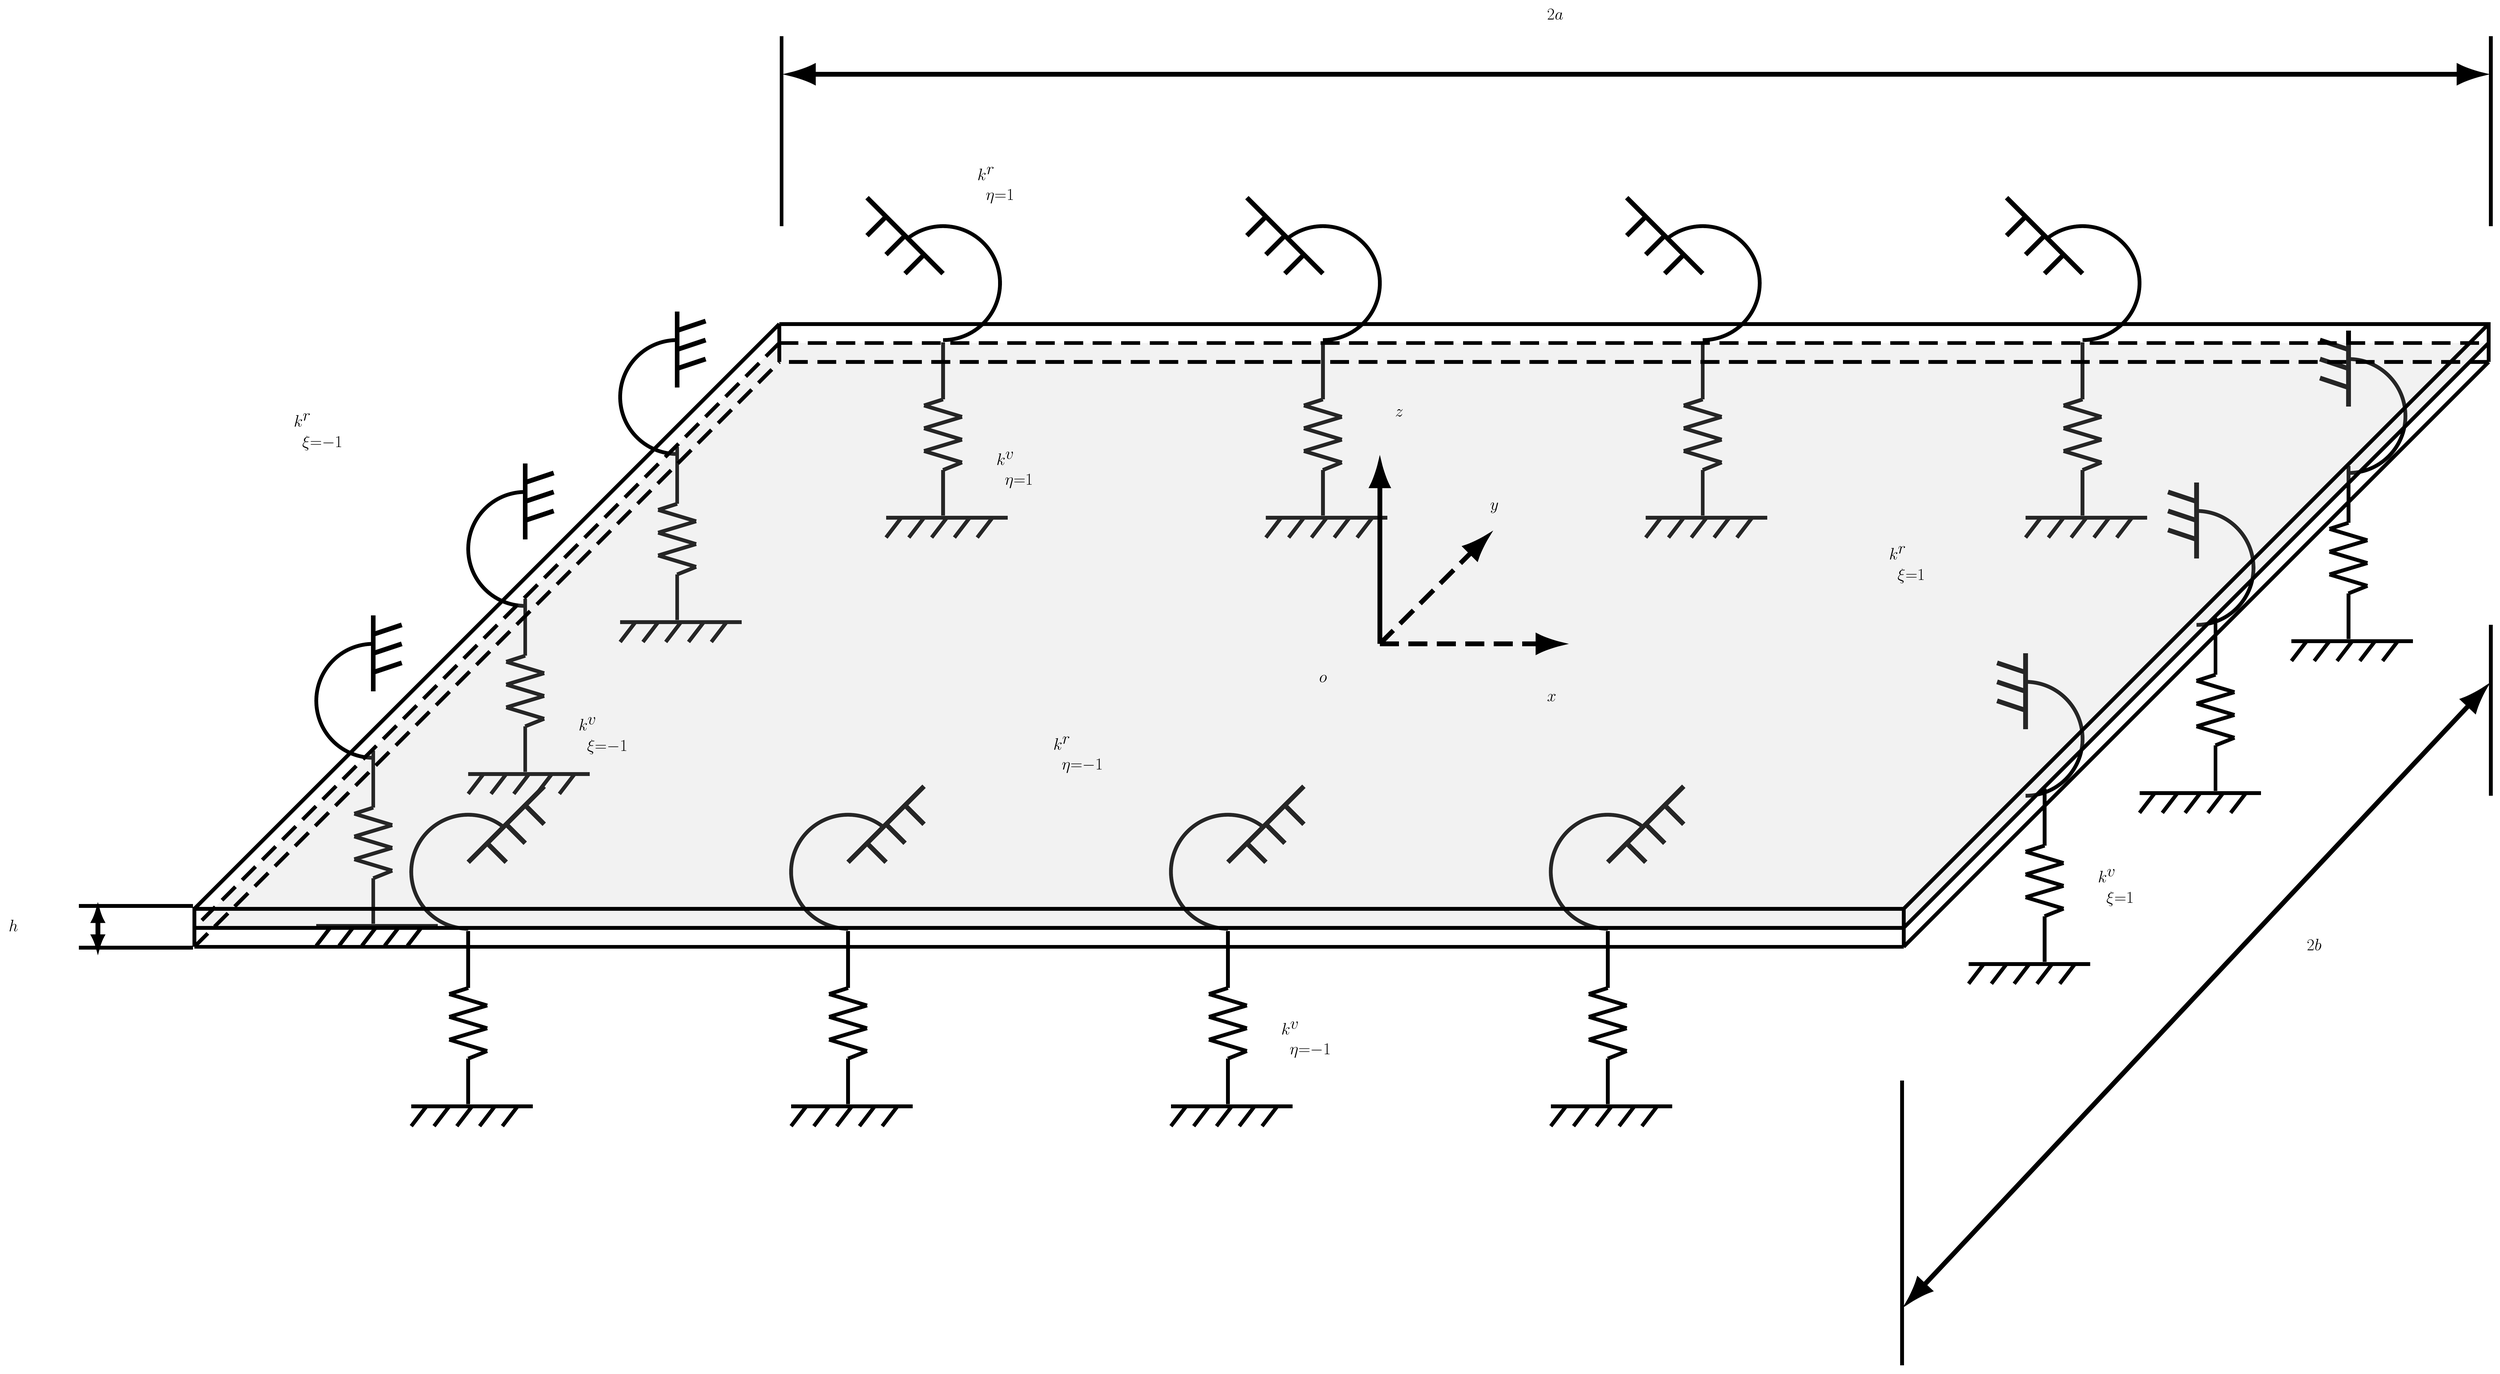
\begin{tikzpicture}[yscale=1]
	\tikzset{
	pics/boundary-box/.style={
		code={
			\begin{scope}[shift={(0mm,0mm)}]
				\definecolor{fc}{RGB}{204,204,204}
				\draw [fill=none, draw=black, line width=0.6mm] (000.0mm,0.0mm)
				-- ++(0.0mm,60.0mm)
				-- ++(-60.0mm,0.0mm)
				-- ++(0.0mm,-60.0mm)  % Adjusted the vertical length to 20mm
				-- ++(60.0mm,0.0mm)  % Adjusted the vertical length to 20mm
				-- cycle;
				\node [black, anchor=west, font=\fontsize{100}{0}\selectfont\bfseries] at (-40mm, 30mm) { $\textbf{?}$ };
			\end{scope}
		}
	}
}
\tikzset{
	pics/Mass-circle/.style={
		code={
			\draw[fill=gray!30, draw=black, line width=0.6mm] (0mm, 0mm) circle [radius=38mm];
		}
	}
}
\tikzset{
	pics/Beam/.style={
		code={\draw [fill=none,draw=black,line width=10.0mm] (000.0mm,0.mm)
			-- ++(600.0mm,0.0mm)
			;
			%% curvature
			\draw[fill=none, draw=gray, line width=4.0mm, dash pattern=on 20pt off 20pt] (000.0mm,0.mm) .. controls (200mm,-100mm) and (300mm,-50mm) .. (600.0mm,0mm);
			
			
		}
	}
}
\tikzset{
	pics/Spring-damp/.style={
		code={\begin{scope}[cm={0.4,0,0,0.4,(40.0mm,0mm)}]
				\draw [fill=none,draw=black,line width=2.0mm] (145.0mm,707.4mm)
				-- ++(0.0mm,33.0mm)
				;
				\draw [fill=none,draw=black,line width=2.0mm] (120.0mm,867.4mm)
				-- ++(50.0mm,-15.0mm)
				;
				\draw [fill=none,draw=black,line width=2.0mm] (170.0mm,852.4mm)
				-- ++(-50.0mm,-15.0mm)
				;
				\draw [fill=none,draw=black,line width=2.0mm] (120.0mm,837.4mm)
				-- ++(50.0mm,-15.0mm)
				;
				\draw [fill=none,draw=black,line width=2.0mm] (170.0mm,822.4mm)
				-- ++(-50.0mm,-15.0mm)
				;
				
				\draw [fill=none,draw=black,line width=2.0mm] (120.0mm,807.4mm)
				-- ++(50.0mm,-15.0mm)
				;
				
				\draw [fill=none,draw=black,line width=2.0mm] (170.0mm,792.4mm)
				-- (120.0mm,777.4mm)
				;
				
				\draw [fill=none,draw=black,line width=2.0mm] (120.0mm,777.4mm)
				-- ++(50.0mm,-15.0mm)
				;
				
				\draw [fill=none,draw=black,line width=2.0mm] (170.0mm,762.4mm)
				-- ++(-50.0mm,-15.0mm)
				;
				
				\draw [fill=none,draw=black,line width=2.0mm] (145.0mm,875.4mm)
				-- ++(-25.0mm,-8.0mm)
				;
				
				\draw [fill=none,draw=black,line width=2.0mm] (120.0mm,747.4mm)
				-- ++(25.0mm,-7.0mm)
				;
				
				\draw [fill=none,draw=black,line width=2.0mm] (145.0mm,875.4mm)
				-- (145.0mm,907.4mm)
				;
			\end{scope}
			% horizontal line above mass left
			\draw [fill=none,draw=black,line width=2.0mm] (58.0mm,363mm)
			-- ++(40.0mm,0.0mm)
			;
			
			%% damping left
			\begin{scope}[cm={0.4,0,0,-0.4,(0.0mm,645.9mm)}]
				\draw [fill=none,draw=black,line width=2.0mm] (115.0mm,827.7mm)
				-- ++(0.0mm,-35.3mm)
				-- (175.0mm,792.4mm)
				-- ++(0.0mm,35.0mm)
				;
				
				\draw [fill=none,draw=black,line width=2.0mm] (145.0mm,707.4mm)
				-- ++(0.0mm,85.0mm)
				;
				
				\draw [fill=none,draw=black,line width=2.0mm] (123.0mm,807.4mm)
				-- ++(44.0mm,0.0mm)
				;
				
				\draw [fill=none,draw=black,line width=2.0mm] (145.0mm,807.4mm)
				-- ++(0.0mm,100.0mm)
				;
			\end{scope}
			
			%% suspension arrow left
			\draw [fill=none,draw=black,line width=2.0mm] (58.0mm,283.4mm)
			-- ++(40.0mm,0.0mm)
			;
			\draw [fill=none,draw=black,line width=2.0mm] (78.0mm,363.4mm)
			-- ++(0mm,27.0mm)
			;
			%% vertical line upp
			\draw [fill=none,draw=black,line width=2.0mm] (78.0mm,283.4mm)
			-- ++(0.0mm,-30.0mm)
			;
		}
	}
}
\tikzset{
	pics/beam-Spring/.style={
		code={\begin{scope}[cm={0.4,0,0,0.4,(-38.0mm,-256.4mm)}]
				\draw [fill=none,draw=black,line width=2.0mm] (145.0mm,782.4mm)
				-- ++(0.0mm,-60.0mm)
				;
				\draw [fill=none,draw=black,line width=2.0mm] (120.0mm,867.4mm)
				-- ++(50.0mm,-15.0mm)
				;
				\draw [fill=none,draw=black,line width=2.0mm] (170.0mm,852.4mm)
				-- ++(-50.0mm,-15.0mm)
				;
				\draw [fill=none,draw=black,line width=2.0mm] (120.0mm,837.4mm)
				-- ++(50.0mm,-15.0mm)
				;
				\draw [fill=none,draw=black,line width=2.0mm] (170.0mm,822.4mm)
				-- ++(-50.0mm,-15.0mm)
				;
				\draw [fill=none,draw=black,line width=2.0mm] (120.0mm,807.4mm)
				-- ++(50.0mm,-15.0mm)
				;
				\draw [fill=none,draw=black,line width=2.0mm] (170.0mm,792.4mm)
				-- (145.0mm,782.4mm)
				;
				
				
			
				\draw [fill=none,draw=black,line width=2.0mm] (145.0mm,875.4mm)
				-- ++(-25.0mm,-8.0mm)
				;
				
				\draw [fill=none,draw=black,line width=2.0mm] (145.0mm,875.4mm)
				-- (145.0mm,950.4mm)
				;
			\end{scope}
			
		}
	}
}
\tikzset{
	pics/beam-arrow/.style={
		code={% bridge curve property 
			\draw [fill=none,draw=black,line width=2.0mm] (380.0mm,32.0mm)
			.. controls ++(85.0mm,-8.0mm) and ++(-60.0mm,-6.0mm) .. ++(135.0mm,-32.0mm)
			;
			%% arraw of bridge curve property 
			\draw [->, black, line width=6mm, >=stealth, shorten >=1pt] (515.0mm,0mm) -- ++(0.5,0); % Draws the arrowhead separately
			
		}
	}
}
\tikzset{
	pics/beam-prop-arrow/.style={
		code={% bridge curve deflection yx
			\draw [fill=none,draw=black,line width=2.0mm] (440.0mm,0.0mm)
			.. controls ++(85.0mm,5.0mm) and ++(-60.0mm,4.0mm) .. ++(135.0mm,36.0mm)
			;
			%% arraw of bridge curve deflection yx
			\draw [black, line width=2mm] (570.0mm,36.0mm) -- (580.0mm,36.0mm);
			\draw [->, black, line width=6mm, >=stealth, shorten >=1pt] (580.0mm,36.0mm) -- ++(0.5,0); % Draws the arrowhead separately
			
		}
	}
}
\tikzset{
	pics/mass-defle/.style={
		code={%% arraw of vehicle deflection yv 
			\draw [->,fill=none,draw=black,line width=2.50mm] (0.0mm,25.0mm)
			-- (30.0mm,25.0mm)
			-- (30.0mm,65.3mm)
			;			
		}
	}
}
\tikzset{
	pics/floor/.style={
		code={
			%  left
			\begin{scope}[cm={0.4,0,0,-0.4,(-42.0mm,377.0mm)}]
				\draw [fill=none,draw=black,line width=2.0mm] (30.0mm,939mm)
				-- (190.0mm,939mm)
				;
				\draw [fill=none,draw=black,line width=2.0mm] (50.0mm,939mm)
				-- (30.0mm,965mm)
				;
				\draw [fill=none,draw=black,line width=2.0mm] (80.0mm,939mm)
				-- (60.0mm,965mm)
				;
				\draw [fill=none,draw=black,line width=2.0mm] (110.0mm,939mm)
				-- (90.0mm,965mm)
				;
				\draw [fill=none,draw=black,line width=2.0mm] (140.0mm,939mm)
				-- (120.0mm,965mm)
				;
				\draw [fill=none,draw=black,line width=2.0mm] (170.0mm,939mm)
				-- (150.0mm,965mm)
				;
			\end{scope}
			
		}
	}
}
\tikzset{
	pics/beam-rotation/.style={
		code={
			%%% arc representing rotation or deflection
			\draw [-,fill=none,draw=black,line width=2.00mm] 
			(0.0mm,25.0mm) arc [start angle=270, end angle=90, radius=30mm];
			\draw [fill=none,draw=black,line width=2.5mm] (0.0mm,60mm)
			-- (0.0mm,100mm)
			;
			
			\draw [fill=none,draw=black,line width=2.5mm] (0.0mm,70mm)
			-- (15.0mm,75mm)
			;
			\draw [fill=none,draw=black,line width=2.5mm] (0.0mm,80mm)
			-- (15.0mm,85mm)
			;
			\draw [fill=none,draw=black,line width=2.5mm] (0.0mm,90mm)
			-- (15.0mm,95mm)
			;
			
		}
	}
}
\tikzset{
	pics/beam-rotation-bot/.style={
		code={
			%%% arc representing rotation or deflection
			\draw [-,fill=none,draw=black,line width=2.00mm] 
			(0.0mm,25.0mm) arc [start angle=270, end angle=50, radius=30mm];
			\draw [fill=none,draw=black,line width=2.5mm] (0.0mm,60mm)
			-- (40.0mm,100mm)
			;
			
			\draw [fill=none,draw=black,line width=2.5mm] (10mm,70mm)
			-- (20.0mm,60mm)
			;
			\draw [fill=none,draw=black,line width=2.5mm] (20mm,80mm)
			-- (30.0mm,70mm)
			;
			\draw [fill=none,draw=black,line width=2.5mm] (30mm,90mm)
			-- (40.0mm,80mm)
			;
			
		}
	}
}
\tikzset{
	pics/Rectangular-Plate/.style={
		code={
			% Define the vertices of the rectangular plate
			\coordinate (A) at (0, 1, 0);
			\coordinate (B) at (90, 1, 0);
			\coordinate (C) at (90, 2, 0);
			\coordinate (D) at (0, 2, 0);
			\coordinate (A') at (0, 1, 80);
			\coordinate (B') at (90, 1, 80);
			\coordinate (C') at (90, 2, 80);
			\coordinate (D') at (0, 2, 80);
			\coordinate (E) at (0, 0, 0);
			\coordinate (F) at (90, 0, 0);
			\coordinate (E') at (0, 0, 80);
			\coordinate (F') at (90, 0, 80);
			
			% Fill the surface AA'B'B with gray and transparent
			\fill[gray!50, fill opacity=0.2] (A) -- (A') -- (B') -- (B) -- cycle;
			
			% Draw the edges of the bottom face
			\draw[black, line width=2mm, dashed, dash pattern=on 10mm off 5mm] (A) -- (B); % AB dashed
			\draw[black, line width=2mm] (B) -- (C) -- (D); % Remaining edges solid
			\draw[black, line width=2mm, dashed, dash pattern=on 10mm off 5mm] (D) -- (A); % AD dashed
			\draw[black, line width=2mm, dashed, dash pattern=on 10mm off 5mm] (A) -- (E); % AB dashed
			\draw[black, line width=2mm, dashed, dash pattern=on 10mm off 5mm] (F) -- (E); % AB dashed
			\draw[black, line width=2mm, dashed, dash pattern=on 10mm off 5mm] (F) -- (B); % AB dashed
			\draw[black, line width=2mm, dashed, dash pattern=on 10mm off 5mm] (E') -- (E); % AB dashed

			% Draw the edges of the top face
			\draw[black, line width=2mm] (A') -- (B') -- (C') -- (D') -- cycle;
			
			% Draw the vertical edges connecting the bottom and top faces
			\draw[black, line width=2mm, dashed, dash pattern=on 10mm off 5mm] (A) -- (A'); % AA' dashed
			\draw[black, line width=2mm] (B) -- (B');
			\draw[black, line width=2mm] (C) -- (C');
			\draw[black, line width=2mm] (D) -- (D');
			\draw[black, line width=2mm] (F) -- (F');
			\draw[black, line width=2mm] (A') -- (E');
			\draw[black, line width=2mm] (B') -- (F');
			\draw[black, line width=2mm] (F') -- (E');
		}
	}
}



	%%%%%%%%%%%%%%%%%%%%%%%%%%%%%%%%% drawing
	%\pic at (700mm,0mm) {boundary-box};
	%\pic at (40mm,0mm) {boundary-box};
	\pic at (20mm,-25mm) {beam-rotation};
	\pic at (0mm,-120mm) {beam-Spring};
	\pic at (20mm,-90mm) {floor};
	\pic at (-60mm,-105mm) {beam-rotation};
	\pic at (-80mm,-200mm) {beam-Spring};
	\pic at (-60mm,-170mm) {floor};
	\pic at (-140mm,-185mm) {beam-rotation};
	\pic at (-160mm,-280mm) {beam-Spring};
	\pic at (-140mm,-250mm) {floor};

	%%%%%%%%%%%%
	\pic[xscale=-1] at (900mm,-35mm) {beam-rotation};
	\pic at (880mm,-130mm) {beam-Spring};
	\pic at (900mm,-100mm) {floor};
	\pic[xscale=-1] at (820mm,-115mm) {beam-rotation};
	\pic at (810mm,-210mm) {beam-Spring};
	\pic at (820mm,-180mm) {floor};
	\pic[xscale=-1] at (730mm,-205mm) {beam-rotation};
	\pic at (720mm,-300mm) {beam-Spring};
	\pic at (730mm,-270mm) {floor};
%%%%%%%%%%%%%%%%%%%%%%%%
	\pic[xscale=-1] at (160mm,35mm) {beam-rotation-bot};
	\pic at (140mm,-65mm) {beam-Spring};
	\pic at (160mm,-35mm) {floor};
	\pic[xscale=-1] at (360mm,35mm) {beam-rotation-bot};
	\pic at (340mm,-65mm) {beam-Spring};
	\pic at (360mm,-35mm) {floor};
	\pic[xscale=-1] at (560mm,35mm) {beam-rotation-bot};
	\pic at (540mm,-65mm) {beam-Spring};
	\pic at (560mm,-35mm) {floor};
	\pic[xscale=-1] at (760mm,35mm) {beam-rotation-bot};
	\pic at (740mm,-65mm) {beam-Spring};
	\pic at (760mm,-35mm) {floor};
	%%%%%%%%%
	\pic[xscale=1] at (510mm,-275mm) {beam-rotation-bot};
	\pic at (490mm,-375mm) {beam-Spring};
	\pic at (510mm,-345mm) {floor};
	\pic[xscale=1] at (310mm,-275mm) {beam-rotation-bot};
	\pic at (290mm,-375mm) {beam-Spring};
	\pic at (310mm,-345mm) {floor};
	\pic[xscale=1] at (110mm,-275mm) {beam-rotation-bot};
	\pic at (90mm,-375mm) {beam-Spring};
	\pic at (110mm,-345mm) {floor};
	\pic[xscale=1] at (-90mm,-275mm) {beam-rotation-bot};
	\pic at (-110mm,-375mm) {beam-Spring};
	\pic at (-90mm,-345mm) {floor};
	
	%%%%%%%%
    \pic at (3mm, 6, 3) {Rectangular-Plate};
    
    %%%%%%%%%%%%%%%%%%%%%
    %%% 2b
    \begin{scope}[shift={(-35mm,-180.0mm)}]
    	\draw[{Latex[length=18mm, width=12mm]}-{Latex[length=18mm, width=12mm]}, fill=none, draw=black, line width=2.5mm] 
    	(700mm,-270.0mm) -- (1010mm,60.0mm);
    	\draw [-,fill=none,draw=black,line width=2.mm] (700mm,-150.0mm)
    	-- (700mm,-300.0mm)
    	;
    	\draw [-,fill=none,draw=black,line width=2.mm] (1010mm,90.0mm)
    	-- (1010mm,000.0mm)
    	;
    \end{scope}
    %%% 2a
    \begin{scope}[shift={(-35mm,150.0mm)}]
    	\draw[{Latex[length=18mm, width=12mm]}-{Latex[length=18mm, width=12mm]}, fill=none, draw=black, line width=2.5mm] 
    	 (110mm,50.0mm)
    	-- (1010mm,50.0mm);
    	\draw [-,fill=none,draw=black,line width=2.mm] (110mm,70.0mm)
    	-- (110mm,-30.0mm)
    	;
    	\draw [-,fill=none,draw=black,line width=2.mm] (1010mm,70.0mm)
    	-- (1010mm,-30.0mm)
    	;
    \end{scope}
        %%% h
    \begin{scope}[shift={(-35mm,150.0mm)}]
    	\draw[{Latex[length=12mm, width=8mm]}-{Latex[length=12mm, width=8mm]}, fill=none, draw=black, line width=2.5mm] 
    	(-250mm,-385.0mm)
    	-- (-250mm,-415.0mm);
    	\draw [-,fill=none,draw=black,line width=2.mm] (-260mm,-388.0mm)
    	-- (-200mm,-388.0mm)
    	;
    	\draw [-,fill=none,draw=black,line width=2.mm] (-260mm,-410.0mm)
    	-- (-200mm,-410.0mm)
    	;
    \end{scope}
     %%% xyz
    \begin{scope}[shift={(30mm,-150.0mm)}]
    	\draw[-{Latex[length=18mm, width=12mm]}, fill=none, draw=black, line width=2.5mm, dashed, dash pattern=on 10mm off 5mm] 
    	(360mm,50.0mm) -- (460mm,50.0mm);
    	\draw[-{Latex[length=18mm, width=12mm]}, fill=none, draw=black, line width=2.5mm] 
    	(360mm, 50.0mm) -- (360mm, 150.0mm); 		
    	\draw[-{Latex[length=18mm, width=12mm]}, fill=none, draw=black, line width=2.5mm, dashed, dash pattern=on 10mm off 5mm] 
    	(360mm, 50.0mm) -- (420mm, 110.0mm);
    	
    	
    \end{scope}
	%%%%%%%%%%%%%%%% text
	
	\begin{scope}[shift={(16.9mm,-8.4mm)}]
		\node [black,anchor=west,font=\fontsize{140}{0}\selectfont] at (340mm,-110mm) { $o$ };
		\node [black,anchor=west,font=\fontsize{140}{0}\selectfont] at (460mm,-120mm) { $x$ };
		\node [black,anchor=west,font=\fontsize{140}{0}\selectfont] at (430mm,-20mm) { $y$ };
		\node [black,anchor=west,font=\fontsize{140}{0}\selectfont] at (380mm,30mm) { $z$ };
		\node [black,anchor=west,font=\fontsize{140}{0}\selectfont] at (460mm,240mm) { $2a$ };
		\node [black,anchor=west,font=\fontsize{140}{0}\selectfont] at (860mm,-250mm) { $2b$ };
		\node [black,anchor=west,font=\fontsize{140}{0}\selectfont] at (-350mm,-240mm) { $h$ };
		\node [black,anchor=west,font=\fontsize{140}{0}\selectfont] at (-50mm,-140mm) { $k^v_{\xi=-1}$ };
		\node [black,anchor=west,font=\fontsize{140}{0}\selectfont] at (-200mm,20mm) { $k^r_{\xi=-1}$ };
		\node [black,anchor=west,font=\fontsize{140}{0}\selectfont] at (750mm,-220mm) { $k^v_{\xi=1}$ };
	    \node [black,anchor=west,font=\fontsize{140}{0}\selectfont] at (640mm,-50mm) { $k^r_{\xi=1}$ };
	    \node [black,anchor=west,font=\fontsize{140}{0}\selectfont] at (320mm,-300mm) { $k^v_{\eta=-1}$ };
		\node [black,anchor=west,font=\fontsize{140}{0}\selectfont] at (200mm,-150mm) { $k^r_{\eta=-1}$ };
		\node [black,anchor=west,font=\fontsize{140}{0}\selectfont] at (170mm,0mm) { $k^v_{\eta=1}$ };
		\node [black,anchor=west,font=\fontsize{140}{0}\selectfont] at (160mm,150mm) { $k^r_{\eta=1}$ };
	\end{scope}
\end{tikzpicture}

	}
	\caption{\small The orthotropic rectangular plate with all edges elastically restrained.} 
	\label{fig:platemode}
\end{figure}
Consider a thin orthotropic rectangular plate of length $2a$ and width $2b$, with all four edges restrained by vertical translational springs $k^v$ and rotational springs $k^r$, as shown in \Cref{fig:platemode}. 
The coordinate origin is located at the center of the plate.

The governing differential equation for the free vibration of a thin orthotropic plate is given by \citep{xing2020improved}:  
%
\begin{equation}\label{eq:governing_EOM}
	D_{11}\frac{\partial^4w}{\partial \xi^4} + 2D_3\alpha^2\frac{\partial^4w}{\partial \xi^2 \partial \eta^2} + D_{22}\alpha^4\frac{\partial^4w}{\partial \eta^4} = \rho h\alpha^4\omega^2w,
\end{equation}
%
where $ \alpha = a / b $ is the aspect ratio; $ \xi = x / a $ and $ \eta = y / b $ are the normalized coordinates,
and the bending stiffness parameters are defined as:
%
\begin{equation}\label{eq:bd_stiff}
	\begin{split}
		&D_{11} = \frac{E_1h^3}{12(1-v_{12}v_{21})}, \qquad D_{22} = \frac{E_2h^3}{12(1-v_{12}v_{21})}, \\  
		&D_{66} = \frac{G_{12}h^3}{12}, \quad D_{12} = v_{12}D_{22} = v_{21}D_{11}, \quad D_3 = D_{12} + 2D_{66},
	\end{split}
\end{equation}
%
where $\rho$ and $h$ denote the mass density and thickness of the plate, respectively; $E_1$ and $E_2$ are the Young’s moduli in the $x$- and $y$-directions, respectively; $G_{12}$ is the shear modulus, and $v_{12}$ and $v_{21}$ are the Poisson’s ratios.

Instead of solving the free vibration of the thin orthotropic plate using \Cref{eq:governing_EOM}, it is suggested that the vibration of the thin plate can also be solved using the Rayleigh quotient variational principle \cite{xing2018overall}:
%
\begin{equation}\label{eq:Rayleigh}
	\begin{split}
		\delta U_{mag} &= \omega^2\,\delta T_0,
	\end{split}
\end{equation}
%
where $\delta$ denotes variation, $U_{mag}$ is the magnitude of the potential energy of the plate, and $\omega^2 T_0$ represents the magnitude of the kinetic energy of the plate.
The potential energy of the plate can be expressed as \cite{xing2020extended}:
%
\begin{equation}\label{eq:poten_energy}
	\begin{split}
		U^{I} &= \frac{1}{2}\iint \Big[D_{11}\left(\frac{\partial^2 W}{\partial x^2}\right)^2 + 2D_{12}\frac{\partial^2 W}{\partial x^2}\frac{\partial^2 W}{\partial y^2} + D_{22}\left(\frac{\partial^2 W}{\partial y^2}\right)^2 \\
		&\qquad + 4D_{66}\left(\frac{\partial^2 W}{\partial x \partial y}\right)^2\Big] \, \mathrm{d}x \, \mathrm{d}y.
	\end{split}
\end{equation}
%
And the kinetic energy is:
%
\begin{equation}\label{eq:kine_energy}
	\begin{split}
		T &= \frac{1}{2}\iint \rho h \left(\frac{\partial W}{\partial t}\right)^2 \, \mathrm{d}x \, \mathrm{d}y.
	\end{split}
\end{equation}

Assuming the solution of the deflection $ W(x, y; t) = w(x, y) e^{i \omega t} $ for harmonic plate motion, 
where $ \ii = \sqrt{-1} $, $ w(x, y) $ is the mode shape, and $ \omega $ is the radial frequency.  
By substituting $ W(x, y; t) = w(x, y) e^{i \omega t} $ into \Cref{eq:poten_energy,eq:kine_energy} and expressing the system in dimensionless coordinates, we have:
%
\begin{equation}\label{eq:poten_energy_mag}
	\begin{split}
		U_{\text{mag}}^{I} &= \frac{ab}{2} \iint \left[ \frac{D_{11}}{a^4} \left( \frac{\partial^2 w}{\partial \xi^2} \right)^2 + \frac{2 D_{12}}{a^2 b^2} \frac{\partial^2 w}{\partial \xi^2} \frac{\partial^2 w}{\partial \eta^2} + \frac{D_{22}}{b^4} \left( \frac{\partial^2 w}{\partial \eta^2} \right)^2 \right. \\
		&\quad \left. + \frac{4 D_{66}}{a^2 b^2} \left( \frac{\partial^2 w}{\partial \xi \partial \eta} \right)^2 \right] \, \mathrm{d} \xi \, \mathrm{d} \eta,
	\end{split}
\end{equation}
%
and
%
\begin{equation}\label{eq:kine_energy_mag}
	\begin{split}
		T &= \omega^2 \frac{ab}{2} \rho h \iint w^2 \, \mathrm{d} \xi \, \mathrm{d} \eta = \omega^2 T_0
	\end{split},
\end{equation}
%
The separable form of the mode shape function $ w(\xi, \eta)$ is given by:
%
\begin{equation}\label{eq:displace_func}
	w(\xi, \eta) = \phi(\xi) \psi(\eta),
\end{equation}
%
where $ \phi(\xi) $ and $\psi(\eta) $ can be expressed as:
\begin{subequations}\label{eq:phi_psi_solution}
	\begin{align}
		\phi(\xi) &= A_1 \sin{(\alpha_1 \xi)} + A_2 \cos{(\alpha_1 \xi)} + A_3 \sinh{(\beta_1 \xi)} + A_4 \cosh{(\beta_1 \xi)},\label{eq:phi_solution1}\\
		\psi(\eta) &= B_1 \sin{(\alpha_2 \eta)} + B_2 \cos{(\alpha_2 \eta)} + B_3 \sinh{(\beta_2 \eta)} + B_4 \cosh{(\beta_2 \eta)}. \label{eq:phi_solution2}
	\end{align}
\end{subequations}

Based on \Cref{eq:Rayleigh}, the frequencies $\omega_x$ and $\omega_y$, corresponding to the mode shapes $\phi(\xi)$ and $\psi(\eta)$, respectively, are assumed to be independent of each other.

\subsection{Dynamic stiffness matrix corresponding to $\omega_x$}\label{sec:DSMx}
For given general homogeneous boundary conditions, we can first assume that the mode shape $\psi(\eta)$ corresponding to the $y$-direction is known. 
Supposing the edges of the plate in both the $x$- and $y$-directions are elastically restrained by homogeneous vertical translational and rotational springs.
The vertical translational and rotational springs at the $\xi = -1$ end are defined as $k^v_{\xi = -1}$ and $k^r_{\xi = -1}$, respectively, and at the $\xi = 1$ end as $k^v_{\xi = 1}$ and $k^r_{\xi = 1}$, respectively. 
Thus, the potential energy along the supported edge in the $x$-direction can be expressed by:
%
\begin{equation}\label{eq:poten_energy_edgex}
	\begin{split}
		U^{II} &=  \int\left[k^r_{\xi=-1} \left( \frac{\partial W}{\partial x} \right)^2 + k^v_{\xi=-1} \left( W \right)^2\right]_{x=-a} \id y\\
		&\qquad +  \int\left[k^r_{\xi=1} \left( \frac{\partial W}{\partial x} \right)^2 + k^v_{\xi=1} \left( W \right)^2\right]_{x=a} \id y.
	\end{split}
\end{equation}
%
From \Cref{eq:poten_energy_edgex}, the magnitude of total potential energy along the edges in the $x$-direction is obtained as:
%
\begin{equation}\label{eq:poten_energy_edgex2}
	\begin{split}
		U^{II}_{mag} &= ab \int\left[\frac{k^r_{\xi=-1}}{a^3} \left( \frac{\partial w}{\partial \xi} \right)^2 + \frac{k^v_{\xi=-1}}{a} \left( w \right)^2\right]_{\xi=-1} \, \id \eta \\
		&\qquad + ab \int\left[\frac{k^r_{\xi=1}}{a^3} \left( \frac{\partial w}{\partial \xi} \right)^2 + \frac{k^v_{\xi=1}}{a} \left( w \right)^2\right]_{\xi=1} \, \id \eta.
	\end{split}
\end{equation}
%
The magnitude of potential energy of the plate in the $x$-direction can be obtained from \Cref{eq:poten_energy_mag,eq:poten_energy_edgex2} as:
%
\begin{equation}\label{eq:poten_energy_tolx}
	\begin{split}
		U_{mag} &= U^{I}_{mag} + U^{II}_{mag} \\
		&= \frac{ab}{2} \iint \left[ \frac{D_{11}}{a^4} \left( \frac{\partial^2 w}{\partial \xi^2} \right)^2 + \frac{2 D_{12}}{a^2 b^2} \frac{\partial^2 w}{\partial \xi^2} \frac{\partial^2 w}{\partial \eta^2} + \frac{D_{22}}{b^4} \left( \frac{\partial^2 w}{\partial \eta^2} \right)^2 \right. \\
		&\qquad \left.  + \frac{4 D_{66}}{a^2 b^2} \left( \frac{\partial^2 w}{\partial \xi \partial \eta} \right)^2 \right] \, \id\xi \, \id\eta + ab \int \left[\frac{k^r_{\xi=1}}{a^3} \left( \frac{\partial w}{\partial \xi} \right)^2 + \frac{k^v_{\xi=1}}{a} \left( w \right)^2 \right]_{\xi=1} \, \id \eta \\
		&\qquad  + ab \int \left[\frac{k^r_{\xi=-1}}{a^3} \left( \frac{\partial w}{\partial \xi} \right)^2 + \frac{k^v_{\xi=-1}}{a} \left( w \right)^2 \right]_{\xi=-1} \, \id \eta
	\end{split}
\end{equation}
%
By substituting \Cref{eq:displace_func} into \Cref{eq:poten_energy_tolx}, we have:
%
\begin{equation}\label{eq:poten_energy_tolx2}
	\begin{split}
		U_{mag}&=U^{I}_{mag}+U^{II}_{mag}\\
		&=\frac{ab}{2} \int_{-1}^{1} \left[ \frac{D_{11}}{a^4}I_1 \left( \frac{\id^2\phi }{\id \xi^2} \right)^2 + \frac{2 D_{12}}{a^2 b^2}I_2 \frac{\id^2\phi }{\id \xi^2}\phi  + \frac{D_{22}}{b^4}I_4  \phi^2 \right. \\
		&\qquad \left. + \frac{4 D_{66}}{a^2 b^2}I_3 \left( \frac{\id \phi }{\id \xi}\right)^2 \right] \, \id\xi +abI_1 \left[\frac{k^r_{\xi=-1}}{a^3} \left( \frac{\id \phi}{\id \xi} \right)^2+ \frac{k^v_{\xi=-1}}{a} \left( \phi \right)^2\right]_{\xi=-1}\\
		&\qquad+abI_1 \left[\frac{k^r_{\xi=1}}{a^3} \left( \frac{\id \phi}{\id \xi} \right)^2+ \frac{k^v_{\xi=1}}{a} \left( \phi \right)^2\right]_{\xi=1},
	\end{split}
\end{equation}
%
where the integral parameters are defined as:
%
\begin{equation}\label{eq:inte_phi_text}  
	\begin{split}  
		&I_1 = \int_{-1}^{1} \psi^2 \, \id\eta, \\  
		&I_2 = \int_{-1}^{1} \left( \frac{\id^2 \psi}{\id \eta^2} \psi \right) \, \id\eta, \\  
		&I_3 = \int_{-1}^{1} \left( \frac{\id \psi}{\id \eta} \right)^2 \, \id\eta, \\  
		&I_4 = \int_{-1}^{1} \left( \frac{\id^2 \psi}{\id \eta^2} \right)^2 \, \id\eta.  
	\end{split}  
\end{equation}   
%
By taking \Cref{eq:displace_func} into account, the coefficient $T_0$ of the kinetic energy from \Cref{eq:kine_energy_mag} for the plate can be expressed as:
%
\begin{equation}\label{eq:kine_energyx}
	\begin{split}
		T_0 = \frac{ab}{2}\rho h\iint w^2 \, \id \xi \, \id \eta = \frac{ab}{2}\rho h I_1\int_{-1}^{1} \phi^2 \, \id \xi.
	\end{split}
\end{equation}
%
Take the Rayleigh principle in the form:
%
\begin{equation}\label{eq:Rayleighx}
	\begin{split}
		\delta U_{mag} &= \omega_x^2 \, \delta T_0.
	\end{split}
\end{equation}
%
By substituting \Cref{eq:poten_energy_tolx2,eq:kine_energyx} into \Cref{eq:Rayleighx}, and relieving $\delta \phi$ and $\delta\frac{\id  \phi}{\id \xi}$ in \Cref{eq:Rayleighx} by variation calculus, yields:
%
\begin{equation}\label{eq:Rayleighx2}
	\begin{split}
		0 &= \int_{-1}^{1} \bigg[ \frac{D_{11}}{a^4} I_1 \frac{\id^4 \phi}{\id \xi^4} 
		+ \bigg( \frac{2D_{12}}{a^2b^2} I_2 - \frac{4D_{66}}{a^2b^2} I_3 \bigg) \frac{\id^2 \phi}{\id \xi^2} \\
		&\qquad + \bigg( \frac{D_{22}}{b^4} I_4 - \omega_x^2 \rho h I_1 \bigg) \phi \bigg] \delta \phi \, \id \xi \\
		&\qquad + \frac{2k^v_{\xi=-1}}{a} I_1 \big(\phi \delta \phi\big)_{\xi=-1} 
		+ \frac{2k^v_{\xi=1}}{a} I_1 \big(\phi \delta \phi\big)_{\xi=1} \\
		&\qquad + \bigg[ \bigg( \frac{4D_{66}}{a^2b^2} I_3 - \frac{D_{12}}{a^2b^2} I_2 \bigg) \frac{\id \phi}{\id \xi} 
		- \frac{D_{11}}{a^4} I_1 \frac{\id^3 \phi}{\id \xi^3} \bigg] \delta \phi \Big|^{\xi=1}_{\xi=-1} \\
		&\qquad + \bigg( \frac{D_{12}}{a^2b^2} I_2 \phi + \frac{D_{11}}{a^4} I_1 \frac{\id^2 \phi}{\id \xi^2} \bigg) 
		\delta\frac{\id  \phi}{\id \xi} \Big|^{\xi=1}_{\xi=-1} \\
		&\qquad + \frac{2k^r_{\xi=-1}}{a^3} I_1 \bigg(\frac{\id \phi}{\id \xi}\delta \frac{\id \phi}{\id \xi}\bigg)_{\xi=-1} 
		+ \frac{2k^r_{\xi=1}}{a^3} I_1 \bigg(\frac{\id \phi}{\id \xi} \delta\frac{\id \phi}{\id \xi}\bigg)_{\xi=1}.
	\end{split}
\end{equation}
%
Thus, the governing differential equation in the $ x $-direction can be obtained from the integration part in \Cref{eq:Rayleighx2}:
%
\begin{equation}\label{eq:ODEx}
		\frac{\id^4 \phi}{\id \xi^4}+ 2\alpha^2\left(\frac{D_{12}I_2}{D_{11}I_1}-2\frac{D_{66}I_3}{D_{11}I_1}\right)\frac{\id^2 \phi}{\id \xi^2}+\left(\alpha^4\frac{D_{22}I_4}{D_{11}I_1}-a^4\Omega_x^4\right)\phi=0,
\end{equation}
%
where $\Omega_x = \sqrt[4]{\omega_x^2 \rho h / D_{11}}$.
By substituting $\phi(\xi) = A e^{\mu \xi}$ into \Cref{eq:ODEx}, yields:
%
\begin{equation}\label{eq:ODEx2}
	\begin{split}
		\mu^4 + 2\alpha^2\left(\frac{D_{12}I_2}{D_{11}I_1}-2\frac{D_{66}I_3}{D_{11}I_1}\right)\mu^2 + \left(\alpha^4\frac{D_{22}I_4}{D_{11}I_1}-a^4\Omega_x^4\right) = 0.
	\end{split}
\end{equation}
%
The solution for $\mu$ can be expressed as:
%
\begin{equation}\label{eq:mu}
	\begin{split}
		\mu_{1,2} = \pm\textit{i} \alpha_1, \qquad \mu_{3,4} = \pm \beta_1,
	\end{split}
\end{equation}
%
where,
%
\begin{subequations}\label{eq:alphax}
	\begin{align}
		\alpha_1 &= \alpha \sqrt{\sqrt{\left(\frac{D_{12}I_2}{D_{11}I_1}-2\frac{D_{66}I_3}{D_{11}I_1}\right)^2 - \frac{D_{22}I_4}{D_{11}I_1} + b^4\Omega_x^4} + \frac{D_{12}I_2}{D_{11}I_1} - 2\frac{D_{66}I_3}{D_{11}I_1}},\label{eq:alphax1}\\
		\beta_1 &= \alpha \sqrt{\sqrt{\left(\frac{D_{12}I_2}{D_{11}I_1}-2\frac{D_{66}I_3}{D_{11}I_1}\right)^2 - \frac{D_{22}I_4}{D_{11}I_1} + b^4\Omega_x^4} - \frac{D_{12}I_2}{D_{11}I_1} + 2\frac{D_{66}I_3}{D_{11}I_1}}.\label{eq:alphax2}
	\end{align}
\end{subequations}
%
The boundary conditions along the edges in the $x$-direction can be obtained from the remaining $\delta \phi$ and $\delta \frac{\id \phi}{\id \xi}$ parts in \Cref{eq:Rayleighx2}. 
The shear force equilibrium can be obtained from the $\delta \phi$ part:
%
\begin{equation}\label{eq:inertial_forcex}
	\begin{split}
		&\left[ \left( \frac{4D_{66}}{a^2b^2} I_3 - \frac{D_{12}}{a^2b^2} I_2 \right) \frac{\id \phi}{\id \xi} 
		- \frac{D_{11}}{a^4} I_1 \frac{\id^3 \phi}{\id \xi^3} \right] \Big|^{\xi=1}_{\xi=-1}\\
		&\qquad+ \frac{2k^v_{\xi=-1}}{a} I_1 \left(\phi\right)_{\xi=-1}
		 + \frac{2k^v_{\xi=1}}{a} I_1 \left(\phi\right)_{\xi=1} = 0,
	\end{split}
\end{equation}
%
and from the $\delta \frac{\id \phi}{\id \xi}$ part, the bending moment equilibrium:
%
\begin{equation}\label{eq:inertial_forcex2}
	\begin{split}	
		\left( \frac{D_{12}}{a^2b^2} I_2 \phi + \frac{D_{11}}{a^4} I_1 \frac{\partial^2 \phi}{\partial \xi^2} \right) 
		\Big|^{\xi=1}_{\xi=-1} 
		&+ \frac{2k^r_{\xi=-1}}{a^3} I_1 \left(\frac{\partial \phi}{\partial \xi}\right)_{\xi=-1} \\
		& \qquad\frac{2k^r_{\xi=1}}{a^3} I_1 \left(\frac{\partial \phi}{\partial \xi}\right)_{\xi=1} = 0.
	\end{split}
\end{equation}
%
Thus, we can obtain the shear force and bending moment equilibrium along the edges $\xi = -1$ and $\xi = 1$ from \Cref{eq:inertial_forcex,eq:inertial_forcex2}, respectively, as:
%
\begin{subequations}\label{eq:boundaryx}
	\begin{align}
		&  \frac{\id^3 \phi}{\id \xi^3} - \alpha^2\left( \frac{4D_{66}I_3}{D_{11}I_1}  - \frac{D_{12}I_2}{D_{11}I_1}  \right) \frac{\id \phi}{\id \xi} 
		+\frac{2a^3k^v_{\xi=-1}}{D_{11}}\phi = 0, \quad &\xi = -1, \\
		& \frac{\id^2 \phi}{\id \xi^2} + \frac{\alpha^2 D_{12} I_2}{D_{11} I_1} \phi - \frac{2a k^r_{\xi=-1}}{D_{11}} \frac{\id \phi}{\id \xi} = 0, \quad &\xi = -1, \\
		& \frac{\id^3 \phi}{\id \xi^3} - \alpha^2\left( \frac{4D_{66}I_3}{D_{11}I_1}  - \frac{D_{12}I_2}{D_{11}I_1}  \right) \frac{\id \phi}{\id \xi} 
		-\frac{2a^3 k^v_{\xi=1}}{D_{11}} \phi = 0, \quad &\xi = 1, \\
		& \frac{\id^2 \phi}{\id \xi^2} + \frac{\alpha^2 D_{12} I_2}{D_{11} I_1} \phi + \frac{2a k^r_{\xi=1}}{D_{11}} \frac{\id \phi}{\id \xi} = 0, \quad &\xi = 1.
	\end{align}
\end{subequations}
%
Substituting \Cref{eq:phi_solution1} into \Cref{eq:boundaryx}, and denoting $ k^{v*}_{\xi} = \frac{2a^3 k^v_{\xi}}{D_{11}} $, $ k^{r*}_{\xi} = \frac{2a k^r_{\xi}}{D_{11}} $, $ S_{\alpha_1}=\sin\alpha_1 $, $ C_{\alpha_1}=\cos\alpha_1 $, $ Sh_{\alpha_1}=\sinh\alpha_1 $, $ Ch_{\alpha_1}=\cosh\alpha_1 $, $S_{\beta_1}= \sin\beta_1 $, $C_{\beta_1}=\cos\beta_1$, $Sh_{\beta_1}=\sinh\beta_1 $, and $  Ch_{\beta_1}=\cosh\beta_1 $, we have:
%
\begin{equation}\label{eq:ABx}
	\begin{split}
		&\left[ \begin{array}{c}
			\gamma_1 C_{\alpha_1} - k^{v*}_{\xi=-1} S_{\alpha_1} \\ 
			\gamma_3 S_{\alpha_1} + k^{r*}_{\xi=-1} \alpha_1 C_{\alpha_1} \\ 
			-\gamma_1 C_{\alpha_1} + k^{v*}_{\xi=1} S_{\alpha_1} \\ 
			\gamma_3 S_{\alpha_1} + k^{r*}_{\xi=1} \alpha_1 C_{\alpha_1}
		\end{array} 
		\begin{array}{c}
			\gamma_1 S_{\alpha_1} + k^{v*}_{\xi=-1} C_{\alpha_1} \\ 
			-\gamma_3 C_{\alpha_1} + k^{r*}_{\xi=-1} \alpha_1 S_{\alpha_1} \\ 
			\gamma_1 S_{\alpha_1} + k^{v*}_{\xi=1} C_{\alpha_1} \\ 
			\gamma_3 C_{\alpha_1} - k^{r*}_{\xi=1} \alpha_1 S_{\alpha_1}
		\end{array} 
		\begin{array}{c}
			\gamma_2 Ch_{\beta_1} - k^{v*}_{\xi=-1} Sh_{\beta_1} \\ 
			\gamma_4 Sh_{\beta_1} + k^{r*}_{\xi=-1} \beta_1 Ch_{\beta_1} \\ 
			-\gamma_2 Ch_{\beta_1} + k^{v*}_{\xi=1} Sh_{\beta_1} \\ 
			\gamma_4 Sh_{\beta_1} + k^{r*}_{\xi=1} \beta_1 Ch_{\beta_1}
		\end{array} \right. \\ 
		&\quad
		\left. \begin{array}{c}
			-\gamma_2 Sh_{\beta_1} + k^{v*}_{\xi=-1} Ch_{\beta_1} \\ 
			-\gamma_4 Ch_{\beta_1} - k^{r*}_{\xi=-1} \beta_1 Sh_{\beta_1} \\ 
			-\gamma_2 Sh_{\beta_1} + k^{v*}_{\xi=1} Ch_{\beta_1} \\ 
			\gamma_4 Ch_{\beta_1} + k^{r*}_{\xi=1} \beta_1 Sh_{\beta_1}
		\end{array} \right] \begin{Bmatrix}
			A_1 \\ A_2 \\ A_3 \\ A_4
		\end{Bmatrix} =  \begin{Bmatrix}
			0 \\ 0 \\ 0 \\ 0
		\end{Bmatrix},
	\end{split}
\end{equation}
%
or,
%
\begin{equation}\label{eq:ABx1}
		\mathbf{R}_x \mathbf{A} = \mathbf{0},
\end{equation}
%
where,
%
\begin{equation}\label{eq:gamma}
	\begin{split}
		&\gamma_1 = -\alpha_1^3 - \alpha^2 \left( \frac{4D_{66}S_3}{D_{11}I_1} - \frac{D_{12}I_2}{D_{11}I_1} \right) \alpha_1, \\
		&\gamma_2 = \beta_1^3 - \alpha^2 \left( \frac{4D_{66}S_3}{D_{11}I_1} - \frac{D_{12}I_2}{D_{11}I_1} \right) \beta_1, \\
		&\gamma_3 = -\alpha_1^2 + \frac{\alpha^2 D_{12} I_2}{D_{11} I_1}, \\
		&\gamma_4 = \beta_1^2 + \frac{\alpha^2 D_{12} I_2}{D_{11} I_1}.
	\end{split}
\end{equation}
%
Note that the classic boundary conditions can be obtained by selecting extremely large or small spring stiffness constants.
For non-trivial solutions, the characteristic equation or eigenvalue equation is obtained from the determinant of the matrix $\mathbf{R}_x$ in \Cref{eq:ABx1}, which must be zero.
However, solving these transcendental equations are cunmbersome and tedious, thus the DSM is introducted to avoid the ineffective computation.

To develop its dynamic stiffness matrix, with the help of \Cref{eq:phi_solution1}, the vertical displacement and rotation corresponding to the mode shape $\phi(\xi)$ along the $x$-direction at edges $\xi = -1$ and $\xi = 1$ can be expressed as:
%
\begin{equation}\label{eq:UBx}
	\begin{split}
		\begin{Bmatrix}
			\phi_{\xi=-1}\\\frac{\id \phi}{\id \xi}_{\xi=-1}\\\phi_{\xi=1}\\\frac{\id \phi}{\id \xi}_{\xi=1}
		\end{Bmatrix}
		= \begin{bmatrix}
			-S_{\alpha_1}&C_{\alpha_1}&-Sh_{\beta_1}&Ch_{\beta_1}\\
			\alpha_1 C_{\alpha_1}/a&\alpha_1S_{\alpha_1}/a&\beta_1Ch_{\beta_1}/a&-\beta_1Sh_{\beta_1}/a\\
			S_{\alpha_1}&C_{\alpha_1}&Sh_{\beta_1}&Ch_{\beta_1}\\
			\alpha_1 C_{\alpha_1}/a&-\alpha_1S_{\alpha_1}/a&\beta_1Ch_{\beta_1}/a&\beta_1Sh_{\beta_1}/a
		\end{bmatrix}
		\begin{Bmatrix}
			A_1\\A_2\\A_3\\A_4
		\end{Bmatrix} ,
	\end{split}
\end{equation}
%
or,
%
\begin{equation}\label{eq:UBx1}
	\mathbf{\delta}_x= \mathbf{Q}_x\mathbf{A}.
\end{equation}
%
Note that the eigenvector $\mathbf{A}$ can be expressed by multiplying the inverse matrix $\mathbf{Q}_x^{-1}$ on the left side of \Cref{eq:UBx1}, and then substituting $\mathbf{A}$ into \Cref{eq:ABx1}, we obtain:
%
\begin{equation}\label{eq:DSM_eqx}
	\mathbf{R}_x \mathbf{A}=\mathbf{R}_x\mathbf{Q}_x^{-1}\mathbf{\delta}_x = \mathbf{0}.
\end{equation}
%
where the dynamic stiffness matrix, denoted as $\mathbf{K}_x = \mathbf{R}_x\mathbf{Q}_x^{-1}$, can be obtained from \Cref{eq:DSM_eqx}. 
This matrix can be used to compute the natural frequencies of the system instead of solving the eigenvalue equation, 
and the method for the computation will be given in \Cref{sec:WWA}.

\subsection{Dynamic stiffness matrix corresponding to $\omega_y$}\label{sec:DSMy}
In this section, the mode shape $\phi(\xi)$ derived in $\Cref{sec:DSMx}$ is utilized to obtain the dynamic stiffness matrix in the $y$-direction.  
The vertical translational and rotational springs at $\eta = -1$ are denoted as $k^v_{\eta = -1}$ and $k^r_{\eta = -1}$, respectively, while those at $\eta = 1$ are represented by $k^v_{\eta = 1}$ and $k^r_{\eta = 1}$.

The magnitude of total potential energy along the edges in the $y$-direction is given by:  
%
\begin{equation}\label{eq:poten_energy_edgey2}  
	\begin{split}  
		U^{III}_{mag} &= ab \int \left[ \frac{k^r_{\eta=-1}}{a^3} \left( \frac{\partial w}{\partial \eta} \right)^2 + \frac{k^v_{\eta=-1}}{a} w^2 \right]_{\eta=-1} \id \xi \\  
		&\qquad + ab \int \left[ \frac{k^r_{\eta=1}}{a^3} \left( \frac{\partial w}{\partial \eta} \right)^2 + \frac{k^v_{\eta=1}}{a} w^2 \right]_{\eta=1} \id \xi.  
	\end{split}  
\end{equation} 
% 
The magnitude of potential energy of the plate in the $y$-direction can be obtained from
\Cref{eq:poten_energy_mag,eq:poten_energy_edgey2} as:
%
\begin{equation}\label{eq:poten_energy_toly}
	\begin{split}
		U_{mag}&=U^{I}_{mag}+U^{III}_{mag}\\
		&=\frac{ab}{2} \iint \left[ \frac{D_{11}}{a^4} \left( \frac{\partial^2 w}{\partial \xi^2} \right)^2 + \frac{2 D_{12}}{a^2 b^2} \frac{\partial^2 w}{\partial \xi^2} \frac{\partial^2 w}{\partial \eta^2} + \frac{D_{22}}{b^4} \left( \frac{\partial^2 w}{\partial \eta^2} \right)^2 \right. \\
		&\qquad \left.  + \frac{4 D_{66}}{a^2 b^2}\left( \frac{\partial^2 w}{\partial \xi \partial \eta} \right)^2 \right] \, \id\xi \, \id\eta+ab \int \left[ \frac{k^r_{\eta=1}}{b^3} \left( \frac{\partial w}{\partial \eta} \right)^2 + \frac{k^v_{\eta=1}}{b} \left( w \right)^2 \right]_{\eta=1} \id\xi\\
		&\qquad+ab \int \left[ \frac{k^r_{\eta=-1}}{b^3} \left( \frac{\partial w}{\partial \eta} \right)^2 + \frac{k^v_{\eta=-1}}{b} \left( w \right)^2 \right]_{\eta=-1} \id\xi.
	\end{split}
\end{equation}
%
By substituting \Cref{eq:displace_func} into \Cref{eq:poten_energy_toly}, we obtain:  
%
\begin{equation}\label{eq:poten_energy_toly2}
	\begin{split}
		U_{mag} &= U^{I}_{mag} + U^{III}_{mag} \\
		&= \frac{ab}{2} \int_{-1}^{1} \left[ \frac{D_{11}}{a^4} J_4 \psi^2 
		+ \frac{2D_{12}}{a^2b^2} J_2 \frac{\id^2\psi }{\id \eta^2} \psi 
		+ \frac{D_{22}}{b^4} J_1 \left(\frac{\id^2\psi }{\id \eta^2} \right)^2 \right. \\
		&\qquad \left. + \frac{4D_{66}}{a^2b^2} J_3 \left(\frac{\id \psi }{\id \eta} \right)^2 \right] \, \id\eta  + abJ_1 \left[ \frac{k^r_{\eta=1}}{b^3} \left( \frac{\id \psi}{\id \eta} \right)^2
		+ \frac{k^v_{\eta=1}}{b}  \left(\psi\right)^2 \right]_{\eta=1} \\
		&\qquad + abJ_1 \left[ \frac{k^r_{\eta=-1}}{b^3} \left( \frac{\id \psi}{\id \eta} \right)^2
		+ \frac{k^v_{\eta=-1}}{b} \left(\psi\right)^2 \right]_{\eta=-1},
	\end{split}
\end{equation}
%
where the integral parameters are defined as:  
%
\begin{equation}\label{eq:inte_psi}  
	\begin{split}  
		&J_1 = \int_{-1}^{1} \phi^2 \, \id\xi, \\  
		&J_2 = \int_{-1}^{1} \left( \frac{\id^2\phi}{\id\xi^2} \phi \right) \, \id\xi, \\  
		&J_3 = \int_{-1}^{1} \left( \frac{\id\phi}{\id\xi} \right)^2 \, \id\xi, \\  
		&J_4 = \int_{-1}^{1} \left( \frac{\id^2\phi}{\id\xi^2} \right)^2 \, \id\xi.  
	\end{split}  
\end{equation}  
%
The coefficient $T_0$ of the kinetic energy from \Cref{eq:kine_energy_mag} for the plate can be expressed as:
%
\begin{equation}\label{eq:kine_energyy}
	\begin{split}
		T_0 &= \frac{ab}{2} \rho h J_1 \int_{-1}^{1} \psi^2 \, \id\eta.
	\end{split}
\end{equation}
%
Take the Rayleigh principle in the form:
%
\begin{equation}\label{eq:Rayleighy}
	\begin{split}
		\delta U_{mag} &= \omega_y^2 \, \delta T_0.
	\end{split}
\end{equation}
%
By substituting \Cref{eq:poten_energy_toly2,eq:kine_energyy} into \Cref{eq:Rayleighy}, and relieving $ \delta \psi $ and $\delta\frac{\id \psi}{\id \eta}$ in \Cref{eq:Rayleighy} by variation calculus, yields:
%
\begin{equation}\label{eq:Rayleighy2}
	\begin{split}
		0 &= \int_{-1}^{1} \left[ \frac{D_{22}}{b^4} J_1 \frac{d^4 \psi}{\id \eta^4} 
		+ \left( \frac{2D_{12}}{a^2b^2} J_2 - \frac{4D_{66}}{a^2b^2} J_3 \right) \frac{\id^2 \psi}{\id \eta^2} \right. \\
		&\qquad \left. + \left( \frac{D_{11}}{a^4} J_4 - \omega_y^2 \rho h J_1 \right) \psi \right] \delta \psi \, \id\eta \\
		&\qquad + \frac{2k^v_{\eta=-1}}{b} J_1 (\psi \delta \psi)_{\eta=-1} 
		+ \frac{2k^v_{\eta=1}}{b} J_1 (\psi \delta \psi)_{\eta=1} \\
		&\qquad + \left[ \left( \frac{4D_{66}}{a^2b^2} J_3 - \frac{D_{12}}{a^2b^2} J_2 \right) \frac{\id \psi}{\id \eta} 
		- \frac{D_{22}}{b^4} J_1 \frac{\id^3 \psi}{\id \eta^3} \right] \delta \psi \Big|^{\eta=1}_{\eta=-1} \\
		&\qquad + \left( \frac{D_{12}}{a^2b^2} J_2 \psi + \frac{D_{22}}{b^4} J_1 \frac{\id^2 \psi}{\id \eta^2} \right) 
		\delta\frac{\id  \psi}{\id \eta} \Big|^{\eta=1}_{\eta=-1} \\
		&\qquad + \frac{2k^r_{\eta=-1}}{b^3} J_1 \left( \frac{\id \psi}{\id \eta} \delta\frac{\id \psi}{\id \eta} \right)_{\eta=-1} 
		+ \frac{2k^r_{\eta=1}}{b^3} J_1 \left( \frac{\id \psi}{\id \eta} \delta\frac{\id \psi}{\id \eta} \right)_{\eta=1}.
	\end{split}
\end{equation}
%
Thus, the governing differential equation in the $y$-direction can be obtained from the integration part in \Cref{eq:Rayleighy2}:
%
\begin{equation}\label{eq:ODEy}
		\frac{\id^4 \psi}{\id \eta^4} + \frac{2}{\alpha^2}\left(\frac{D_{12}J_2}{D_{22}J_1} - 2\frac{D_{66}J_3}{D_{22}J_1}\right)\frac{\id^2 \psi}{\id \eta^2} + \left( \frac{D_{11}J_4}{\alpha^4D_{22}J_1} - \frac{b^4D_{11}}{D_{22}} \Omega_y^4 \right) \psi = 0,
\end{equation}
%
where $\Omega_y = \sqrt[4]{{\omega_y^2 \rho h}/D_{11}}$.
By substituting $\psi(\eta) = B e^{\lambda \eta}$ into \Cref{eq:ODEy}, yields:
%
\begin{equation}\label{eq:ODEy2}
	\begin{split}
		\lambda^4 + \frac{2}{\alpha^2} \left( \frac{D_{12}J_2}{D_{22}J_1} - 2\frac{D_{66}J_3}{D_{22}J_1} \right) \lambda^2 + \left( \frac{D_{11}J_4}{\alpha^4D_{22}J_1} - \frac{b^4D_{11}}{D_{22}} \Omega_y^4 \right) = 0.
	\end{split}
\end{equation}
%
The solution for $\lambda$ can be expressed as:
%
\begin{equation}\label{eq:lambda}
	\begin{split}
		\lambda_{1,2} &= \pm \textit{i} \alpha_2, \qquad \lambda_{3,4} = \pm \beta_2,
	\end{split}
\end{equation}
%
where,
%
\begin{subequations}\label{eq:beta}
	\begin{align}
		\alpha_2 &= \frac{1}{\alpha} \sqrt{ \sqrt{ \left( \frac{D_{12}J_2}{D_{22}J_1} - 2\frac{D_{66}J_3}{D_{22}J_1} \right)^2 - \frac{D_{11}J_4}{D_{22}J_1} + \frac{a^4 D_{11}}{D_{22}} \Omega_y^4 } + \frac{D_{12}J_2}{D_{22}J_1} - 2 \frac{D_{66}J_3}{D_{22}J_1}}, \\
		\beta_2 &= \frac{1}{\alpha} \sqrt{ \sqrt{ \left( \frac{D_{12}J_2}{D_{22}J_1} - 2 \frac{D_{66}J_3}{D_{22}J_1} \right)^2 - \frac{D_{11}J_4}{D_{22}J_1} + \frac{a^4 D_{11}}{D_{22}} \Omega_y^4 } - \frac{D_{12}J_2}{D_{22}J_1} + 2 \frac{D_{66}J_3}{D_{22}J_1}}.
	\end{align}
\end{subequations}
%
The boundary conditions along the edges in the $y$-direction can be obtained from the remaining $\delta \psi$ and $\delta \frac{\id \psi}{\id \eta}$ parts in \Cref{eq:Rayleighy2}. 
The shear force equilibrium can be obtained from the $\delta \psi$ part:
%
\begin{equation}\label{eq:inertial_forcey}
	\begin{split}
		& \left[ \left( \frac{4D_{66}}{a^2b^2} J_3 - \frac{D_{12}}{a^2b^2} J_2 \right) \frac{\id \psi}{\id \eta} 
		- \frac{D_{22}}{b^4} J_1 \frac{\id^3 \psi}{\id \eta^3} \right] \Big|^{\eta=1}_{\eta=-1} \\
		&\qquad + \frac{2k^v_{\eta=-1}}{b} J_1 (\psi )_{\eta=-1} + \frac{2k^v_{\eta=1}}{b} J_1 (\psi )_{\eta=1} = 0,
	\end{split}
\end{equation}
%
and from the $\delta \frac{\id \psi}{\id \eta}$ part, the bending moment equilibrium:
%
\begin{equation}\label{eq:inertial_forcey2}	
 \begin{split}
 	\left( \frac{D_{12}}{a^2b^2} J_2 \psi + \frac{D_{22}}{b^4} J_1 \frac{\id^2 \psi}{\id \eta^2} \right) 
 	\Big|^{\eta=1}_{\eta=-1} 
 	&+ \frac{2k^r_{\eta=-1}}{b^3} J_1 \left( \frac{\id \psi}{\id \eta} \right)_{\eta=-1} \\
 	&\qquad+ \frac{2k^r_{\eta=1}}{b^3} J_1 \left( \frac{\id \psi}{\id \eta} \right)_{\eta=1}=0.
 \end{split}
\end{equation}
%
Thus, we can obtain the shear force and bending moment equilibrium along the edges $\eta = -1$ and $\eta = 1$ from \Cref{eq:inertial_forcey,eq:inertial_forcey2}, respectively, as:
%
\begin{subequations}\label{eq:boundaryy}
	\begin{align}
		&  \frac{\id^3 \psi}{\id \eta^3}-\left( \frac{4D_{66}J_3}{\alpha^2D_{22}J_1}  - \frac{D_{12}J_2}{\alpha^2D_{22}J_1}  \right) \frac{\id \psi}{\id \eta} 
		+\frac{2b^3k^v_{\eta=-1}}{D_{22}}\psi=0,\quad &\eta=-1,\\
		& \frac{\id^2 \psi}{\id \eta^2}+\frac{D_{12}J_2}{\alpha^2D_{22}J_1} \psi -\frac{2bk^r_{\eta=-1}}{D_{22}}\frac{\id\psi }{\id \eta}=0,\quad &\eta=-1,\\
		&  \frac{\id^3 \psi}{\id \eta^3}-\left( \frac{4D_{66}J_3}{\alpha^2D_{22}J_1}  - \frac{D_{12}J_2}{\alpha^2D_{22}J_1}  \right) \frac{\id \psi}{\id \eta} 
		-\frac{2b^3k^v_{\eta=1}}{D_{22}}\psi=0,\quad &\eta=1,\\
		&\frac{\id^2 \psi}{\id \eta^2}+\frac{D_{12}J_2}{\alpha^2D_{22}J_1} \psi +\frac{2bk^r_{\eta=1}}{D_{22}}\frac{\id\psi }{\id \eta}=0,\quad &\eta=1.
	\end{align}
\end{subequations}
%
Substituting \Cref{eq:phi_solution2} into \Cref{eq:boundaryy} and denoting
$k^{v*}_{\eta} = \frac{2b^3 k^v_{\eta}}{D_{22}} $, 
$ k^{r*}_{\eta} = \frac{2b k^r_{\eta}}{D_{22}} $, 
$S_{\alpha_2}=\sin\alpha_2  $, 
$ C_{\alpha_2}=\cos\alpha_2  $, 
$ Sh_{\alpha_2}=\sinh\alpha_2  $, 
$ Ch_{\alpha_2}=\cosh\alpha_2 $, 
$ S_{\beta_2}=\sin\beta_2 $, 
$ C_{\beta_2}=\cos\beta_2 $, 
$ Sh_{\beta_2}=\sinh\beta_2$, and 
$Ch_{\beta_2}= \cosh\beta_2$, 
We obtain:
%
\begin{equation}\label{eq:ABy}
	\begin{split}
		&\left[ \begin{array}{c}
			\zeta_1C_{\alpha_2}-k^{v*}_{\eta=-1}S_{\alpha_2} \\ \zeta_3S_{\alpha_2}+k^{r*}_{\eta=-1}\alpha_2C_{\alpha_2} \\ -\zeta_1C_{\alpha_2}+k^{v*}_{\eta=1}S_{\alpha_2} \\ \zeta_3S_{\alpha_2}+k^{r*}_{\eta=1}\alpha_2C_{\alpha_2}
		\end{array} \begin{array}{c}
			\zeta_1S_{\alpha_2}+k^{v*}_{\eta=-1}C_{\alpha_2} \\ -\zeta_3C_{\alpha_2}+k^{r*}_{\eta=-1}\alpha_2S_{\alpha_2} \\ \zeta_1S_{\alpha_2}+k^{v*}_{\eta=1}C_{\alpha_2} \\ \zeta_3C_{\alpha_2}-k^{r*}_{\eta=1}\alpha_2S_{\alpha_2}
		\end{array} \begin{array}{c}
			\zeta_2Ch_{\beta_2}-k^{v*}_{\eta=-1}Sh_{\beta_2} \\ \zeta_4Sh_{\beta_2}+k^{r*}_{\eta=-1}\beta_2Ch_{\beta_2} \\ -\zeta_2Ch_{\beta_2}+k^{v*}_{\eta=1}Sh_{\beta_2} \\ \zeta_4Sh_{\beta_2}+k^{r*}_{\eta=1}\beta_2Ch_{\beta_2}
		\end{array} \right. \\
		&\quad
		\left. \begin{array}{c}
			-\zeta_2Sh_{\beta_2}+k^{v*}_{\eta=-1}Ch_{\beta_2} \\ -\zeta_4Ch_{\beta_2}-k^{r*}_{\eta=-1}\beta_2Sh_{\beta_2} \\ -\zeta_2Sh_{\beta_2}+k^{v*}_{\eta=1}Ch_{\beta_2} \\ \zeta_4Ch_{\beta_2}+k^{r*}_{\eta=1}\beta_2Sh_{\beta_2}
		\end{array} \right]\begin{Bmatrix}
			B_1\\B_2\\B_3\\B_4
		\end{Bmatrix}=\begin{Bmatrix}
			0\\0\\0\\0
		\end{Bmatrix},
	\end{split}
\end{equation}
%
or,
%
\begin{equation}\label{eq:ABy1}
	\mathbf{R}_y \mathbf{B} = \mathbf{0},
\end{equation}
%
where,
%
\begin{equation}\label{eq:gammay}
	\begin{split}
		&\zeta_1=-\alpha_2^3-\left( \frac{4D_{66}J_3}{\alpha^2D_{22}J_1}  - \frac{D_{12}J_2}{\alpha^2D_{22}J_1}  \right)\alpha_2,\\
		&\zeta_2=\beta_2^3-\left( \frac{4D_{66}T_3}{\alpha^2D_{22}J_1}  - \frac{D_{12}J_2}{\alpha^2D_{22}J_1}  \right)\beta_2,\\
		&\zeta_3=-\alpha_2^2+\frac{D_{12}J_2}{\alpha^2D_{22}J_1},\\
		&\zeta_4=\beta_2^2+\frac{D_{12}J_2}{\alpha^2D_{22}J_1}.
	\end{split}
\end{equation}
%
With the help of \Cref{eq:phi_solution2}, the vertical displacement and rotation corresponding to the mode shape $\psi$ along the $y$-direction at the edges $\eta = -1$ and $\eta = 1$ can be expressed as:
%
\begin{equation}\label{eq:UBy}
	\begin{split}
		\begin{Bmatrix}
			\psi_{\eta=-1}\\\frac{\id \psi}{\id \eta}_{\eta=-1}\\\psi_{\eta=1}\\\frac{\id \psi}{\id \eta}_{\eta=1}
		\end{Bmatrix}
		= \begin{bmatrix}
			-S_{\alpha_2} & C_{\alpha_2} & -Sh_{\beta_2} & Ch_{\beta_2} \\
			\frac{\alpha_2 C_{\alpha_2}}{b} & \frac{\alpha_2 S_{\alpha_2}}{b} & \frac{\beta_2 Ch_{\beta_2}}{b} & -\frac{\beta_2 Sh_{\beta_2}}{b} \\
			S_{\alpha_2} & C_{\alpha_2} & Sh_{\beta_2} & Ch_{\beta_2} \\
			\frac{\alpha_2 C_{\alpha_2}}{b} & -\frac{\alpha_2 S_{\alpha_2}}{b} & \frac{\beta_2 Ch_{\beta_2}}{b} & \frac{\beta_2 Sh_{\beta_2}}{b}
		\end{bmatrix}
		\begin{Bmatrix}
			B_1\\B_2\\B_3\\B_4
		\end{Bmatrix},		
	\end{split}
\end{equation}
%
or,
%
\begin{equation}\label{eq:UBy1}
	\mathbf{\delta}_y= \mathbf{Q}_y\mathbf{B}.
\end{equation}
%
Note that the eigenvector $\mathbf{B}$ can be expressed by multiplying the inverse matrix $\mathbf{Q}_y^{-1}$ on the left-hand side of \Cref{eq:UBy1}, and then substituting $\mathbf{B}$ into \Cref{eq:ABy1}, we obtain:
%
\begin{equation}\label{eq:DSM_eqy}
	\mathbf{R}_y\mathbf{B}=\mathbf{R}_y \mathbf{Q}_x^{-1} 
	\mathbf{\delta}_y = \mathbf{0},
\end{equation}
%
where the dynamic stiffness matrix, denoted as $\mathbf{K}_y = \mathbf{R}_y \mathbf{Q}_y^{-1}$, can be obtained from \Cref{eq:DSM_eqy}.

\section{Frequency and mode shape computation}\label{sec:WWA}
\subsection{Wittrick–Williams algorithm and enhancement}\label{sec:WWA2}
The Wittrick–Williams (W-W) algorithm \cite{wittrick1971general} is an effective method for determining the natural frequencies from the dynamic stiffness matrix with high reliability. 
Instead of directly solving the equations, the algorithm computes the total number $J$ of natural frequencies below a given frequency $\omega^*$, which is represented as:
\begin{equation}\label{eq:WWalgorithm}
	J(\omega^*) = J_0(\omega^*) + s\{\mathbf{K}^{\Delta}(\omega^*)\} = J_0(\omega^*) + J_k(\omega^*),
\end{equation}
where $J_0$ represents the number of natural frequencies of the structure with all ends fully clamped, $\mathbf{K}^{\Delta}$ is the upper triangular matrix obtained from the dynamic stiffness matrix $\mathbf{K}$ after applying Gaussian elimination, and $J_k(\omega^*)$ denotes the number of negative elements in the leading diagonal of $\mathbf{K}^{\Delta}$.

It should be noted that the $J_0$ count is a crucial aspect when applying the W-W algorithm. Many previous studies use a sufficiently fine mesh or enough terms in series expansions to capture all fully clamped natural frequencies, ensuring computational accuracy \cite{banerjee2015dynamic}. However, this approach can make the application process cumbersome. 
To address this issue, the fully clamped problem can be replaced with a simply supported problem, where the Navier solution for the simply supported plate is used to count $J_0$ \citep{liu2015exact}. 
Nevertheless, since analytical solutions in DSM methods involve an infinite series of Fourier terms, a sufficient number of truncation terms is required to ensure accuracy and convergence.   


In fact, $ J_0 $ can be indirectly determined by evaluating the number of natural frequencies $ J $ of the structure under specific boundary conditions, which are generally different from the original boundary conditions \cite{han2018improved}:
%
\begin{equation}\label{eq:J_o_pin}
	J_0(p_1,\omega^*) = J(\bar{p}_1,\omega^*) - J_k(\bar{p}_1,\omega^*),
\end{equation}
%
where $ p_1 $ denotes the fully clamped supports, and $ \bar{p}_1 $ denotes specific supports, which are typically simply supported, guided, or a combination of the two.
For these specific boundary conditions, the eigenvalue equations of SOV type solution take the form of a single harmonic function.
By substituting \Cref{eq:J_o_pin} into \Cref{eq:WWalgorithm} we get the algorithm as:  
%
\begin{equation}\label{eq:new_WWalgorithm}
	J(p,\omega^*) = J(\bar{p}_1,\omega^*) - J_k(\bar{p}_1,\omega^*) + J_k(p,\omega^*)
\end{equation} 
%
where $p$ represents the original boundary conditions of the structure.
Therefore, the challenge of determining $J_0(p_1, \omega^*)$ can be transformed into the problem of solving $ J(\bar{p}_1, \omega^*)$ instead. 
By considering fully simply supported boundary conditions, the eigenvalue equation corresponding to the natural frequency parameter $ \Omega_x $ can be obtained from the determinant of the coefficient matrix $ \mathbf{R}_x $ in \Cref{eq:ABx}, as given by:
%
\begin{equation}\label{eq:SSx} 
	\sin 2\alpha_1 = 0.
\end{equation}
%
With the help of \Cref{eq:alphax1,eq:SSx}, the closed-form solution of the $n_x$-th simply supported frequency $\Omega_{x,n_x}$ for the given $n_y$-order $\psi_{n_y}(\eta)$ can be expressed as:
%
\begin{equation}\label{eq:J_simpx}
	\Omega_{x,n_x} =
	\frac{1}{b} \sqrt[4]{%
		%\large % slightly smaller than \Large
		\begin{aligned}
			&\left[\left(\frac{n_x\pi}{2\alpha}\right)^2 - \frac{D_{12}S_2}{D_{11}S_1} + 2 \frac{D_{66}S_3}{D_{11}S_1}\right]^2 - \left(\frac{D_{12}S_2}{D_{11}S_1} - 2 \frac{D_{66}S_3}{D_{11}S_1}\right)^2 \\
			&+ \frac{D_{22}S_4}{D_{11}S_1}.
		\end{aligned}
	}
\end{equation}
%
For $\Omega_{x,n_x} \leq \Omega_x^* < \Omega_{x,n_{x+1}}$, $J(\bar{p}_1, \Omega_x^*) = n_x$.
Similarly, the closed-form solution of the $n_y$-th simply supported frequency $\Omega_{y,n_y}$ for the given $n_x$-order $\phi_{n_x}(\xi)$ can be expressed as:
%
\begin{equation}\label{eq:J_simpy}
	\Omega_{y,n_y}= 
	\frac{1}{a} \sqrt[4]{%
		\begin{aligned}
			&\frac{D_{22}}{D_{11}}\left\{\left[\left(\frac{n_y\pi\alpha}{2}\right)^2 - \frac{D_{12}T_2}{D_{22}T_1} + 2 \frac{D_{66}T_3}{D_{22}T_1}\right]^2 - \left(\frac{D_{12}T_2}{D_{22}T_1} - 2 \frac{D_{66}T_3}{D_{22}T_1}\right)^2\right. \\
			&\left.  + \frac{D_{11}T_4}{D_{22}T_1}\right\}.
		\end{aligned}
	}
\end{equation}
%
For $\Omega_{y,n_y} \leq \Omega_y^* < \Omega_{y,n_{y+1}}$, $J(\bar{p}_1, \Omega_y^*) = n_y$.
According to the relationships 
$\Omega_x = \sqrt[4]{{\omega_x^2 \rho h}/{D_{11}}}$ and\ $\Omega_y = \sqrt[4]{{\omega_y^2 \rho h}/{D_{11}}}$, 
the values of $J(\bar{p}_1, \omega_x^*)$ and $J(\bar{p}_1, \omega_y^*)$ can be derived from $J(\bar{p}_1, \Omega_x^*)$ and $J(\bar{p}_1, \Omega_y^*)$, respectively. Therefore, this refined W-W algorithm can be applied to estimate the lower and upper bounds of the frequency range, denoted as $\omega_l$ and $\omega_u$, yielding an approximation for the frequency $\omega_a \in (\omega_l, \omega_u)$.
\subsection{Mode shape computation}
The mode shape coefficients $ A_1 $ to $ A_4 $ and $ B_1 $ to $ B_4$ in the eigenvectors $\mathbf{A}$ and $\mathbf{B}$ for all classic boundary conditions are provided in \cite{xing2020extended}. 
Alternatively, these coefficients can also be obtained through a simple numerical method, which this work presents as an approach.
Here, we illustrate solving the eigenvector $\mathbf{A}$ as an example.
By assuming the exact natural frequency as $\omega_k$, we can expand the coefficient matrix $ \mathbf{R}_{x} $ in \Cref{eq:ABx} using a first-order Taylor series about $\omega_a$:
%
\begin{equation}\label{eq:Taylor}
	\mathbf{R}_{x,k}(\omega_k)\mathbf{A}_k = \mathbf{R}_{x,a}\mathbf{A}_k + (\omega_k - \omega_a)\mathbf{R}'_{x,a}\mathbf{A}_k + O\left((\omega_k - \omega_a)^2\right) = 0.
\end{equation}
%
Ignoring higher-order terms, an eigenvalue problem can be derived from \Cref{eq:Taylor}:
%
\begin{equation}\label{eq:Newgeigen}
	(\mathbf{R}^{'}_{x,a})^{-1} \mathbf{R}_{x,a} \mathbf{A} = (\omega_a - \omega_k)\mathbf{A} = \tau \mathbf{A}.
\end{equation}
%
This eigenvalue problem can be solved using the inverse iteration procedure \cite{yuan2004second}:
%
\begin{equation}\label{eq:Inversepower}
	\bar{\mathbf{A}}^{(i+1)} = \mathbf{R}_{x,a}^{-1} \mathbf{R}^{'}_{x,a} \mathbf{A}^{(i)},	
\end{equation}
%
where the initial guess for $\mathbf{A}^{(0)}$ is a column vector consisting of four randomly generated elements, each of which falls within the range (0,1). The updated eigenvalue for the next step can be obtained as:
%
\begin{equation}\label{eq:Newgeigenvalue}
	\tau^{(i+1)} = \frac{1}{\bar{A}_j^{(i+1)}},
\end{equation}
%
where,
%
\begin{equation}\label{eq:updatetau}
	\mid \bar{A}_j^{(i+1)} \mid = \max(\mid \bar{A}_1^{(i+1)} \mid, \mid \bar{A}_2^{(i+1)} \mid, \mid\bar{A}_3^{(i+1)}\mid , \mid \bar{A}_4^{(i+1)} \mid).
\end{equation}
%
The updated eigenvector can be obtained as:
%
\begin{equation}\label{eq:updateeigenvalue}
	\mathbf{A}^{(i+1)} = \tau^{(i+1)} \bar{\mathbf{A}}^{(i+1)}.
\end{equation}
%
The procedure can be controlled by the error tolerance \( \epsilon \) or maximum allowed steps \( i_{\text{max}} \):
%
\begin{subequations}
	\begin{align}
		\max \mid A_n^{(i+1)} - A_n^{(i)} \mid < \epsilon, \\ 
		i = i_{\text{max}}.
	\end{align}
\end{subequations}
%
Note that the mode shape coefficients $A_1$ to $A_4$ obtained from $\mathbf{A}^{(i+1)}$ are applied for the elastically restrained boundary conditions.

\subsection{Application procedure}\label{sec:Application procedure}
The procedure of the proposed method is as follows:   
\begin{itemize}[]
	\item \textbf{Step 1} Assume initial integral parameters $I^{(0)}_1, I^{(0)}_2, I^{(0)}_3$, and $I^{(0)}_4$ in the $y$-direction. Using the given boundary conditions at $\xi = -1$ and $\xi = 1$, determine $\mathbf{K}^{(0)}_x$ from \Cref{eq:DSM_eqx}. 
	Then, apply the computational algorithms in \Cref{sec:WWA2} to compute the lower and upper bounds of the $n_x$-th non-dimensional frequency parameter, $2a\Omega^{(0)}_{l,x,n_x}$ and $2a\Omega^{(0)}_{u,x,n_x}$, and take the average $2a\Omega^{(0)}_{x,n_x} = (2a\Omega^{(0)}_{l,x,n_x} + 2a\Omega^{(0)}_{u,x,n_x})/2$ along with its corresponding mode shape $\phi^{(0)}_{n_x}$, where $n_x = 1, 2, 3, \ldots$.
	
	\item \textbf{Step 2} Use $\phi^{(0)}_{n_x}$ as the prescribed mode to determine $\mathbf{K}^{(1)}_y$ in \Cref{eq:DSM_eqy}, considering the boundary conditions at $\eta = -1$ and $\eta = 1$. 
	Apply the computational algorithms to obtain the $n_y$-th frequency parameter $2a\Omega^{(1)}_{y,n_y}$ and its corresponding mode shape $\psi^{(1)}_{n_y}$, where $n_y = 1, 2, 3, \ldots$. This completes the first iteration cycle.  
	
	\item \textbf{Step 3} Use $\psi^{(1)}_{n_y}$ as the prescribed $n_y$-th mode shape in the $y$-direction to compute $\mathbf{K}^{(1)}_x$ from \Cref{eq:DSM_eqx}, then determine the $n_x$-th frequency parameter $2a\Omega^{(1)}_{x,n_x}$ and its corresponding mode shape $\phi^{(1)}_{n_x}$.  
	
	\item \textbf{Step 4} Use $\phi^{(1)}_{n_x}$ as the prescribed mode in the $x$-direction to compute the $n_y$-th frequency parameter $2a\Omega^{(2)}_{y,n_y}$ and its corresponding mode shape $\psi^{(2)}_{n_y}$, completing the second iteration cycle.  
	
	\item \textbf{Step 5} Stop the iteration if $\lvert 2a\Omega^{(i)}_{x,n_x} - 2a\Omega^{(i+1)}_{x,n_x} \rvert \leq \Delta 2a\Omega$ or $\lvert 2a\Omega^{(i)}_{y,n_y} - 2a\Omega^{(i+1)}_{y,n_y} \rvert \leq \Delta 2a\Omega$, where $\Delta 2a\Omega = 2a\Omega_u - 2a\Omega_l$. Here, $2a\Omega_l$ and $2a\Omega_u$ are the lower and upper bounds of the frequency parameter range, within which the actual frequency parameter $2a\Omega$ lies, i.e., $2a\Omega \in (2a\Omega_l, 2a\Omega_u)$. The quantity $\Delta 2a\Omega$ represents the frequency parameter interval used in the W-W algorithm.
	
	\item \textbf{Step 6} Finally, construct the $(n_x, n_y)$-th mode shape as $w(\xi, \eta) = \phi_{n_x}(\xi) \psi_{n_y}(\eta)$ using \Cref{eq:displace_func}.  
\end{itemize}



\FloatBarrier
\section{Numerical Results}  
This section presents the numerical validation of the proposed method for classic boundary conditions and rotationally restrained boundary conditions.  
For all numerical calculations, the initial integral parameters are assumed as $I^{(0)}_1=1$, $I^{(0)}_2=1$, $I^{(0)}_3=1$, and $I^{(0)}_4=10$ in the $y$-direction, serving as the starting point of \textbf{Step 1} for any mode in all boundary conditions.  
In this section, the interval between the upper and lower bounds of the non-dimensional frequency parameter, $2a\Delta\Omega$, is set to 0.005, limiting the error range.  
According to our numerical calculations, two iteration cycles are generally sufficient to meet the convergence requirement (i.e., $\lvert 2a\Omega^{(i)}_{x} - 2a\Omega^{(i+1)}_{x} \rvert \leq \Delta 2a\Omega$ or $\lvert 2a\Omega^{(i)}_{y} - 2a\Omega^{(i+1)}_{y} \rvert \leq \Delta 2a\Omega$) for most cases, with at most three cycles required when applying the iterative procedure in \Cref{sec:Application procedure}.
 
 

\subsection{Classical boundary conditions}
In this subsection, the proposed method is validated by comparison with the extended SOV method \cite{xing2020extended}.  
The properties of the orthotropic plate, consistent with those in \cite{xing2020extended}, are as follows:  
$E_1 = 185 \nugpa$, $E_2 = 10.5 \nugpa$, $G_{12} = 7.3 \nugpa$, $\rho = 1600 \urho$, and $\nu_{12} = 0.28$.
  
The translational springs ($k^v_\xi$) and rotational springs ($k^r_\xi$) along all edges can be set to zero or infinity (represented as $1 \times 10^{15} \ustif$ in the numerical calculations of this study) to obtain different classic boundary conditions.  

The results for SSSS, SCSF, GCGC, CCCC, SSCC, SCCC, GGCC, CCFF, CFCF, CFFF, and FFFF boundary conditions are presented in \Cref{tab:sov1,tab:sov2,tab:sov3}. 
These results demonstrate high accuracy compared to the extended SOV method, with difference remaining smaller than the frequency parameter interval $2a\Delta\Omega=0.005$. 
The frequency parameters in both directions are equal ($2a\Omega_x - 2a\Omega_y = 0$) in almost all cases, with a few exceptions where $2a\Omega_x - 2a\Omega_y = 0.005$. 
In fact, higher accuracy compared to the extended SOV method can be achieved if the frequency parameter interval $2a\Delta\Omega$ is set smaller than 0.005. It should be noted that the accuracy improves only by reducing $2a\Delta\Omega$, and no additional iterations are required according to our calculations.
\Cref{fig:FFFF} shows the first six nonzero mode shapes of a square orthotropic plate with FFFF boundary conditions, where the mode shape coefficients are calculated using the numerical method developed in this study. 
Instead of selecting fixed expressions for the mode shape coefficients based on specific boundary conditions, our method is applicable to all boundary conditions.


\begin{figure}
	\centering
	\begin{subfigure}[b]{0.49\textwidth}
		\centering
		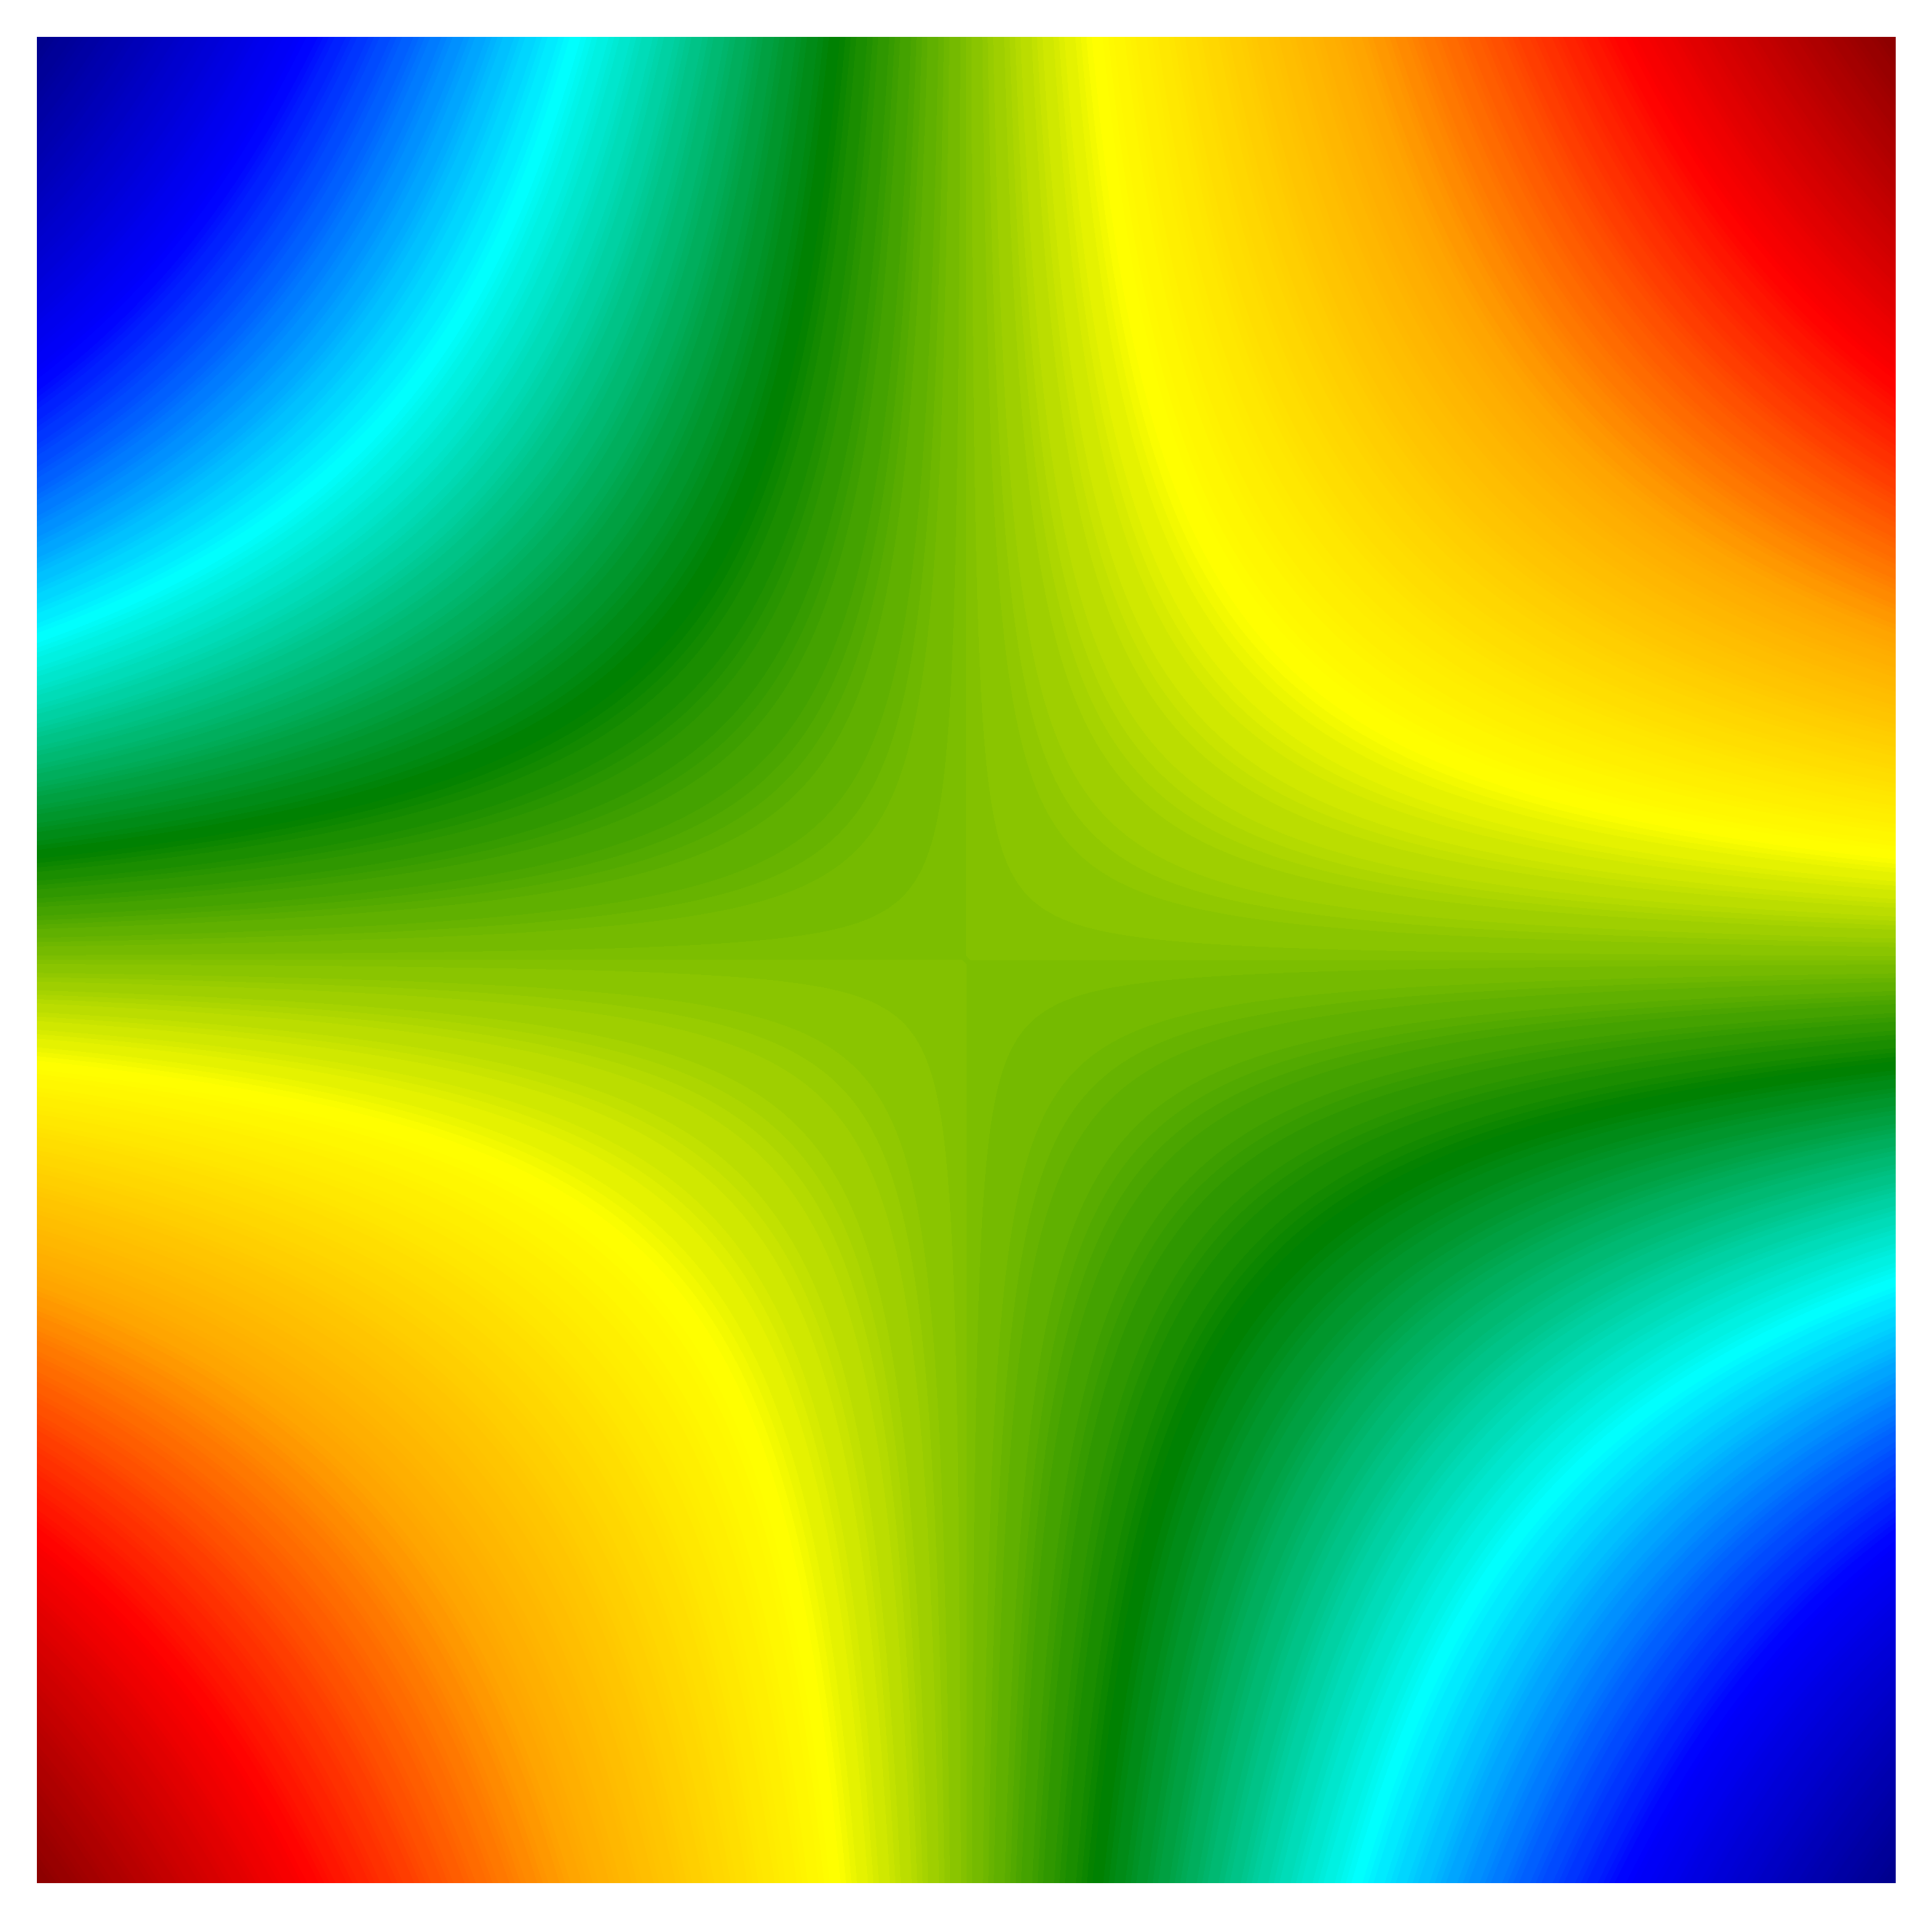
\includegraphics[width=\textwidth]{figs/FFFF1.png}
		\caption[]%
		{{\small }}    
		\label{fig:FFF1}
	\end{subfigure}
	\hfill
	\begin{subfigure}[b]{0.49\textwidth}  
		\centering 
		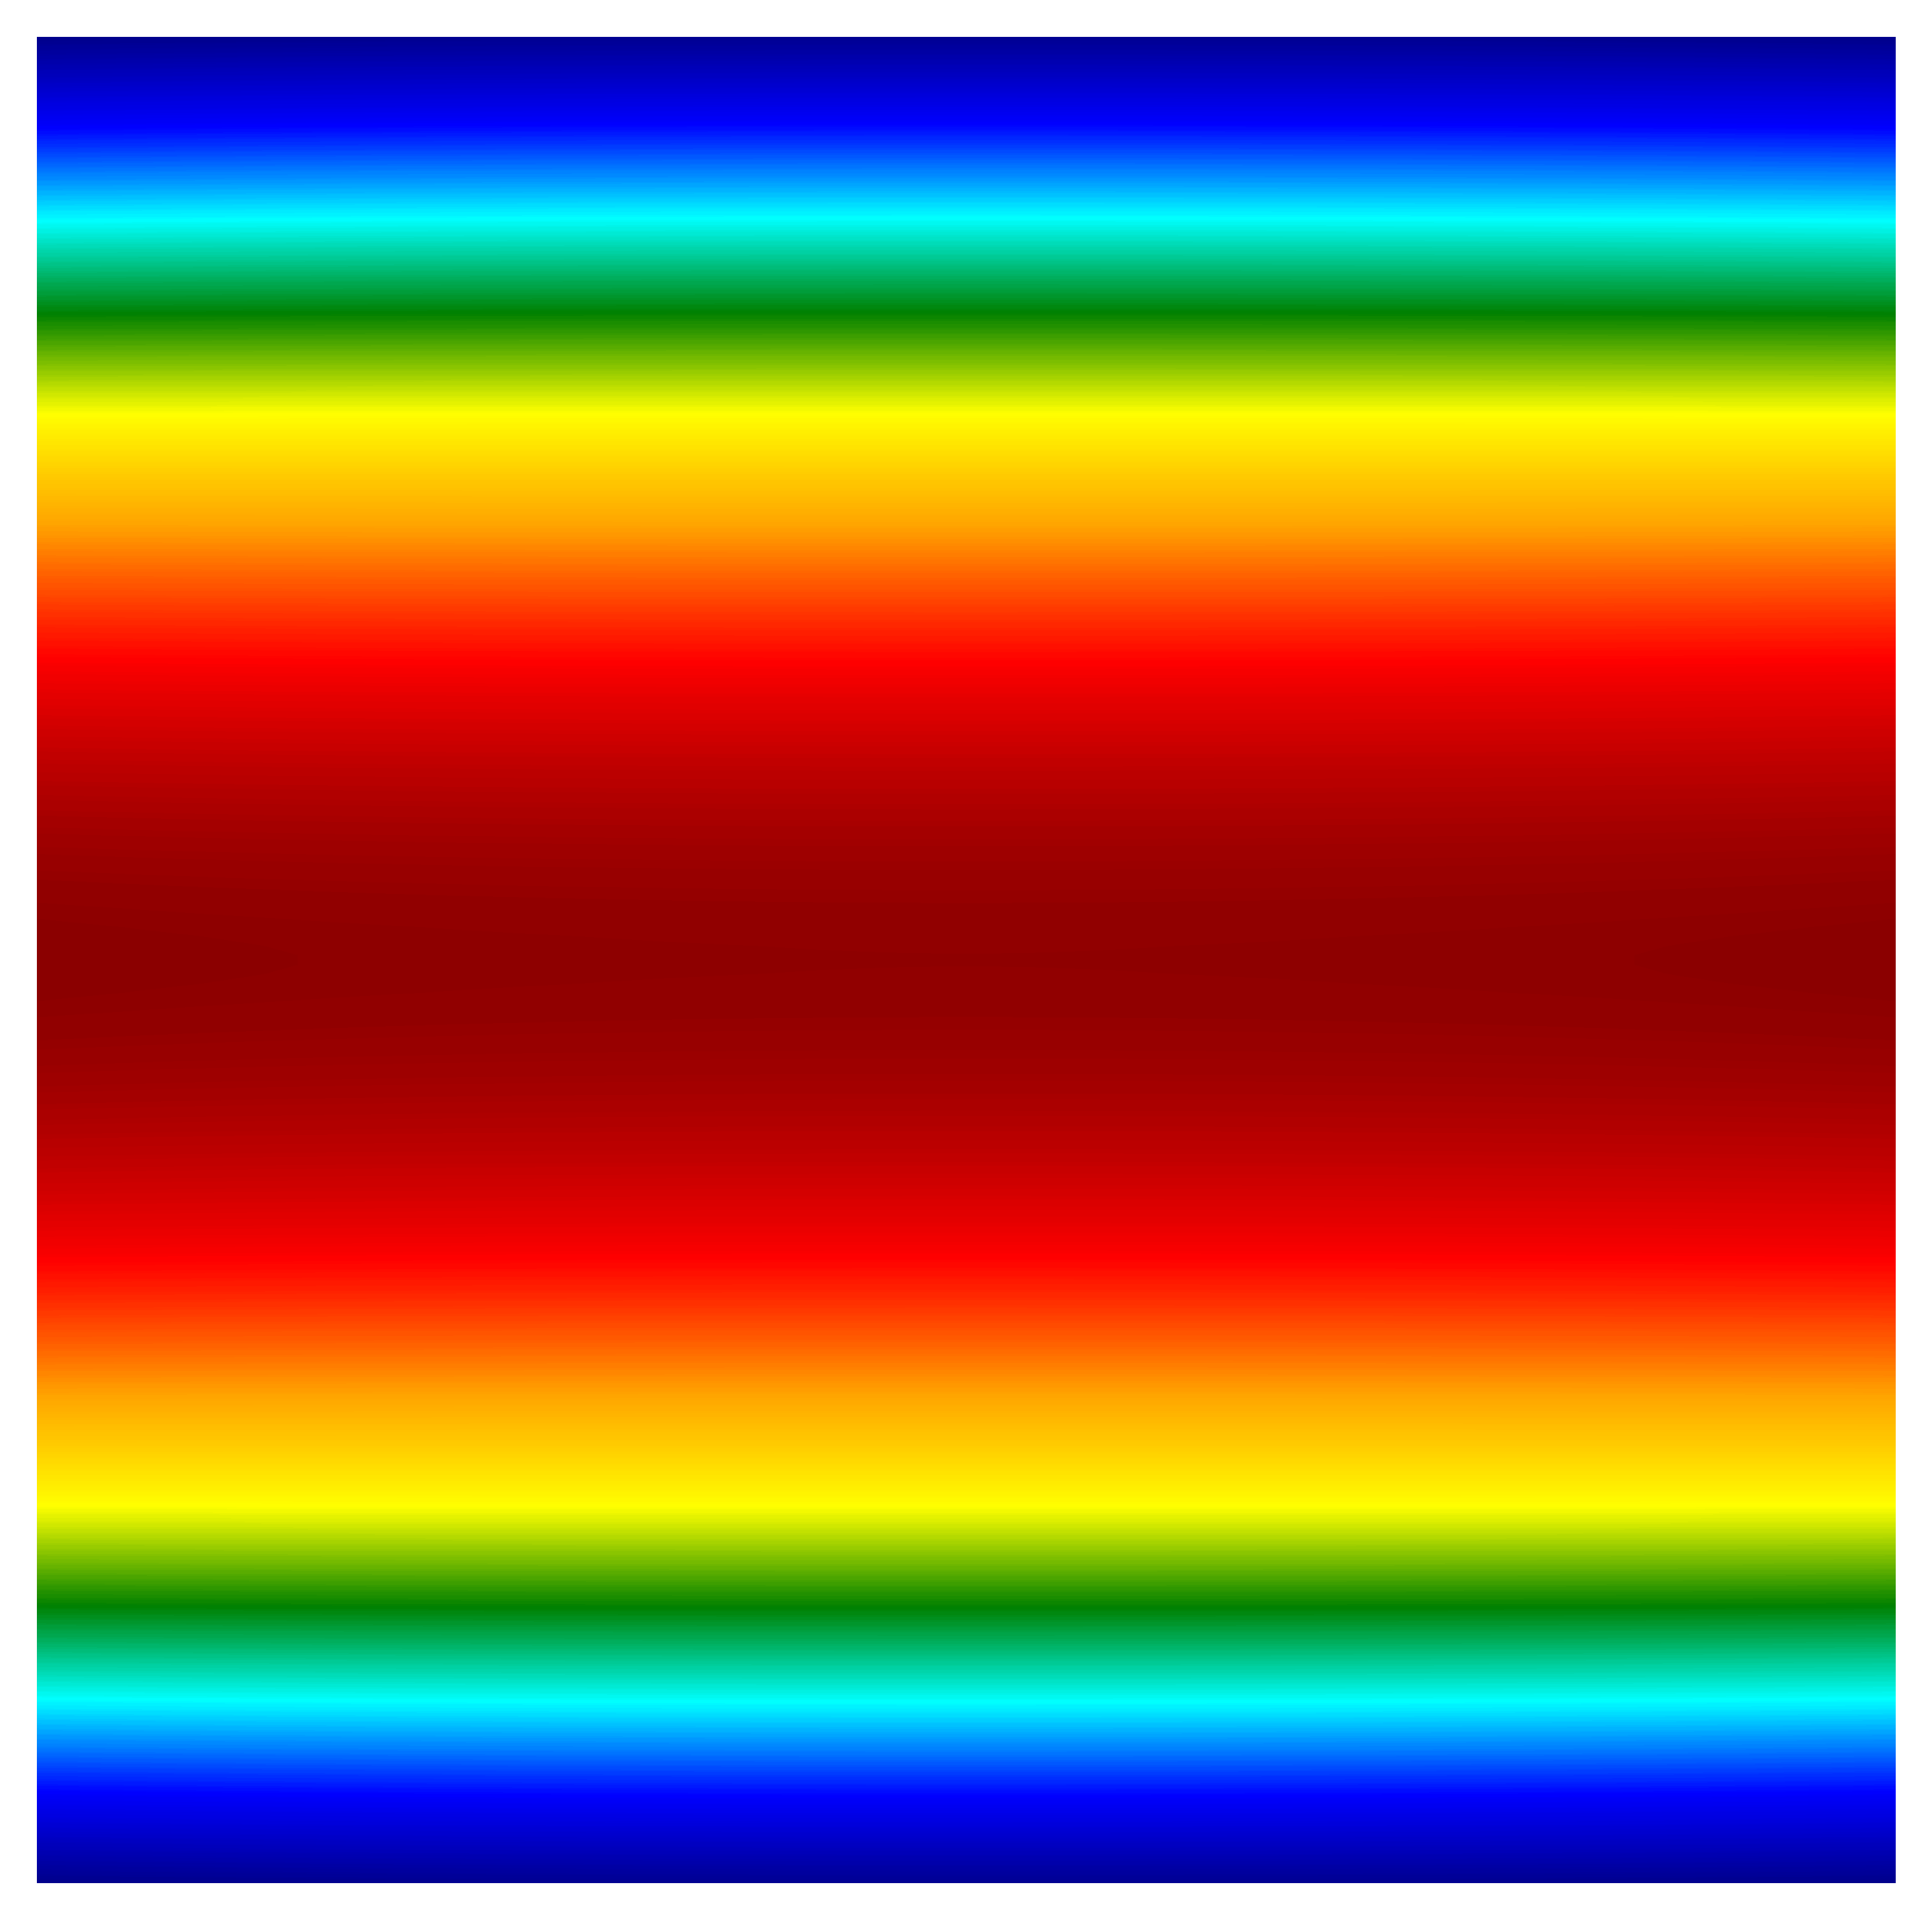
\includegraphics[width=\textwidth]{figs/FFFF2.png}
		\caption[]%
		{{\small }}    
		\label{fig:FFF2}
	\end{subfigure}
	\vfill
	\begin{subfigure}[b]{0.49\textwidth}   
		\centering 
		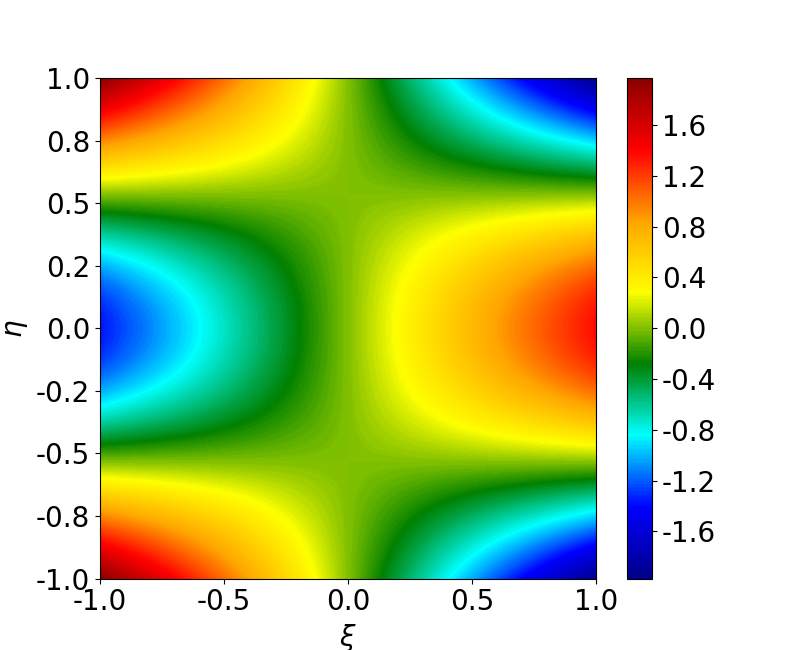
\includegraphics[width=\textwidth]{figs/FFFF3.png}
		\caption[]%
		{{\small }}    
		\label{fig:FFF3}
	\end{subfigure}
	\hfill
	\begin{subfigure}[b]{0.49\textwidth}   
		\centering 
		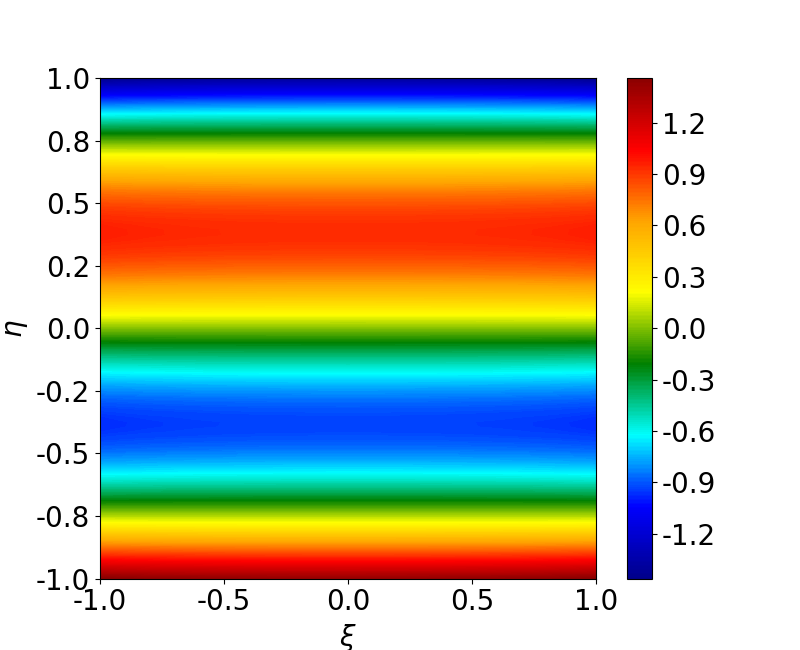
\includegraphics[width=\textwidth]{figs/FFFF4.png}
		\caption[]%
		{{\small }}    
		\label{fig:FFF4}
	\end{subfigure}
	\vskip\baselineskip
	\begin{subfigure}[b]{0.49\textwidth}   
		\centering 
		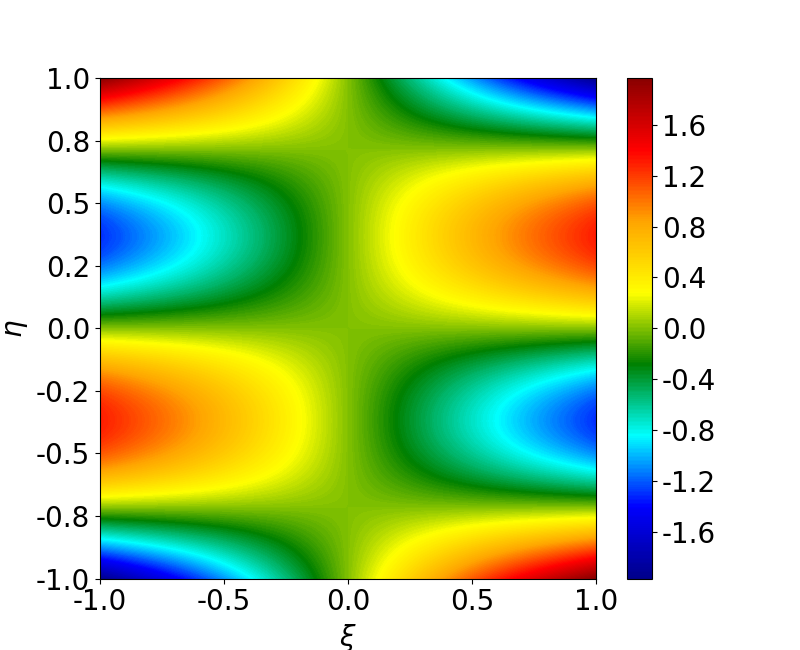
\includegraphics[width=\textwidth]{figs/FFFF5.png}
		\caption[]%
		{{\small}}    
		\label{fig:FFF5}
	\end{subfigure}
	\hfill
	\begin{subfigure}[b]{0.49\textwidth}   
		\centering 
		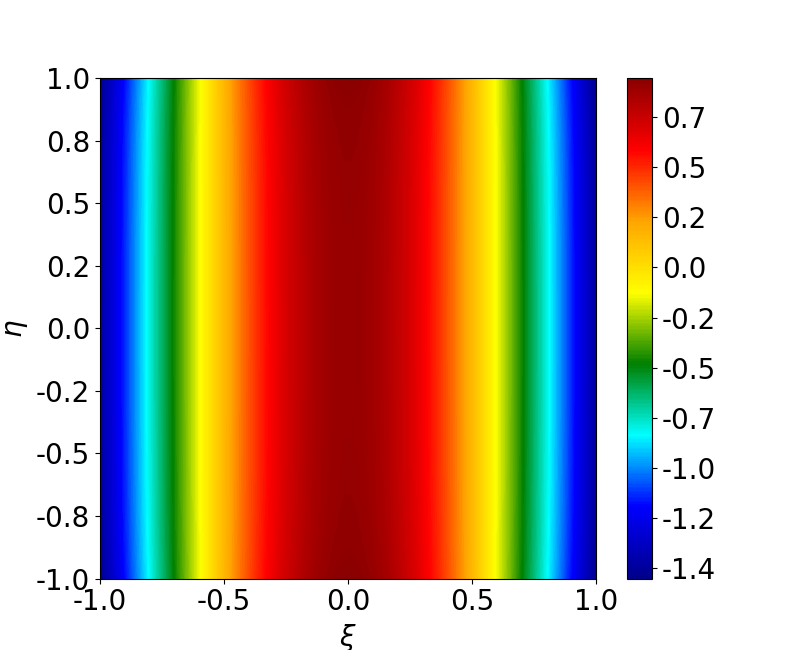
\includegraphics[width=\textwidth]{figs/FFFF6.png}
		\caption[]%
		{{\small }}    
		\label{fig:FFF6}
	\end{subfigure}
	\caption[]  
	{\small The first six nonzero mode shapes of a square orthotropic plate with FFFF boundary conditions: (a) the first mode; (b) the second mode; (c) the third mode; (d) the fourth mode; (e) the fifth mode; (f) the sixth mode.}  
	\label{fig:FFFF}
\end{figure}


\begin{table}[!htbp] 
	\centering
	\caption{The first seven frequency parameter $2a\Omega$ of of orthotropic rectangular plates with SSSS, SCSF and GCGC boundary conditions.}
	\begin{tabular}{c c l c c c c c c c}
		\toprule
		\multicolumn{3}{c}{} & \multicolumn{7}{c}{$2a\Omega_x=2a\Omega_y=2a\sqrt[4]{\rho h \omega^2/D_{11}}$} \\ 
		\cmidrule(lr){4-10}
		BCs & $\alpha$ & Mode & 1 & 2 & 3 & 4 & 5 & 6 & 7 \\
		\midrule
		SSSS & 0.5 & Mode number  & (1,1) & (1,2) & (1,3) & (1,4) & (1,5) & (1,6) & (1,7) \\
		&     & extended SOV \Citealp{xing2020extended}   & 3.1807 & 3.3190 & 3.5938 & 4.0135 & 4.5495 & 5.1635 & 5.8265 \\
		&     & Present       & 3.1825 & 3.3225 & 3.5975 & 4.0175 & 4.5525 & 5.1625 & 5.8275 \\
		& 1   & Mode number  & (1,1) & (1,2) & (1,3) & (2,1) & (1,4) & (2,2) & (2,3) \\
		&     & extended SOV \Citealp{xing2020extended}   & 3.3190 & 4.0135 & 5.1635 & 6.3615 & 6.5200 & 6.6379 & 7.1876 \\
		&     & Present       & 3.3175 & 4.0175 & 5.1625 & 6.3625 & 6.5175 & 6.6375 & 7.1875 \\
		& 1.5 & Mode number  & (1,1) & (1,2) & (2,1) & (2,2) & (1,3) & (2,3) & (1,4) \\
		&     & extended SOV \Citealp{xing2020extended}   & 3.5938 & 5.1635 & 6.4698 & 7.1876 & 7.2331 & 8.5389 & 9.4352 \\
		&     & Present       & 3.5975 & 5.1675 & 6.4725 & 7.1875 & 7.2325 & 8.5375 & 9.4375 \\
		SCSF & 0.5 & Mode number  & (1,1) & (1,2) & (1,3) & (1,4) & (1,5) & (1,6) & (1,7) \\
		&     & extended SOV \Citealp{xing2020extended}   & 3.1516 & 3.2451 & 3.4588 & 3.8131 & 4.2950 & 4.8711 & 5.5087 \\
		&     & Present      & 3.1525 & 3.2475 & 3.4575 & 3.8175 & 4.2925 & 4.8725 & 5.5075 \\
		& 1   & Mode number  & (1,1) & (1,2) & (1,3) & (1,4) & (2,1) & (2,2) & (2,3) \\
		&     & extended SOV \Citealp{xing2020extended}  & 3.1908 & 3.6428 & 4.5972 & 5.8599 & 6.3033 & 6.4901 & 6.9177 \\
		&     & Present        & 3.1925 & 3.6425 & 4.5975 & 5.8575 & 6.3025 & 6.4925 & 6.9175 \\
		& 1.5 & Mode number & (1,1) & (1,2) & (1,3) & (2,1) & (2,2) & (2,3) & (1,4) \\
		&     & extended SOV \Citealp{xing2020extended}   & 3.2710 & 4.3430 & 6.2157 & 6.3337 & 6.8043 & 7.8718 & 8.3518 \\
		&     & Present      & 3.2725 & 4.3425 & 6.2175 & 6.3325 & 6.8025 & 7.8725 & 8.3525 \\
		GCGC & 0.5 & Mode number & (1,1) & (1,2) & (1,3) & (2,1) & (2,2) & (1,4) & (2,3) \\
		&     & extended SOV \Citealp{xing2020extended}   & 1.1544 & 1.9166 & 2.6835 & 3.1983 & 3.3890 & 3.4501 & 3.7372 \\
		&     & Present      & 1.1525 & 1.9175 & 2.6825 & 3.1975 & 3.3875 & 3.4525 & 3.7375 \\
		& 1   & Mode number  & (1,1) & (2,1) & (1,2) & (2,2) & (1,3) & (2,3) & (3,1) \\
		&     & extended SOV \Citealp{xing2020extended}   & 2.3087 & 3.4900 & 3.8331 & 4.4682 & 5.3669 & 5.7736 & 6.3967 \\
		&     & Present       & 2.3075 & 3.4875 & 3.8325 & 4.4675 & 5.3675 & 5.7725 & 6.3975 \\
		& 1.5 & Mode number  & (1,1) & (2,1) & (1,2) & (2,2) & (3,1) & (3,2) & (1,3) \\
		&     & extended SOV \Citealp{xing2020extended}   & 3.4631 & 4.1353 & 5.7497 & 6.0981 & 6.6049 & 7.6449 & 8.0504 \\
		&     & Present       & 3.4625 & 4.1325 & 5.7475 & 6.0975 & 6.6075 & 7.6425 & 8.0525 \\
		\bottomrule
	\end{tabular}
	\label{tab:sov1}
\end{table}
\begin{table}[!htbp] 
	\centering
	\caption{The first seven frequency parameter $2a\Omega$ of of orthotropic rectangular plates with CCCC, SSCC, SCCC and GGCC boundary conditions.}
	\begin{tabular}{c c l c c c c c c c}
		\toprule
		\multicolumn{3}{c}{} & \multicolumn{7}{c}{$2a\Omega_x=2a\Omega_y=2a\sqrt[4]{\rho h \omega^2/D_{11}}$} \\ 
		\cmidrule(lr){4-10}
		BCs & $\alpha$ & Mode & 1 & 2 & 3 & 4 & 5 & 6 & 7 \\
		\midrule
		CCCC & 0.5 & Mode number  & (1,1) & (1,2) & (1,3) & (1,4) & (1,5) & (1,6) & (1,7) \\
		&     & extended SOV \Citealp{xing2020extended}   & 4.7500 & 4.8208 & 4.9682 & 5.2177 & 5.5791 & 6.0430 & 6.5892 \\
		&     & Present       & 4.7475 & 4.8225 & 4.9725 & 5.2175 & 5.5825 & 6.0425 & 6.5875 \\
		& 1   & Mode number   & (1,1) & (1,2) & (1,3) & (1,4) & (2,1) & (2,2) & (2,3) \\
		&     & extended SOV \Citealp{xing2020extended}   & 4.8579 & 5.3546 & 6.2819 & 7.4972 & 7.9193 & 8.1490 & 8.6054 \\
		&     & Present       & 4.8575 & 5.3575 & 6.2875 & 7.4975 & 7.9175 & 8.1475 & 8.6075 \\
		& 1.5 & Mode number   & (1,1) & (1,2) & (2,1) & (1,3) & (2,2) & (2,3) & (1,4) \\
		&     & extended SOV \Citealp{xing2020extended}   & 5.1581 & 6.5412 & 8.0409 & 8.4945 & 8.7204 & 9.9793 & 10.6460 \\
		&     & Present       & 5.1575 & 6.5375 & 8.0425 & 8.4975 & 8.7175 & 9.9775 & 10.6425 \\
		SSCC & 0.5 & Mode number   & (1,1) & (1,2) & (1,3) & (1,4) & (1,5) & (1,6) & (1,7) \\
		&     & extended SOV \Citealp{xing2020extended}   & 3.9542 & 4.0520 & 4.2525 & 4.5785 & 5.0254 & 5.5682 & 6.1789 \\
		&     & Present       & 3.9575 & 4.0525 & 4.2475 & 4.5775 & 5.0225 & 5.5725 & 6.1825 \\
		& 1   & Mode number  & (1,1) & (1,2) & (1,3) & (1,4) & (2,1) & (2,2) & (2,3) \\
		&     & extended SOV \Citealp{xing2020extended}   & 4.0745 & 4.6606 & 5.7009 & 6.9940 & 7.1396 & 7.3894 & 7.8881 \\
		&     & Present       & 4.0775 & 4.6625 & 5.7025 & 6.9925 & 7.1375 & 7.3875 & 7.8875 \\
		& 1.5 & Mode number   & (1,1) & (1,2) & (2,1) & (1,3) & (2,2) & (2,3) & (1,4) \\
		&     & extended SOV \Citealp{xing2020extended}   & 4.3602 & 5.8384 & 7.2531 & 7.8560 & 7.9481 & 9.2515 & 10.0366 \\
		&     & Present       & 4.3625 & 5.8325 & 7.2525 & 7.8575 & 7.9525 & 9.2525 & 10.0325 \\
		SCCC & 0.5 & Mode number & (1,1) & (1,2) & (1,3) & (1,4) & (1,5) & (1,6) & (1,7) \\
		&     & extended SOV \Citealp{xing2020extended}   & 3.9596 & 4.0745 & 4.3027 & 4.6606 & 5.1361 & 5.7009 & 6.3271 \\
		&     & Present       & 3.9575 & 4.0725 & 4.3025 & 4.6625 & 5.1325 & 5.7025 & 6.3325 \\
		& 1   & Mode number  & (1,1) & (1,2) & (1,3) & (2,1) & (1,4) & (2,2) & (2,3) \\
		&     & extended SOV \Citealp{xing2020extended}   & 4.1349 & 4.8478 & 5.9805 & 7.1541 & 7.3192 & 7.4478 & 8.0121 \\
		&     & Present       & 4.1325 & 4.8475 & 5.9825 & 7.1525 & 7.3175 & 7.4475 & 8.0125 \\
		& 1.5 & Mode number  & (1,1) & (1,2) & (2,1) & (2,2) & (1,3) & (2,3) & (3,1) \\
		&     &extended SOV \Citealp{xing2020extended}  & 4.5824 & 6.2766 & 7.3116 & 8.1528 & 8.3705 & 9.5986 & 10.3507 \\
		&     & Present       & 4.5825 & 6.2775 & 7.3125 & 8.1525 & 8.3725 & 9.5975 & 10.3525 \\
		GGCC & 0.5 & Mode number  & (1,1) & (1,2) & (1,3) & (1,4) & (1,5) & (1,6) & (1,7) \\
		&     & extended SOV \Citealp{xing2020extended}   & 2.3750 & 2.4841 & 2.7895 & 3.2946 & 3.9226 & 4.6123 & 5.3326 \\
		&     & Present       & 2.3725 & 2.4875 & 2.7925 & 3.2975 & 3.9225 & 4.6075 & 5.3325 \\
		& 1   & Mode number  & (1,1) & (1,2) & (1,3) & (2,1) & (2,2) & (1,4) & (2,3) \\
		&     & extended SOV \Citealp{xing2020extended}   & 2.4290 & 3.1410 & 4.4293 & 5.5202 & 5.7315 & 5.8801 & 6.2606 \\
		&     & Present       & 2.4325 & 3.1425 & 4.4325 & 5.5225 & 5.7325 & 5.8775 & 6.2625 \\
		& 1.5 & Mode number  & (1,1) & (1,2) & (2,1) & (2,2) & (1,3) & (2,3) & (3,1) \\
		&     & extended SOV \Citealp{xing2020extended}   & 2.5790 & 4.2472 & 5.5565 & 6.1533 & 6.4347 & 7.5231 & 8.6732 \\
		&     & Present       & 2.5825 & 4.2475 & 5.5575 & 6.1525 & 6.4325 & 7.5225 & 8.6725 \\
		\bottomrule
	\end{tabular}
	\label{tab:sov2}
\end{table}

\begin{table}[!htbp] 
	\centering
	\caption{The first seven nonzero frequency parameter $2a\Omega$ of of orthotropic rectangular plates with CCFF, CFCF, CFFF and FFFF boundary conditions.}
	\begin{tabular}{c c l c c c c c c c}
		\toprule
		\multicolumn{3}{c}{} & \multicolumn{7}{c}{$2a\Omega_x=2a\Omega_y=2a\sqrt[4]{\rho h \omega^2/D_{11}}$} \\ 
		\cmidrule(lr){4-10}
		BCs & $\alpha$ & Mode & 1 & 2 & 3 & 4 & 5 & 6 & 7 \\
		\midrule
		CCFF & 0.5 & Mode number   & (1,1) & (1,2) & (1,3) & (1,4) & (1,5) & (1,6) & (2,1) \\
		&     & extended SOV \Citealp{xing2020extended}   & 1.8978 & 2.0905 & 2.4925 & 3.0563 & 3.7110 & 4.4117 & 4.7029 \\
		&     & Present       & 1.8975 & 2.0925 & 2.4925 & 3.0575 & 3.7125 & 4.4125 & 4.7025 \\
		& 1   & Mode number  & (1,1) & (1,2) & (1,3) & (2,1) & (2,2) & (1,4) & (2,3) \\
		&     & extended SOV \Citealp{xing2020extended}   & 1.9930 & 2.7895 & 4.0733 & 4.7338 & 5.0652 & 5.5128 & 5.7419 \\
		&     & Present       & 1.9925 & 2.7875 & 4.0725 & 4.7325 & 5.0675 & 5.5125 & 5.7425 \\
		& 1.5 & Mode number  & (1,1) & (1,2) & (2,1) & (2,2) & (1,3) & (2,3) & (3,1) \\
		&     & extended SOV \Citealp{xing2020extended}   & 2.1780 & 3.7411 & 4.7931 & 5.5758 & 5.8895 & 7.0263 & 7.9006 \\
		&     & Present       & 2.1775 & 3.7425 & 4.7925 & 5.5725 & 5.8875 & 7.0275 & 7.9025 \\
		CFCF & 0.5 & Mode number   & (1,1) & (1,2) & (1,3) & (1,4) & (1,5) & (1,6) & (1,7) \\
		&     & extended SOV \Citealp{xing2020extended}   & 4.7297 & 4.7427 & 4.7881 & 4.8819 & 5.0478 & 5.3072 & 5.6694 \\
		&     & Present       & 4.7275 & 4.7425 & 4.7875 & 4.8825 & 5.0475 & 5.3075 & 5.6675 \\
		& 1   & Mode number  & (1,1) & (1,2) & (1,3) & (1,4) & (1,5) & (1,6) & (2,1) \\
		&     & extended SOV \Citealp{xing2020extended}   & 4.7295 & 4.7817 & 5.0012 & 5.5348 & 6.4407 & 7.6182 & 7.8523 \\
		&     & Present       & 4.7275 & 4.7825 & 5.0025 & 5.5325 & 6.4425 & 7.6175 & 7.8525 \\
		& 1.5 & Mode number  &(1,1) & (1,2) & (1,3) & (1,4) & (2,1) & (2,2) & (2,3) \\
		&     & extended SOV \Citealp{xing2020extended}   & 4.7292 & 4.8458 & 5.4221 & 6.7635 & 7.8518 & 7.9470 & 8.3021 \\
		&     & Present       & 4.7275 & 4.8475 & 5.4225 & 6.7625 & 7.8525 & 7.9475 & 8.3025 \\
		CFFF & 0.5 & Mode number   & (1,1) & (1,2) & (1,3) & (1,4) & (1,5) & (1,6) & (1,7) \\
		&     & extended SOV \Citealp{xing2020extended}   & 1.8751 & 1.9439 & 2.1679 & 2.5657 & 3.1106 & 3.7486 & 4.4382 \\
		&     & Present       & 1.8775 & 1.9425 & 2.1675 & 2.5675 & 3.1125 & 3.7475 & 4.4375 \\
		& 1   & Mode number  &(1,1) & (1,2) & (1,3) & (1,4) & (2,1) & (2,2) & (2,3) \\
		&     & extended SOV \Citealp{xing2020extended}   & 1.8750 & 2.1242 & 2.9077 & 4.1319 & 4.6937 & 4.8226 & 5.2263 \\
		&     & Present       & 1.8775 & 2.1225 & 2.9075 & 4.1325 & 4.6925 & 4.8225 & 5.2275 \\
		& 1.5 & Mode number  &(1,1) & (1,2) & (1,3) & (2,1) & (2,2) & (2,3) & (1,4) \\
		&     & extended SOV \Citealp{xing2020extended}   & 1.8750 & 2.3402 & 3.8522 & 4.6935 & 4.9753 & 5.8314 & 5.9292 \\
		&     & Present       & 1.8775 & 2.3425 & 3.8525 & 4.6925 & 4.9775 & 5.8325 & 5.9275 \\
		FFFF & 0.5 & Mode number  &(1,3) & (2,2) & (1,4) & (2,3) & (1,5) & (2,4) & (2,5) \\
		&     & extended SOV \Citealp{xing2020extended}   & 1.1540 & 1.4858 & 1.9157 & 2.1704 & 2.6821 & 2.7881 & 3.4093 \\
		&     & Present       & 1.1525 & 1.4875 & 1.9175 & 2.1725 & 2.6825 & 2.7875 & 3.4075 \\
		& 1   & Mode number  &(2,2) & (1,3) & (2,3) & (1,4) & (2,4) & (3,1) & (3,2) \\
		&     & extended SOV \Citealp{xing2020extended}   & 2.1311 & 2.3082 & 3.2734 & 3.8320 & 4.4962 & 4.7298 & 4.9138 \\
		&     & Present       & 2.1325 & 2.3075 & 3.2725 & 3.8325 & 4.4975 & 4.7275 & 4.9125 \\
		& 1.5 & Mode number  &(2,2) & (1,3) & (2,3) & (3,1) & (3,2) & (1,4) & (3,3) \\
		&     & extended SOV \Citealp{xing2020extended}   & 2.6277 & 3.4625 & 4.2915 & 4.7296 & 5.1259 & 5.7485 & 6.1588 \\
		&     & Present       & 2.6275 & 3.4625 & 4.2925 & 4.7275 & 5.1275 & 5.7475 & 6.1575 \\
		\bottomrule
	\end{tabular}
	\label{tab:sov3}
\end{table}
\subsection{Rotationally restrained boundary conditions}
In this subsection, rectangular orthotropic plates with rotationally restrained edges ($k^v_\xi = k^v_\eta = \infty$) are validated.  
The rotational stiffness coefficients are defined as: 
% 
\begin{subequations}\label{eq:rotation_coex}
	\begin{align}
		r_{\xi} &= \frac{2a k^r_{\xi}}{D_{11}}, \\
		r_{\eta} &= \frac{2b k^r_{\eta}}{D_{22}}.
	\end{align}
\end{subequations}


The first example considers a square isotropic plate with all four edges rotationally restrained. The vertical translational springs along the four edges are numerically set as $ k^v_{\xi=-1} = k^v_{\xi=1} = k^v_{\eta=-1} = k^v_{\eta=1} = 1 \times 10^{12} \ustif $. The material properties are given as $ D_{11} = D_{22} = D_3 $ and $ v_{12} = v_{21} = 0.3 $.  

\Cref{tab:rot1} presents the frequency parameter $2a\Omega $ for different rotational stiffness coefficients  $ r_{\xi} = r_{\eta} $ with values $ 0.1, 1, 10, 100, $ and $ 1000$.  
Notably, when $ r_{\xi} = r_{\eta} = 0 $ and $r_{\xi} = r_{\eta} = \infty$, the boundary conditions correspond to SSSS and CCCC, respectively.  

Interestingly, the results indicate that the frequencies $\Omega_x$ and $\Omega_y$ are not strictly equal for some mode shapes under rotationally restrained boundary conditions.  
The actual frequency $\Omega$ lies between $\Omega_x$ and $\Omega_y$, which may be attributed to the fact that $\Omega_x$ and $\Omega_y$ satisfy Rayleigh’s principle in \Cref{eq:Rayleigh}, representing the weak-form governing equations, but do not necessarily satisfy the strong-form governing equations in \Cref{eq:governing_EOM}.
For a physical problem with exact solutions, both \Cref{eq:Rayleigh,eq:governing_EOM} must be satisfied.  
If this condition is not met, applying \Cref{eq:Rayleigh} still provides a viable approach for approximating the exact solution of the plate.  
Thus, the exact frequency can be estimated as $\Omega = (\Omega_x + \Omega_y)/2$.  
As shown in \Cref{tab:rot1}, the maximum difference between \(\Omega\) and the solutions reported in \Citealp{zhang2019new} is less than $1.3\%$.
\Cref{fig:iso} illustrates the variation in mode shapes corresponding to the fundamental natural frequency as the rotational stiffness $r_{\xi} = r_{\eta}$ increases from zero to $\infty$, transitioning the boundary conditions from SSSS to CCCC.


\begin{figure}
	\centering
	\begin{subfigure}[b]{0.49\textwidth}
		\centering
		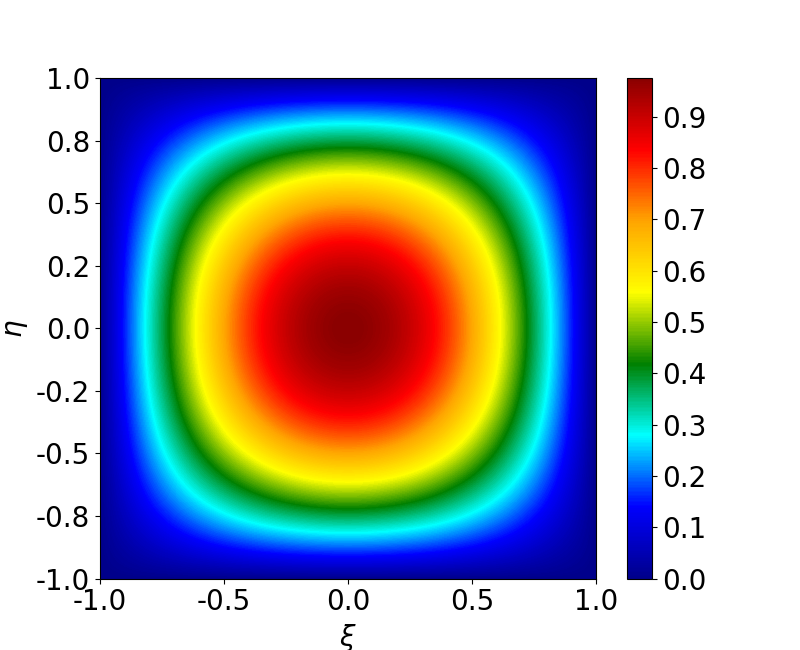
\includegraphics[width=\textwidth]{figs/iso0.png}
		\caption[]%
		{{\small }}    
		\label{fig:iso0}
	\end{subfigure}
	\hfill
	\begin{subfigure}[b]{0.49\textwidth}  
		\centering 
		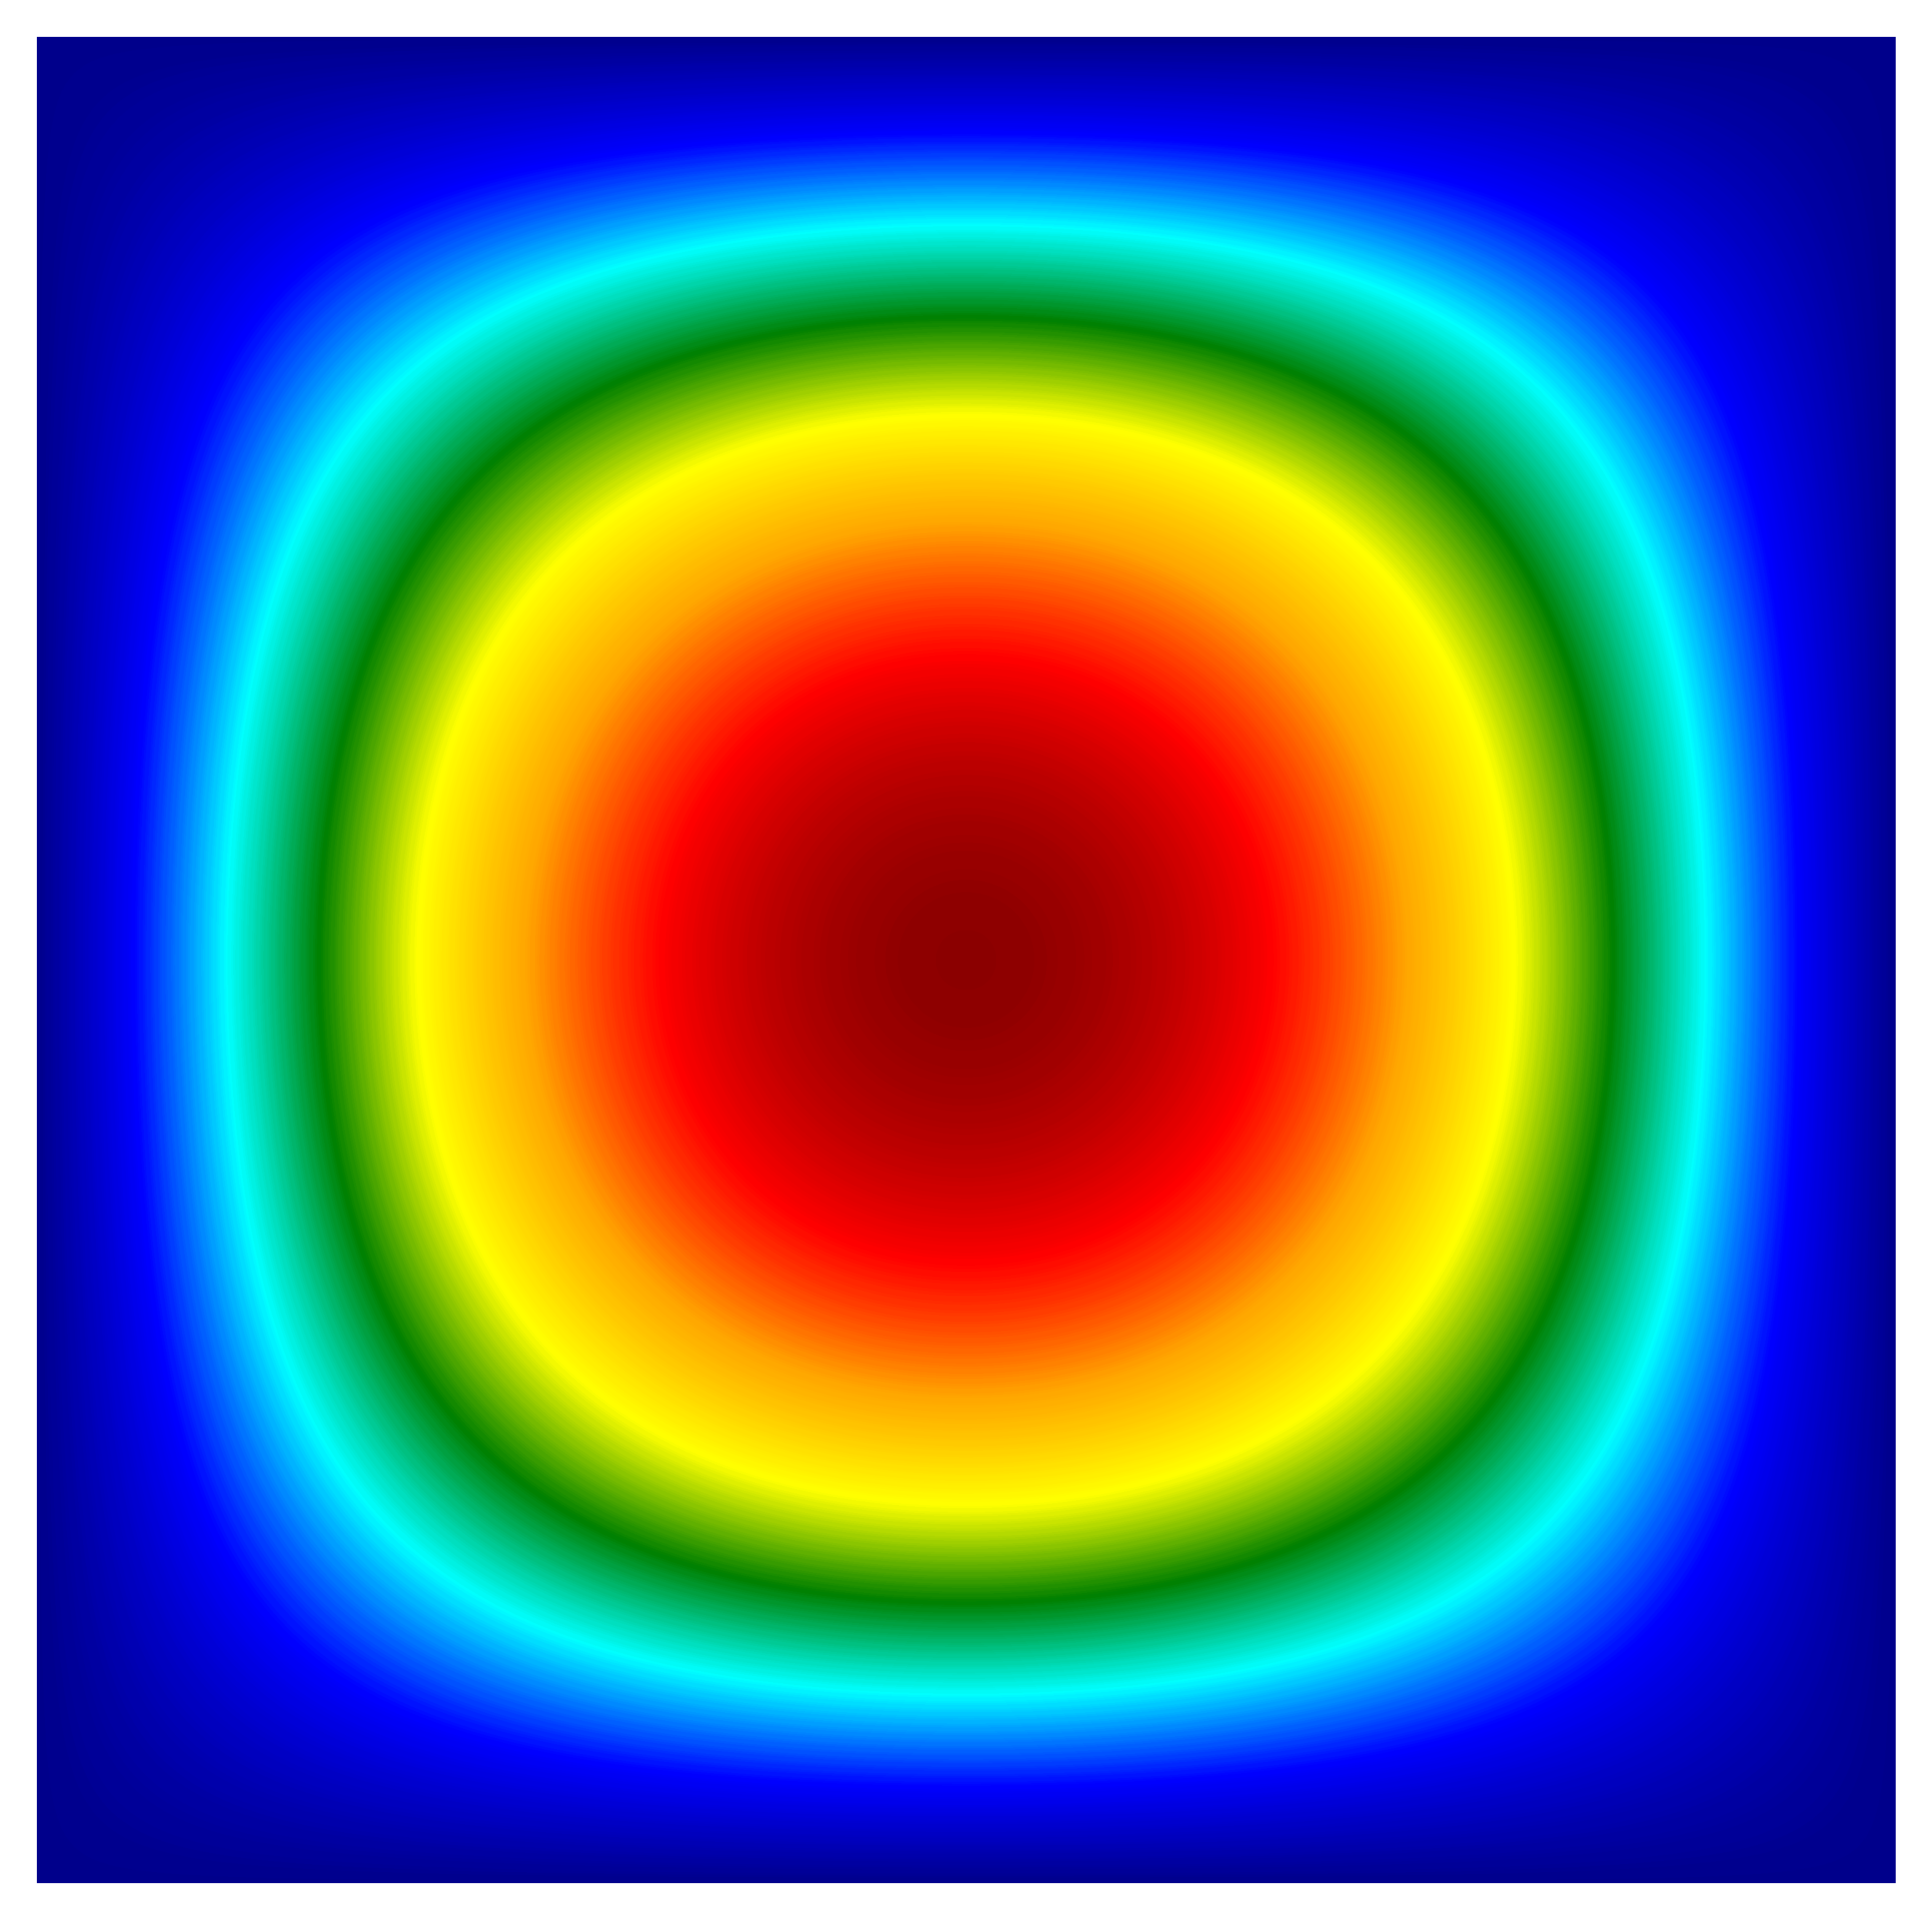
\includegraphics[width=\textwidth]{figs/iso1.png}
		\caption[]%
		{{\small }}    
		\label{fig:iso1}
	\end{subfigure}
	\vfill
	\begin{subfigure}[b]{0.49\textwidth}   
		\centering 
		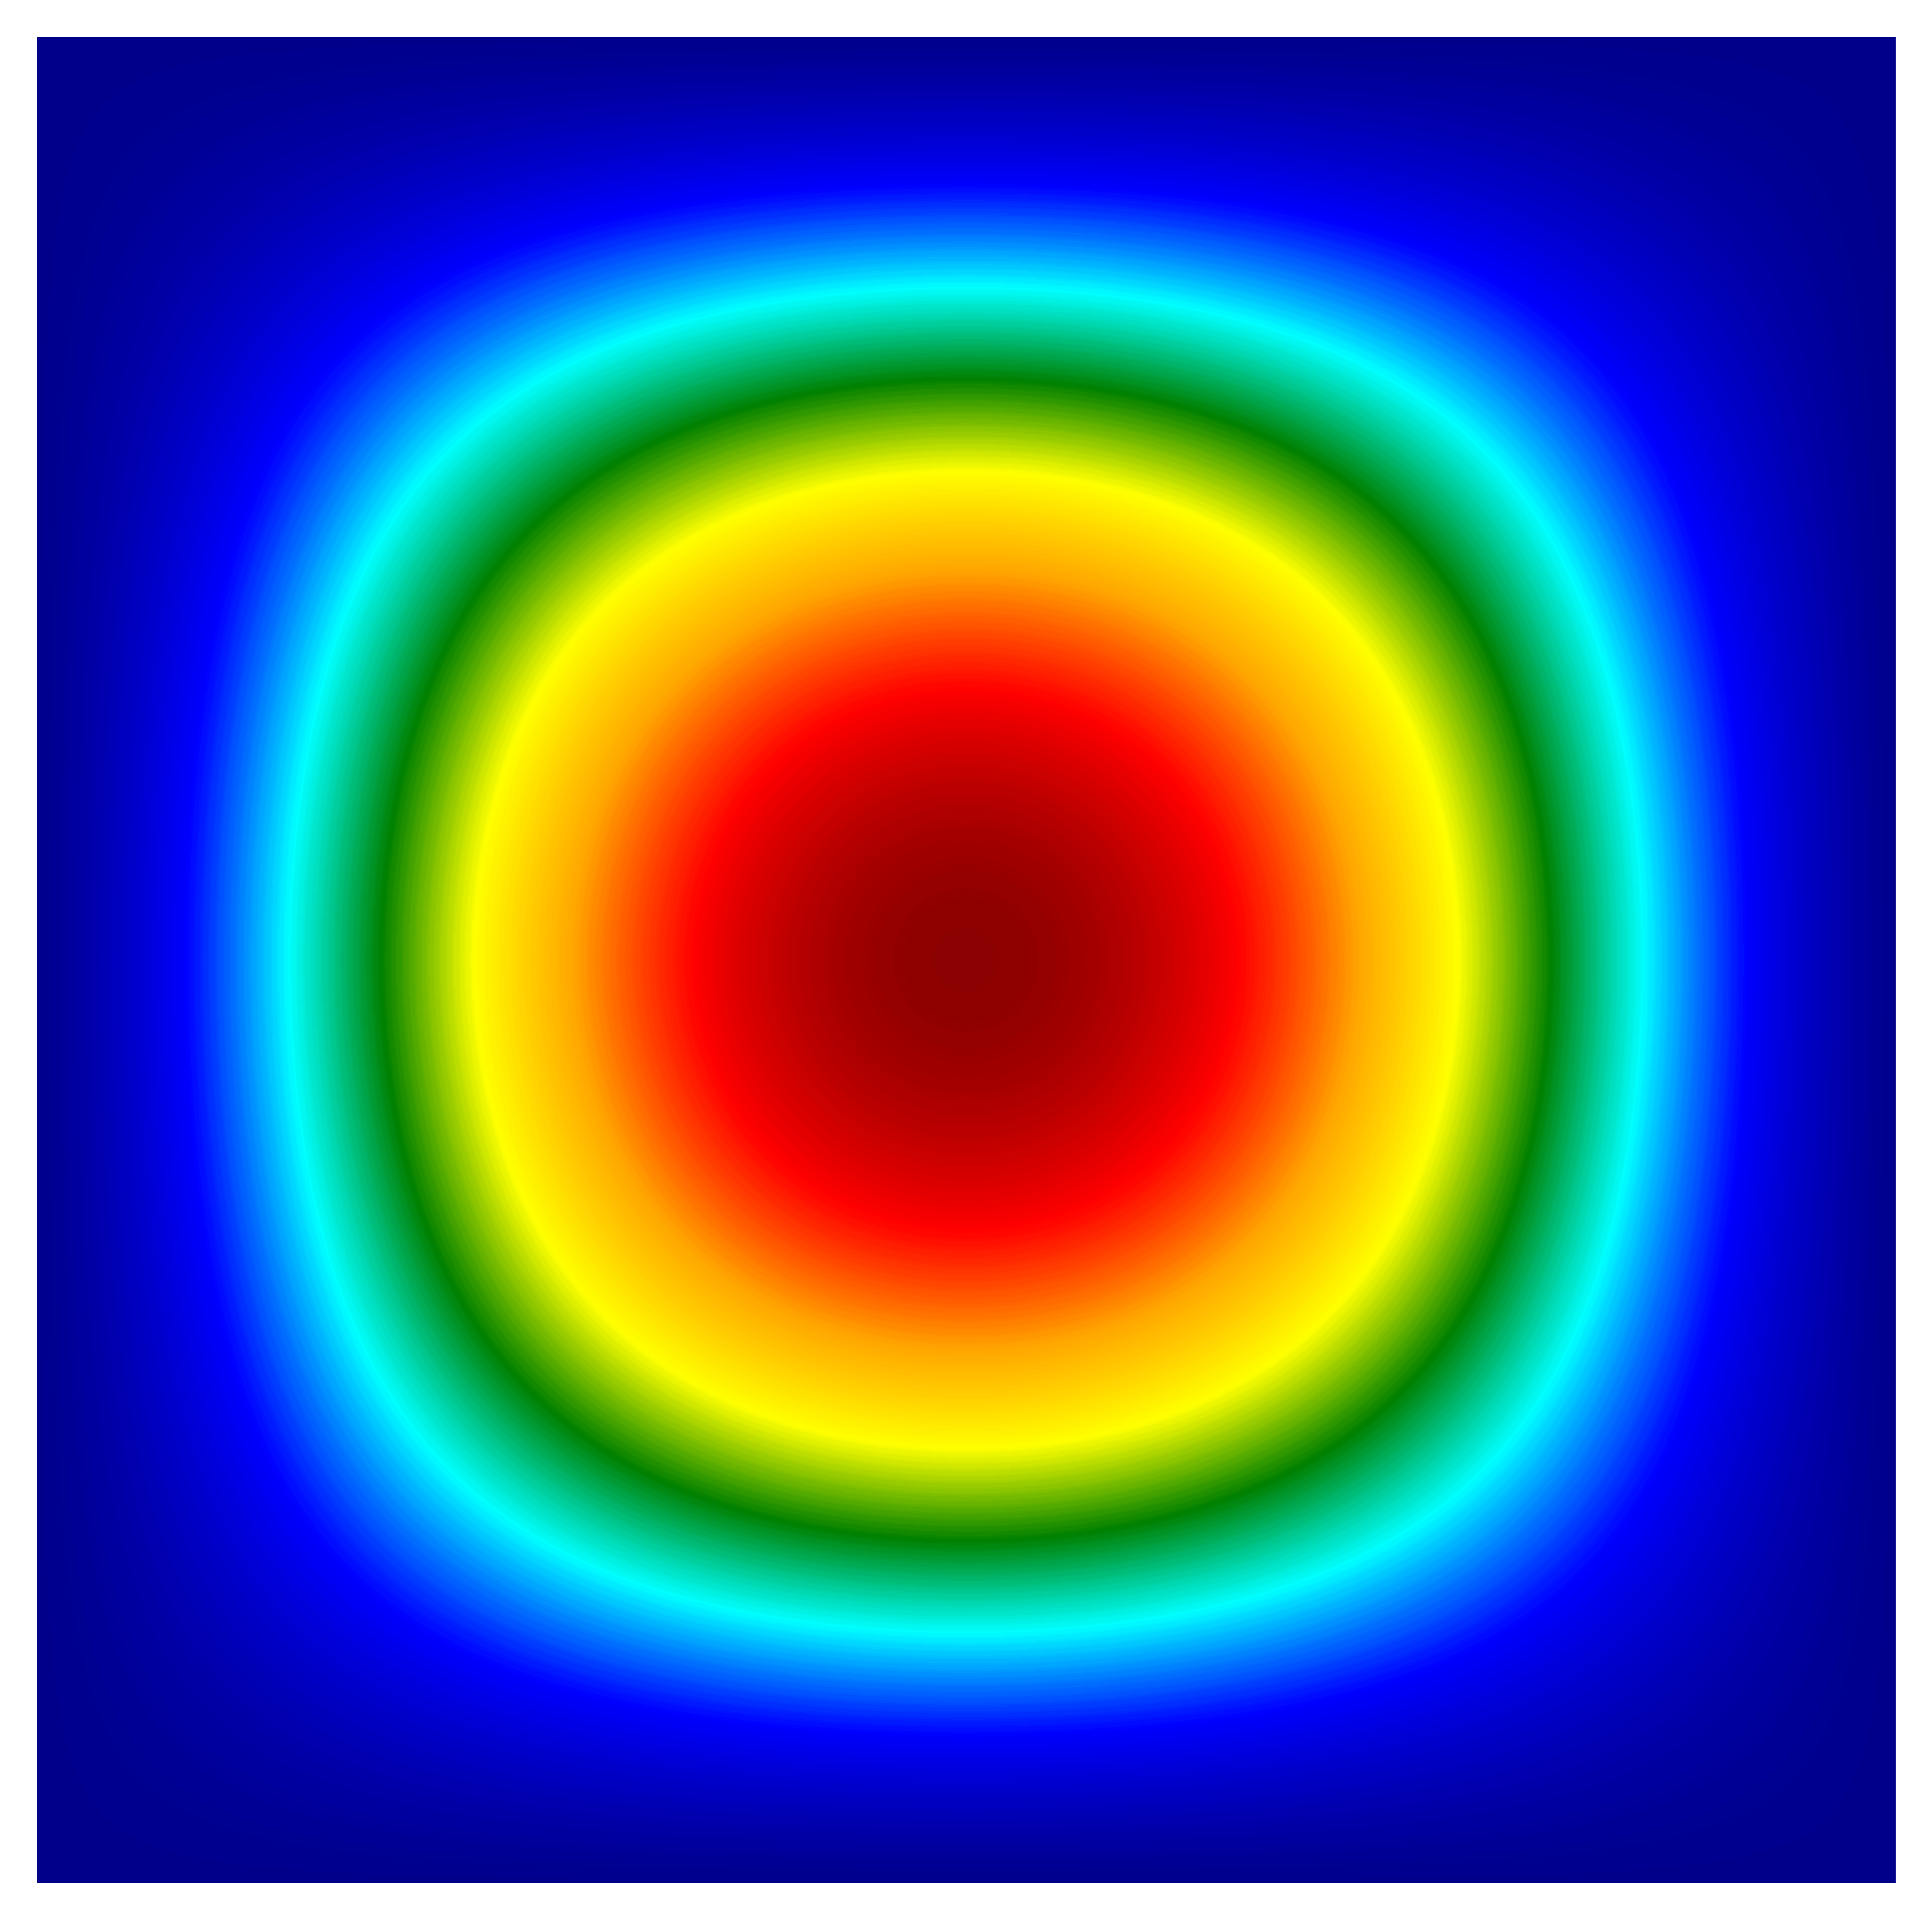
\includegraphics[width=\textwidth]{figs/iso10.png}
		\caption[]%
		{{\small }}    
		\label{fig:iso10}
	\end{subfigure}
	\hfill
	\begin{subfigure}[b]{0.49\textwidth}   
		\centering 
		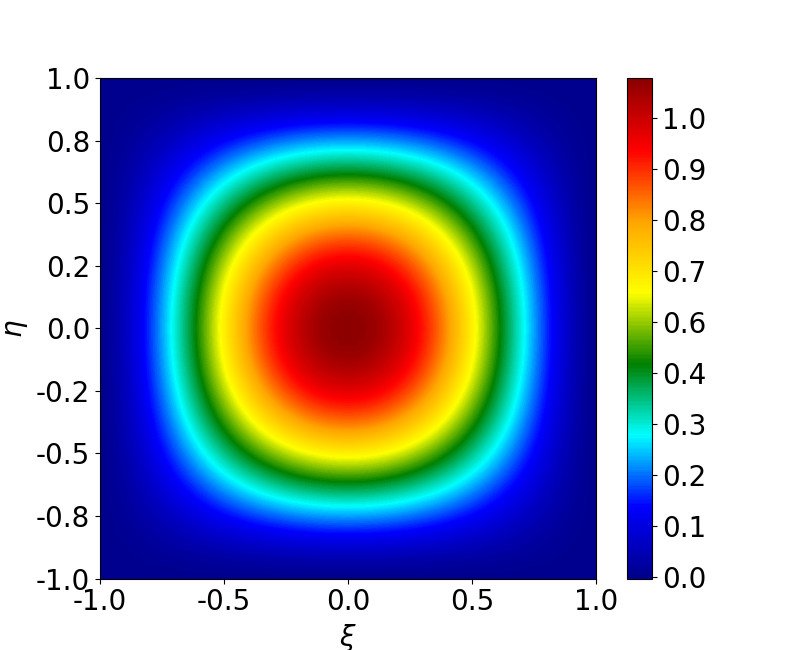
\includegraphics[width=\textwidth]{figs/iso20.png}
		\caption[]%
		{{\small }}    
		\label{fig:iso20}
	\end{subfigure}
	\vskip\baselineskip
	\begin{subfigure}[b]{0.49\textwidth}   
		\centering 
		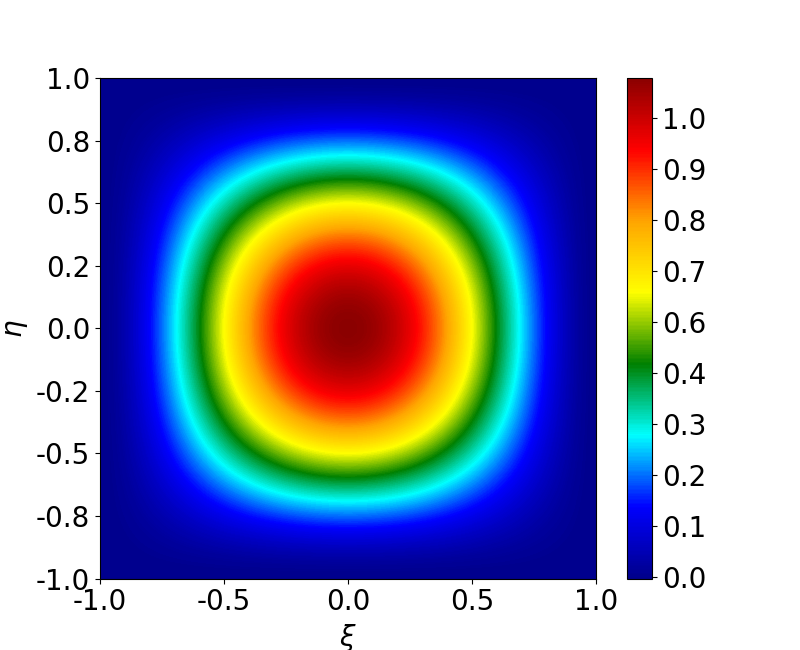
\includegraphics[width=\textwidth]{figs/iso100.png}
		\caption[]%
		{{\small}}    
		\label{fig:iso100}
	\end{subfigure}
	\hfill
	\begin{subfigure}[b]{0.49\textwidth}   
		\centering 
		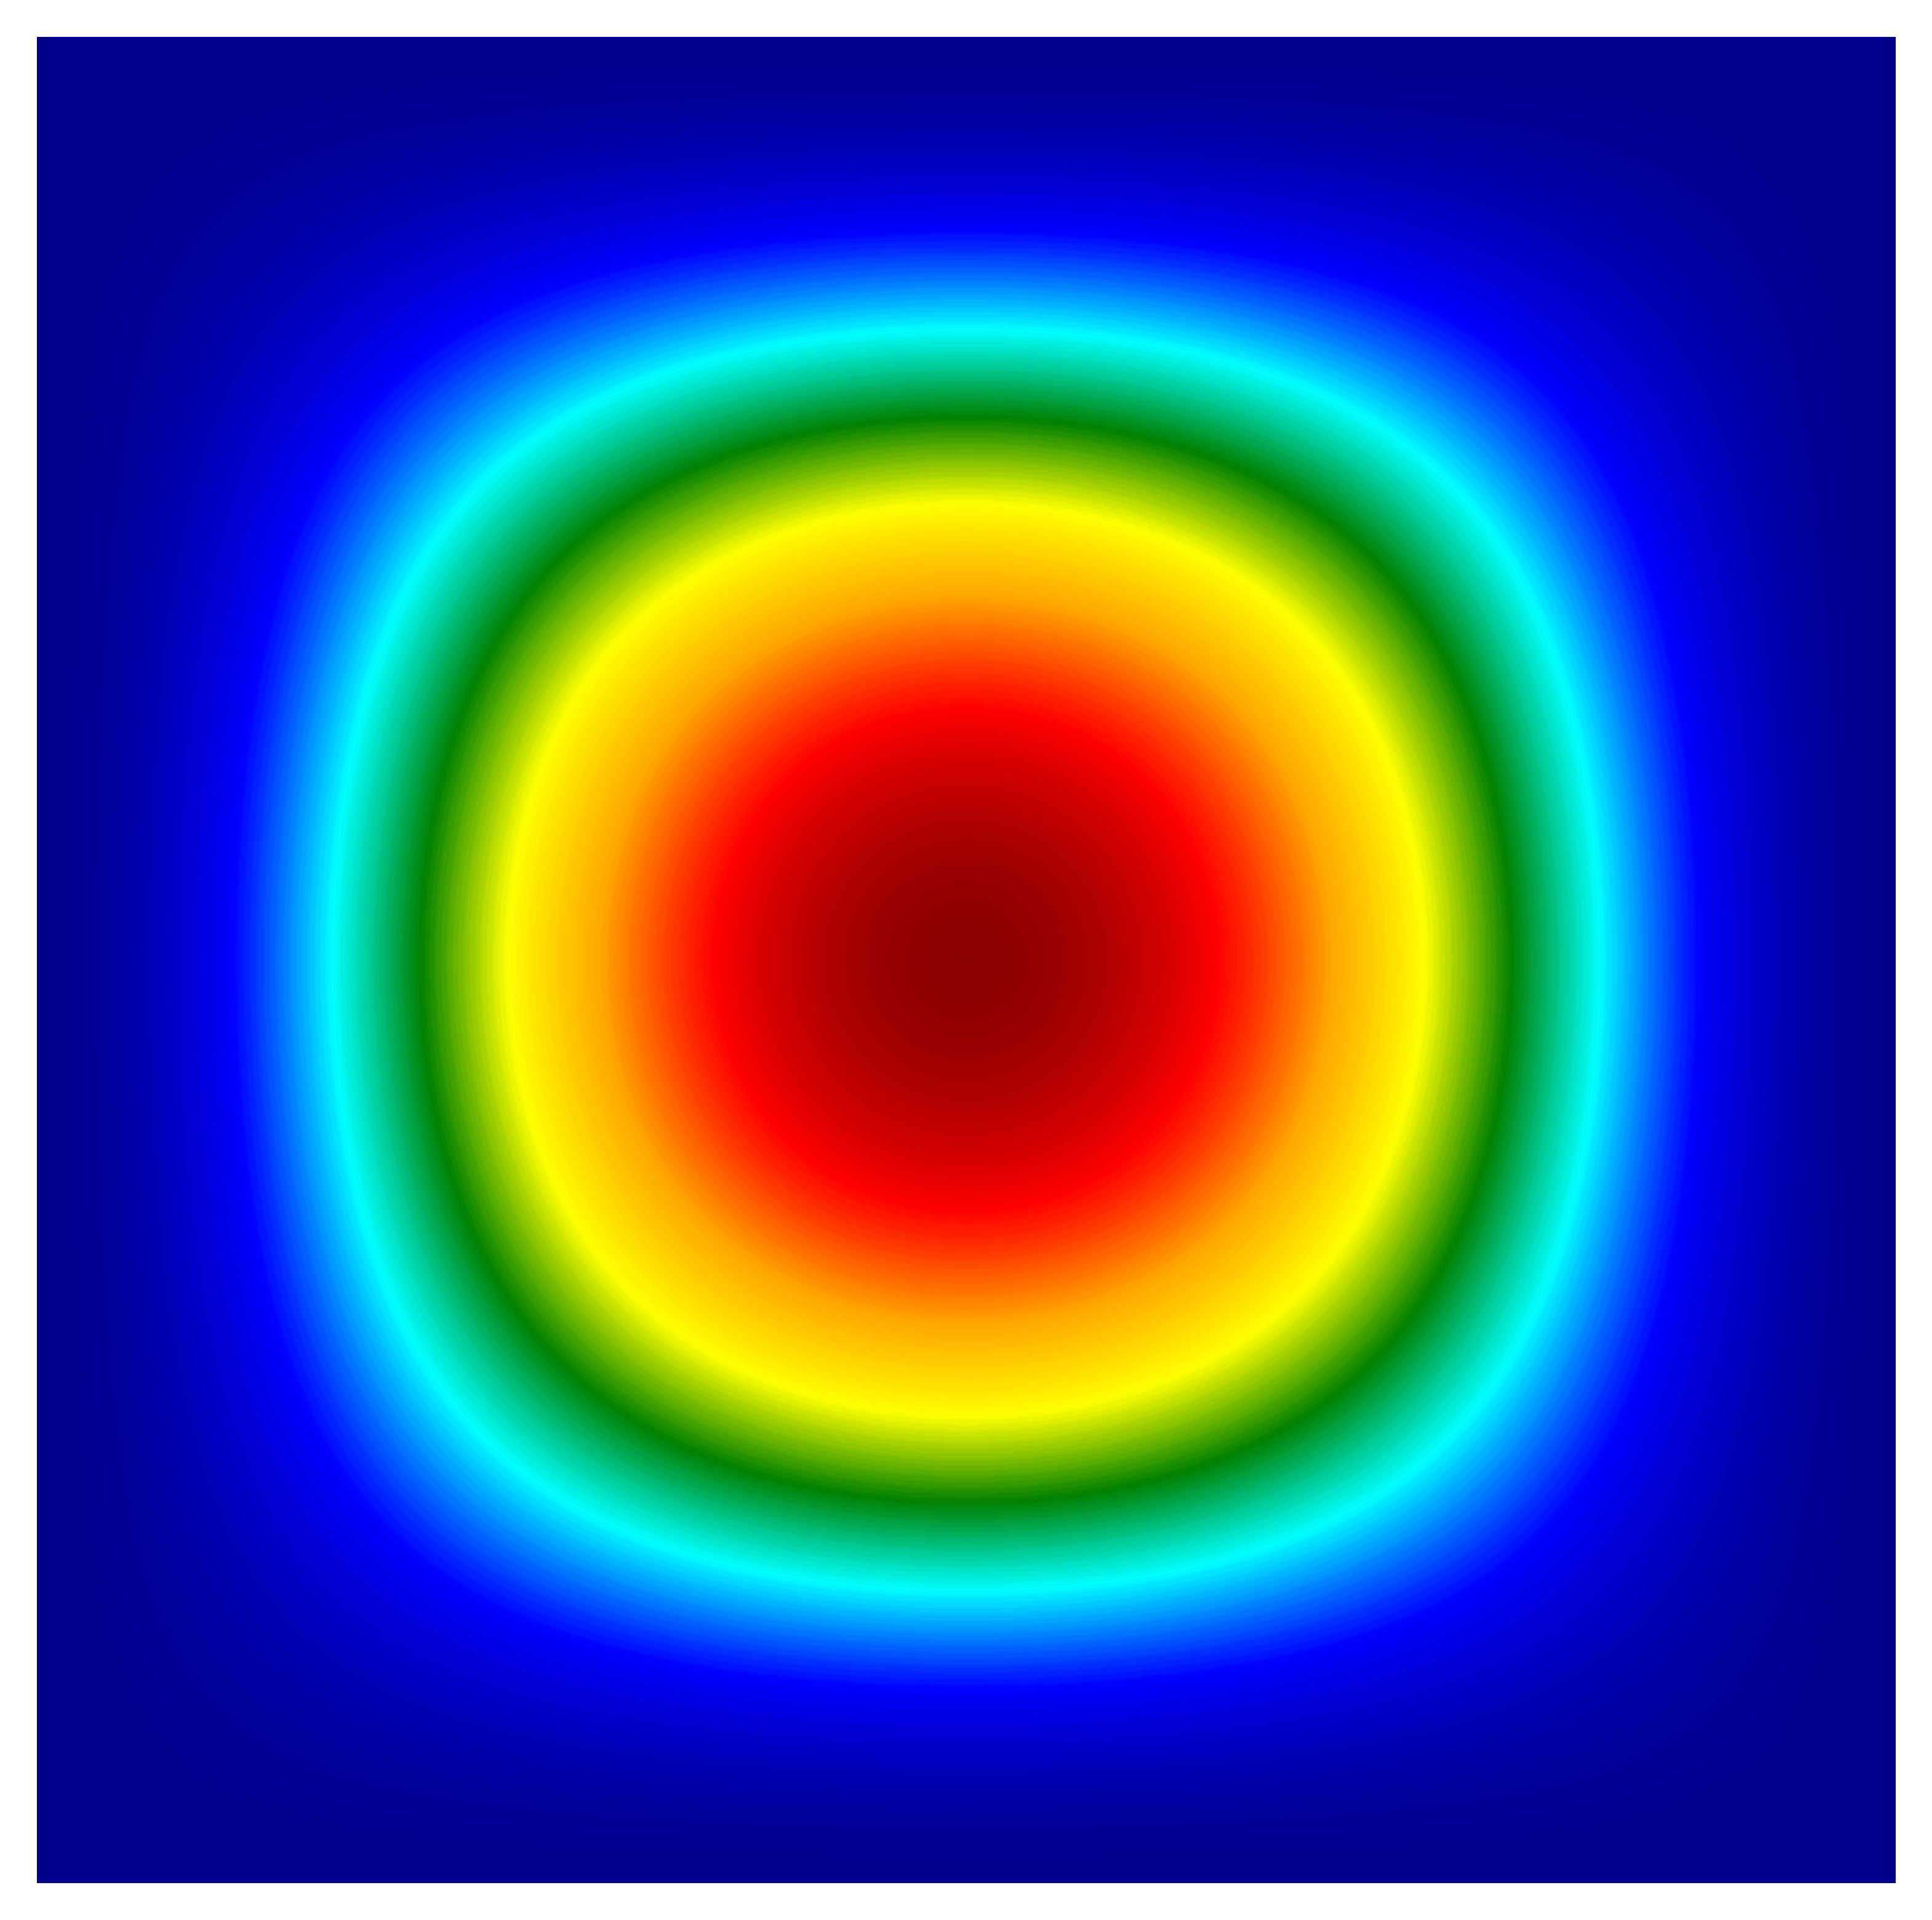
\includegraphics[width=\textwidth]{figs/isoinf.png}
		\caption[]%
		{{\small }}    
		\label{fig:isoinf}
	\end{subfigure}
	\caption[]  
	{\small The first mode shape of a square isotropic plate with all four edges rotationally restrained: (a) $r_{\xi} = r_{\eta} = 0$; (b) $r_{\xi} = r_{\eta} = 1$; (c) $r_{\xi} = r_{\eta} = 10$; (d) $r_{\xi} = r_{\eta} = 20$; (e) $r_{\xi} = r_{\eta} = 100$; (f) $r_{\xi} = r_{\eta} = \infty$.}  
	\label{fig:iso} 
\end{figure}

\begin{table}[!htbp]
	\centering
	\caption{The first six frequency parameters, $2a\Omega = 2a\sqrt[4]{\rho h \omega^2/D_{11}}$, of a square isotropic plate with all four edges rotationally restrained, where $k^r_{\xi=-1} = k^r_{\xi=1} = k^r_{\eta=-1} = k^r_{\eta=1}$.}
	\begin{tabular}{c l c c c c c c}
		\toprule
		\multicolumn{1}{c}{} & \multicolumn{6}{c}{$2a\Omega$} \\ 
		\cmidrule(lr){3-8}
		$r$ & Mode & 1 & 2 & 3 & 4 & 5 & 6 \\ 
		\midrule
		0.1 & Mode number   & (1,1) & (1,2) & (2,1) & (2,2) & (1,3) & (3,1) \\
		& Ref.\Citealp{mukhopadhyay1979free} & 4.454 & 6.992 & 7.045 & 8.890  & 9.782  & 9.960 \\
		& Ref.\Citealp{zhang2019new} & 4.465 & 7.039 & 7.039 &8.897  &9.945& 9.945 \\
		& Present ($\Omega_x$)   & 4.463     & 7.028     & 7.043     & 8.893     & 9.938       & 9.953  \\
		& Present ($\Omega_y$)   & 4.463    &7.043     &  7.028       & 8.893   &  9.953    & 9.938 \\ 
		& Present ($\Omega$)   & 4.463    & 7.035     & 7.035      &8.893     & 9.945     & 9.945   \\
		&Difference (\%)& 0.044     & 0.056      & 0.056      & 0.044     &  0.000     & 0.000
		\\
		\\
		1 & Mode number   &  (1,1) & (1,2) & (2,1) & (2,2) & (3,1) & (1,3) \\
		& Ref.\Citealp{mukhopadhyay1979free} & 4.529& 7.008 &7.136 &8.936& 9.787& 10.036 \\
		& Ref.\Citealp{zhang2019new} & 4.637 &7.155 & 7.155 & 8.991 & 10.029 & 10.030 \\
		& Present ($\Omega_x$)   & 4.648     & 7.098      &7.223     & 8.993     &   10.093    & 9.968  \\
		& Present ($\Omega_y$)   & 4.648     & 7.223     & 7.098       & 8.993     &   9.968     & 10.098
		\\ 
		& Present ($\Omega$)   & 4.648      & 7.160   & 7.160     & 8.993    &   10.030   & 10.033   \\
		&Difference (\%)& 0.237    & 0.069      & 0.069      & 0.022     &  0.009     &0.029
		\\
		\\
		10 & Mode number   &  (1,1) & (1,2) & (2,1) & (2,2) & (1,3) & (3,1) \\
		& Ref.\Citealp{zhang2019new}  & 5.346 & 7.768 & 7.768 & 9.537 & 10.552 & 10.563 \\
		& Present ($\Omega_x$)   & 5.413      & 7.718      & 7.953     & 9.598     & 10.448      & 10.782 \\
		& Present ($\Omega_y$)   & 5.413     & 7.953     & 7.718      & 9.598    & 10.782      & 10.453
		\\ 
		& Present ($\Omega$)   &5.413      & 7.835     & 7.835     & 9.598   &  10.615    & 10.618  \\
		&Difference (\%)& 1.253     & 0.862      & 0.862      & 0.639     &  0.597     & 0.520  \\
		\\
		100 & Mode number   &  (1,1) & (1,2) & (2,1) & (2,2) & (1,3) & (3,1) \\
		& Ref.\Citealp{mukhopadhyay1979free} & 5.895& 8.326 &8.422 &10.167 &10.957 &11.297 \\
		& Ref.\Citealp{zhang2019new} & 5.901 & 8.442 & 8.442 & 10.253 & 11.307 & 11.333 \\
		& Present ($\Omega_x$)   & 5.913     & 8.428      & 8.473    & 10.258     & 11.293      & 11.373 \\
		& Present ($\Omega_y$)   & 5.913    & 8.473     & 8.478    & 10.258     & 11.373     & 11.293
		\\ 
		& Present ($\Omega$)   & 5.913     & 8.450     & 8.450     & 10.258     &  11.333    & 11.333  \\
		&Difference (\%)& 0.203     & 0.094      & 0.094      & 0.048     & 0.229     & 0.000 \\
		\\
		1000 & Mode number   & (1,1) & (1,2) & (2,1) & (2,2) & (1,3) & (3,1) \\
		& Ref.\Citealp{zhang2019new} & 6.011 & 8.585 & 8.585 & 10.424 & 11.495 & 11.522 \\
		& Present ($\Omega_x$)   & 5.988     & 8.553      & 8.553      & 10.388      & 11.463      & 11.478 \\
		& Present ($\Omega_y$)   & 5.988     & 8.553     & 8.553    & 10.388      & 11.478       & 11.463
		\\ 
		& Present ($\Omega$)   & 5.988      & 8.553    & 8.553     & 10.388    &  11.470     & 11.470  \\
		&Difference (\%)& 0.382    & 0.372      & 0.372      & 0.345     &  0.217     & 0.451
		 \\
		\\
		\bottomrule
	\end{tabular}
	\label{tab:rot1}
\end{table}

The next example considers a rectangular orthotropic plate with three simply supported edges ($k^r_{\xi=-1} = k^r_{\xi=1} = k^r_{\eta=1} = 0$), while the edge at $\eta = -1$ is rotationally restrained. 
The material properties are consistent with those in \citealp{zhang2019new}, where $2D_{11} = 2D_{22} = D_3$ and $\nu_{12} = \nu_{21} = 0.3$.  
\Cref{tab:oth2} shows the fundamental frequency results for different length ratios ($b/a$), comparing them with those reported in \citealp{zhang2019new}. 
The maximum observed difference is $0.8\%$ when $r_{\eta=-1} = 10$. 

In certain numerical calculations involving rotationally restrained boundary conditions, the variables $\alpha_1$ and $\alpha_2$ may take complex values rather than being purely real.  
Consequently, the mode shape coefficients $A_1$, $A_2$, $B_1$, and $B_2$ become complex-valued, leading to $\mathbf{R}$ and $\mathbf{Q}^{-1}$ being complex matrices.  
However, the mode shapes $\phi(\xi)$ and $\psi(\eta)$ remain real-valued, and the dynamic stiffness matrix $\mathbf{K} = \mathbf{R}\mathbf{Q}^{-1}$ is a real symmetric matrix.
Thus, the frequency $\Omega$ can be obtained by solving $\mathbf{K}$ using the refined W-W algorithm provided in this study, which avoids solving the eigenvalue equations in both the real and complex domains.




\begin{table}[!htbp]  
	\centering
	\caption{Fundamental frequency parameter $2a\Omega = 2a\sqrt[4]{\rho h \omega^2/D_{11}}$ of rectangular orthotropic plates with three edges simply supported ($k^r_{\xi=-1} = k^r_{\xi=1} = k^r_{\eta=1} = 0$) and the edge at $\eta = -1$ rotationally restrained.}
	\begin{tabular}{c c c c c c c }
		\toprule
		\multicolumn{2}{c}{} & \multicolumn{4}{c}{$2a\Omega$} & \\ 
		\cmidrule(lr){3-7}
		$b/a$ & $r_{\eta=-1}$ & Ref.\Citealp{zhang2019new} & Present ($\Omega$) & Present ($\Omega_x$) & Present ($\Omega_y$) & Difference (\%) \\ 
		\midrule
		0.5 & 0         & 7.530 & 7.523 & 7.523 & 7.523 & 0.092 \\ 
		& 1         & 7.690 & 7.700 & 7.588 & 7.813 & 0.130 \\ 
		& 10        & 8.250 & 8.308 & 8.198 & 8.418 & 0.703 \\ 
		& $\infty$  & 8.705 & 8.695 & 8.695 & 8.695 & 0.114 \\ 
		\\
		1.0 & 0         & 4.917 & 4.918 & 4.918 & 4.918 & 0.020 \\ 
		& 1         & 4.954 & 4.960 & 4.933 & 4.988 & 0.121 \\ 
		& 10        & 5.114 & 5.128 & 5.088 & 5.168 & 0.273 \\ 
		& $\infty$  & 5.289 & 5.278 & 5.278 & 5.278 & 0.207 \\ 
		\\
		1.5 & 0         & 4.126 & 4.128 & 4.128 & 4.128 & 0.048 \\ 
		& 1         & 4.139 & 4.138 & 4.128 & 4.148 & 0.024 \\ 
		& 10        & 4.202 & 4.208 & 4.188 & 4.228 & 0.142 \\ 
		& $\infty$  & 4.292 & 4.288 & 4.288 & 4.288 & 0.093 \\ 
		\bottomrule
	\end{tabular}
	\label{tab:oth2}
\end{table}

\FloatBarrier
\section{Conclusion}
In this study, the dynamic stiffness matrix (DSM) based on the extended separation-of-variable (SOV) type solution has been developed for the vibration analysis of an orthotropic rectangular plate with general homogeneous boundary conditions. 

Instead of solving highly nonlinear eigenvalue equations involved in the SOV methods, the extended SOV type solution is adopted to construct the dynamic stiffness matrices.
Several novel techniques have proposed to solve the eigenvalue problem and mode shape computation.
The challenge of determining the fully clamped frequencies using the Wittrick-Williams (W-W) algorithm is resolved by computing the frequencies under specific boundary conditions, whose closed-form expression can be easily derived using the SOV method.  

Classical boundary conditions, such as guided, simply supported, clamped, and free edges, can be realized by setting the translational springs ($k^v_\xi$) and rotational springs ($k^r_\xi$) along the plate edges to either zero or infinity.  
Numerical experiments have validated accuracy of this approach for these boundary conditions.  
The results shows that the SOV type solution can also be extended to handle elastically restrained boundary conditions.
Despite certain approximations inherent in some elastically restrained cases, the maximum percentage error across all numerical experiments remains within $1.25\%$.  
This may occur because the SOV type solution used is derived from the weak-form governing equation, which is based on Rayleigh's principle.  

Since the SOV type solution $\phi(\xi) \psi(\eta)$ consists of only a single term for each mode order, unlike the infinite series expansions used in the traditional DSM, each eigenvalue solution can be explicitly expressed.  
This suggests the potential for obtaining more concise solutions for assembled plate structures compared to traditional DSM methods.  

\FloatBarrier
\begin{appendices}
\numberwithin{equation}{section}
\renewcommand{\theequation}{\thesection.\arabic{equation}}
\section{Integral parameters}\label{appendA}
The integral parameters $ I_1$, $I_2$, $I_3$, and $ I_4$ are defined as follows:
%
\begin{equation}\label{eq:inte_phi}
	\begin{aligned}
		I_1 &= \int_{0}^{1} \psi^2 \, d\eta \\
		&= (B_1^2 + B_2^2 - B_3^2 + B_4^2) 
		+ \frac{-B_1^2 + B_2^2}{2\alpha_2} \sin(2\alpha_2) 
		+ \frac{B_3^2 + B_4^2}{2\beta_2} \sinh(2\beta_2) \\
		&\quad + \frac{4(\alpha_2 B_2B_4 + \beta_2 B_1B_3)}{\alpha_2^2 + \beta_2^2} \sin(\alpha_2) \cosh(\beta_2) \\
		&\quad + \frac{4(-\alpha_2 B_1B_3 + \beta_2 B_2B_4)}{\alpha_2^2 + \beta_2^2} \cos(\alpha_2) \sinh(\beta_2).
	\end{aligned}
\end{equation}
%
\begin{equation}\label{eq:inte_dphi2}
\begin{split}
	I_2 &= \int_{0}^{1} \left( \psi \frac{d^2 \psi}{d \eta^2} \right) d \eta \\
	&= \left( -\alpha_2^2 B_1^2 - \alpha_2^2 B_2^2 - \beta_2^2 B_3^2 + \beta_2^2 B_4^2 \right) \\
	&\quad + \frac{\alpha_2 (B_1^2 - B_2^2)}{2} \sin(2 \alpha_2) 
	 + \frac{\beta_2 (B_3^2 + B_4^2)}{2} \sinh(2 \beta_2) \\
	&\quad + \frac{2(-\alpha_2^2 + \beta_2^2) (\alpha_2 B_2 B_4 + \beta_2 B_1 B_3)}{\alpha_2^2 + \beta_2^2} \sin(\alpha_2) \cosh(\beta_2) \\
	&\quad + \frac{2(-\alpha_2^2 + \beta_2^2) (-\alpha_2 B_1 B_3 + \beta_2 B_2 B_4)}{\alpha_2^2 + \beta_2^2} \cos(\alpha_2) \sinh(\beta_2).
\end{split}
\end{equation}
%
\begin{equation}\label{eq:inte_dphi3}
	\begin{aligned}
		I_3 &= \int_{0}^{1} \left(\frac{d\psi}{d\eta}\right)^2 \, d\eta \\
		&= \alpha_2^2 B_1^2 + \alpha_2^2 B_2^2 + \beta_2^2 B_3^2 - \beta_2^2 B_4^2 \\
		&\quad + \frac{\alpha_2 (B_1^2 - B_2^2)}{2} \sin(2\alpha_2) 
		 + \frac{\beta_2 (B_3^2 + B_4^2)}{2} \sinh(2\beta_2) \\
		&\quad + \frac{4 \alpha_2 \beta_2 (\alpha_2 B_1 B_3 - \beta_2 B_2 B_4)}{\alpha_2^2 + \beta_2^2} \sin(\alpha_2) \cosh(\beta_2) \\
		&\quad + \frac{4 \alpha_2 \beta_2 (\alpha_2 B_2 B_4 + \beta_2 B_1 B_3)}{\alpha_2^2 + \beta_2^2} \cos(\alpha_2) \sinh(\beta_2).
	\end{aligned}
\end{equation}
%
\begin{equation}\label{eq:inte_dphi4}
	\begin{split}
		I_4 &= \int_{0}^{1} \left( \frac{d^2 \psi}{d \eta^2} \right)^2 d \eta \\
		&= \left( \alpha_2^4 B_1^2 + \alpha_2^4 B_2^2 - \beta_2^4 B_3^2 + \beta_2^4 B_4^2 \right) \\
		&\quad + \frac{\alpha_2^3 (-B_1^2 + B_2^2)}{2} \sin(2 \alpha_2)
		+ \frac{\beta_2^3 (B_3^2 + B_4^2)}{2} \sinh(2 \beta_2) \\
		&\quad + \frac{4 \alpha_2^2 \beta_2^2 (-\alpha_2 B_2 B_4 - \beta_2 B_1 B_3)}{\alpha_2^2 + \beta_2^2} \sin(\alpha_2) \cosh(\beta_2) \\
		&\quad + \frac{4 \alpha_2^2 \beta_2^2 (\alpha_2 B_1 B_3 - \beta_2 B_2 B_4)}{\alpha_2^2 + \beta_2^2} \cos(\alpha_2) \sinh(\beta_2)
	\end{split}
\end{equation}
%
The integral parameters $J_1$, $J_2$, $J_3$, and $J_4$ can be obtained by replacing $B_1$ to $B_4$ by $ A_1 $ to $A_4$, respectively, and $\alpha_2$ and $\beta_2$ by $\alpha_1$ and $\beta_1$, respectively.

\end{appendices}
\FloatBarrier
\bibliographystyle{elsarticle-harv}
\bibliography{bibliography}
	
\end{document}
